% -*- TeX-master: "YFT2023.tex"; eval: (longlines-mode); fill-column: 100000 -*-

\section{Figures}

\begin{figure}[!ht]
  \centering
  \vspace{5mm}
  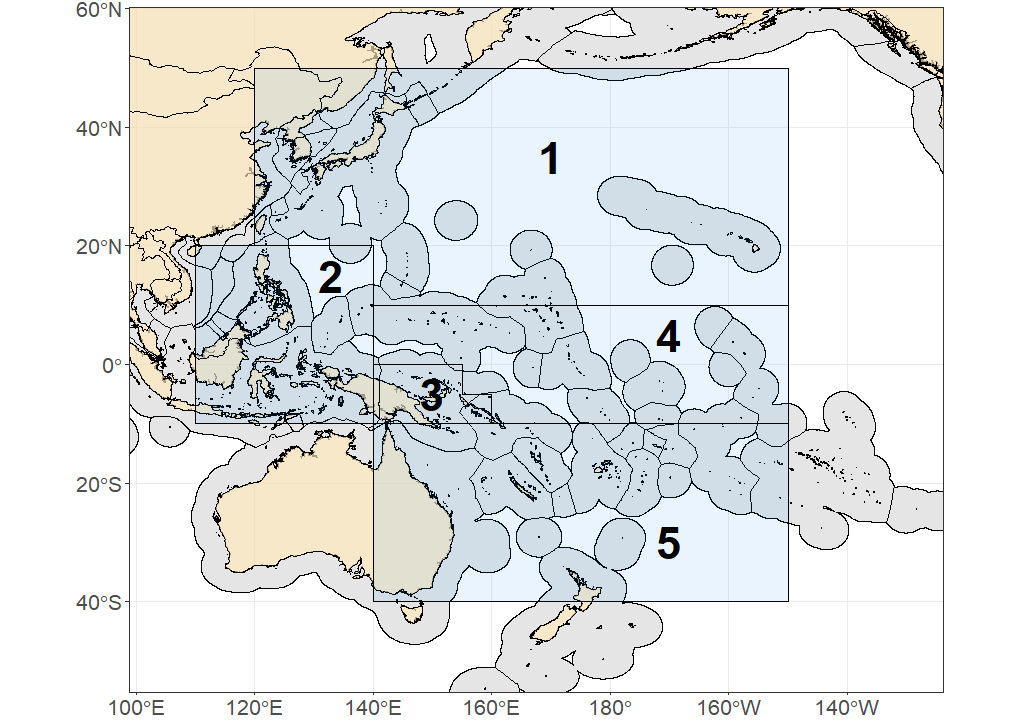
\includegraphics[width=0.7\textwidth]{map_5regions.png}\\[12mm]
  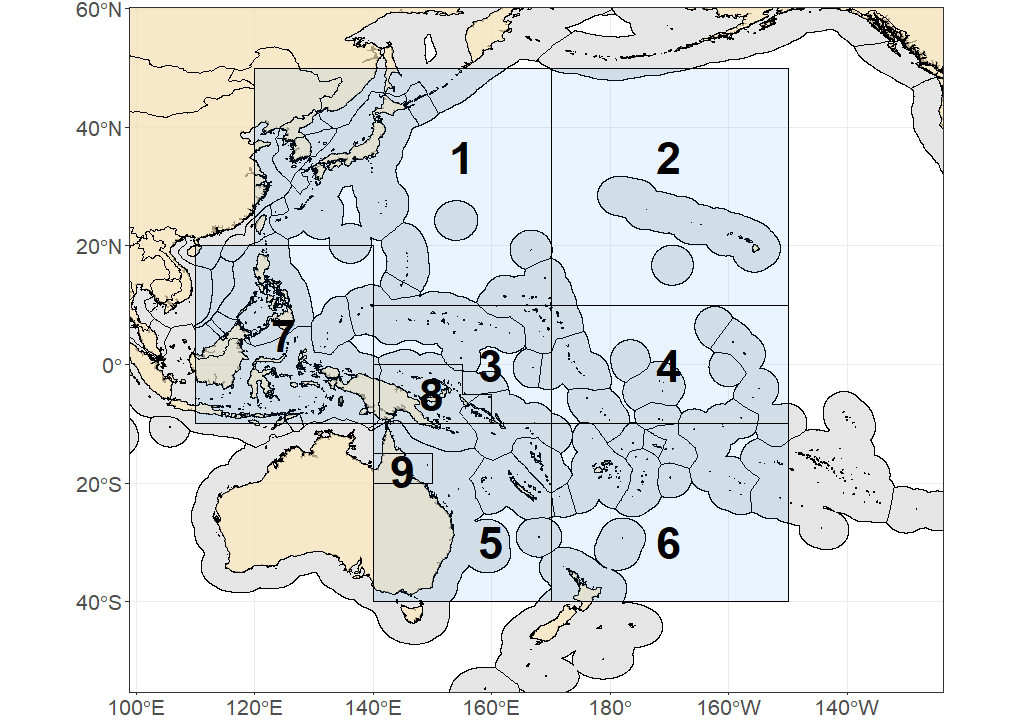
\includegraphics[width=0.7\textwidth]{map_9regions.png}\\[3mm]
  \caption{The geographical area covered by the stock assessment and the boundaries of the model regions for the 5 region structure that was used for 2023 WCPO yellowfin tuna assessment (top), and (bottom) the previous 9 region model structure that was used as the base structure for the stepwise model development.
    \label{fig:map_5regions_9regions}}
\end{figure}
\clearpage

\newpage
\begin{figure}[!ht]
  \centering
  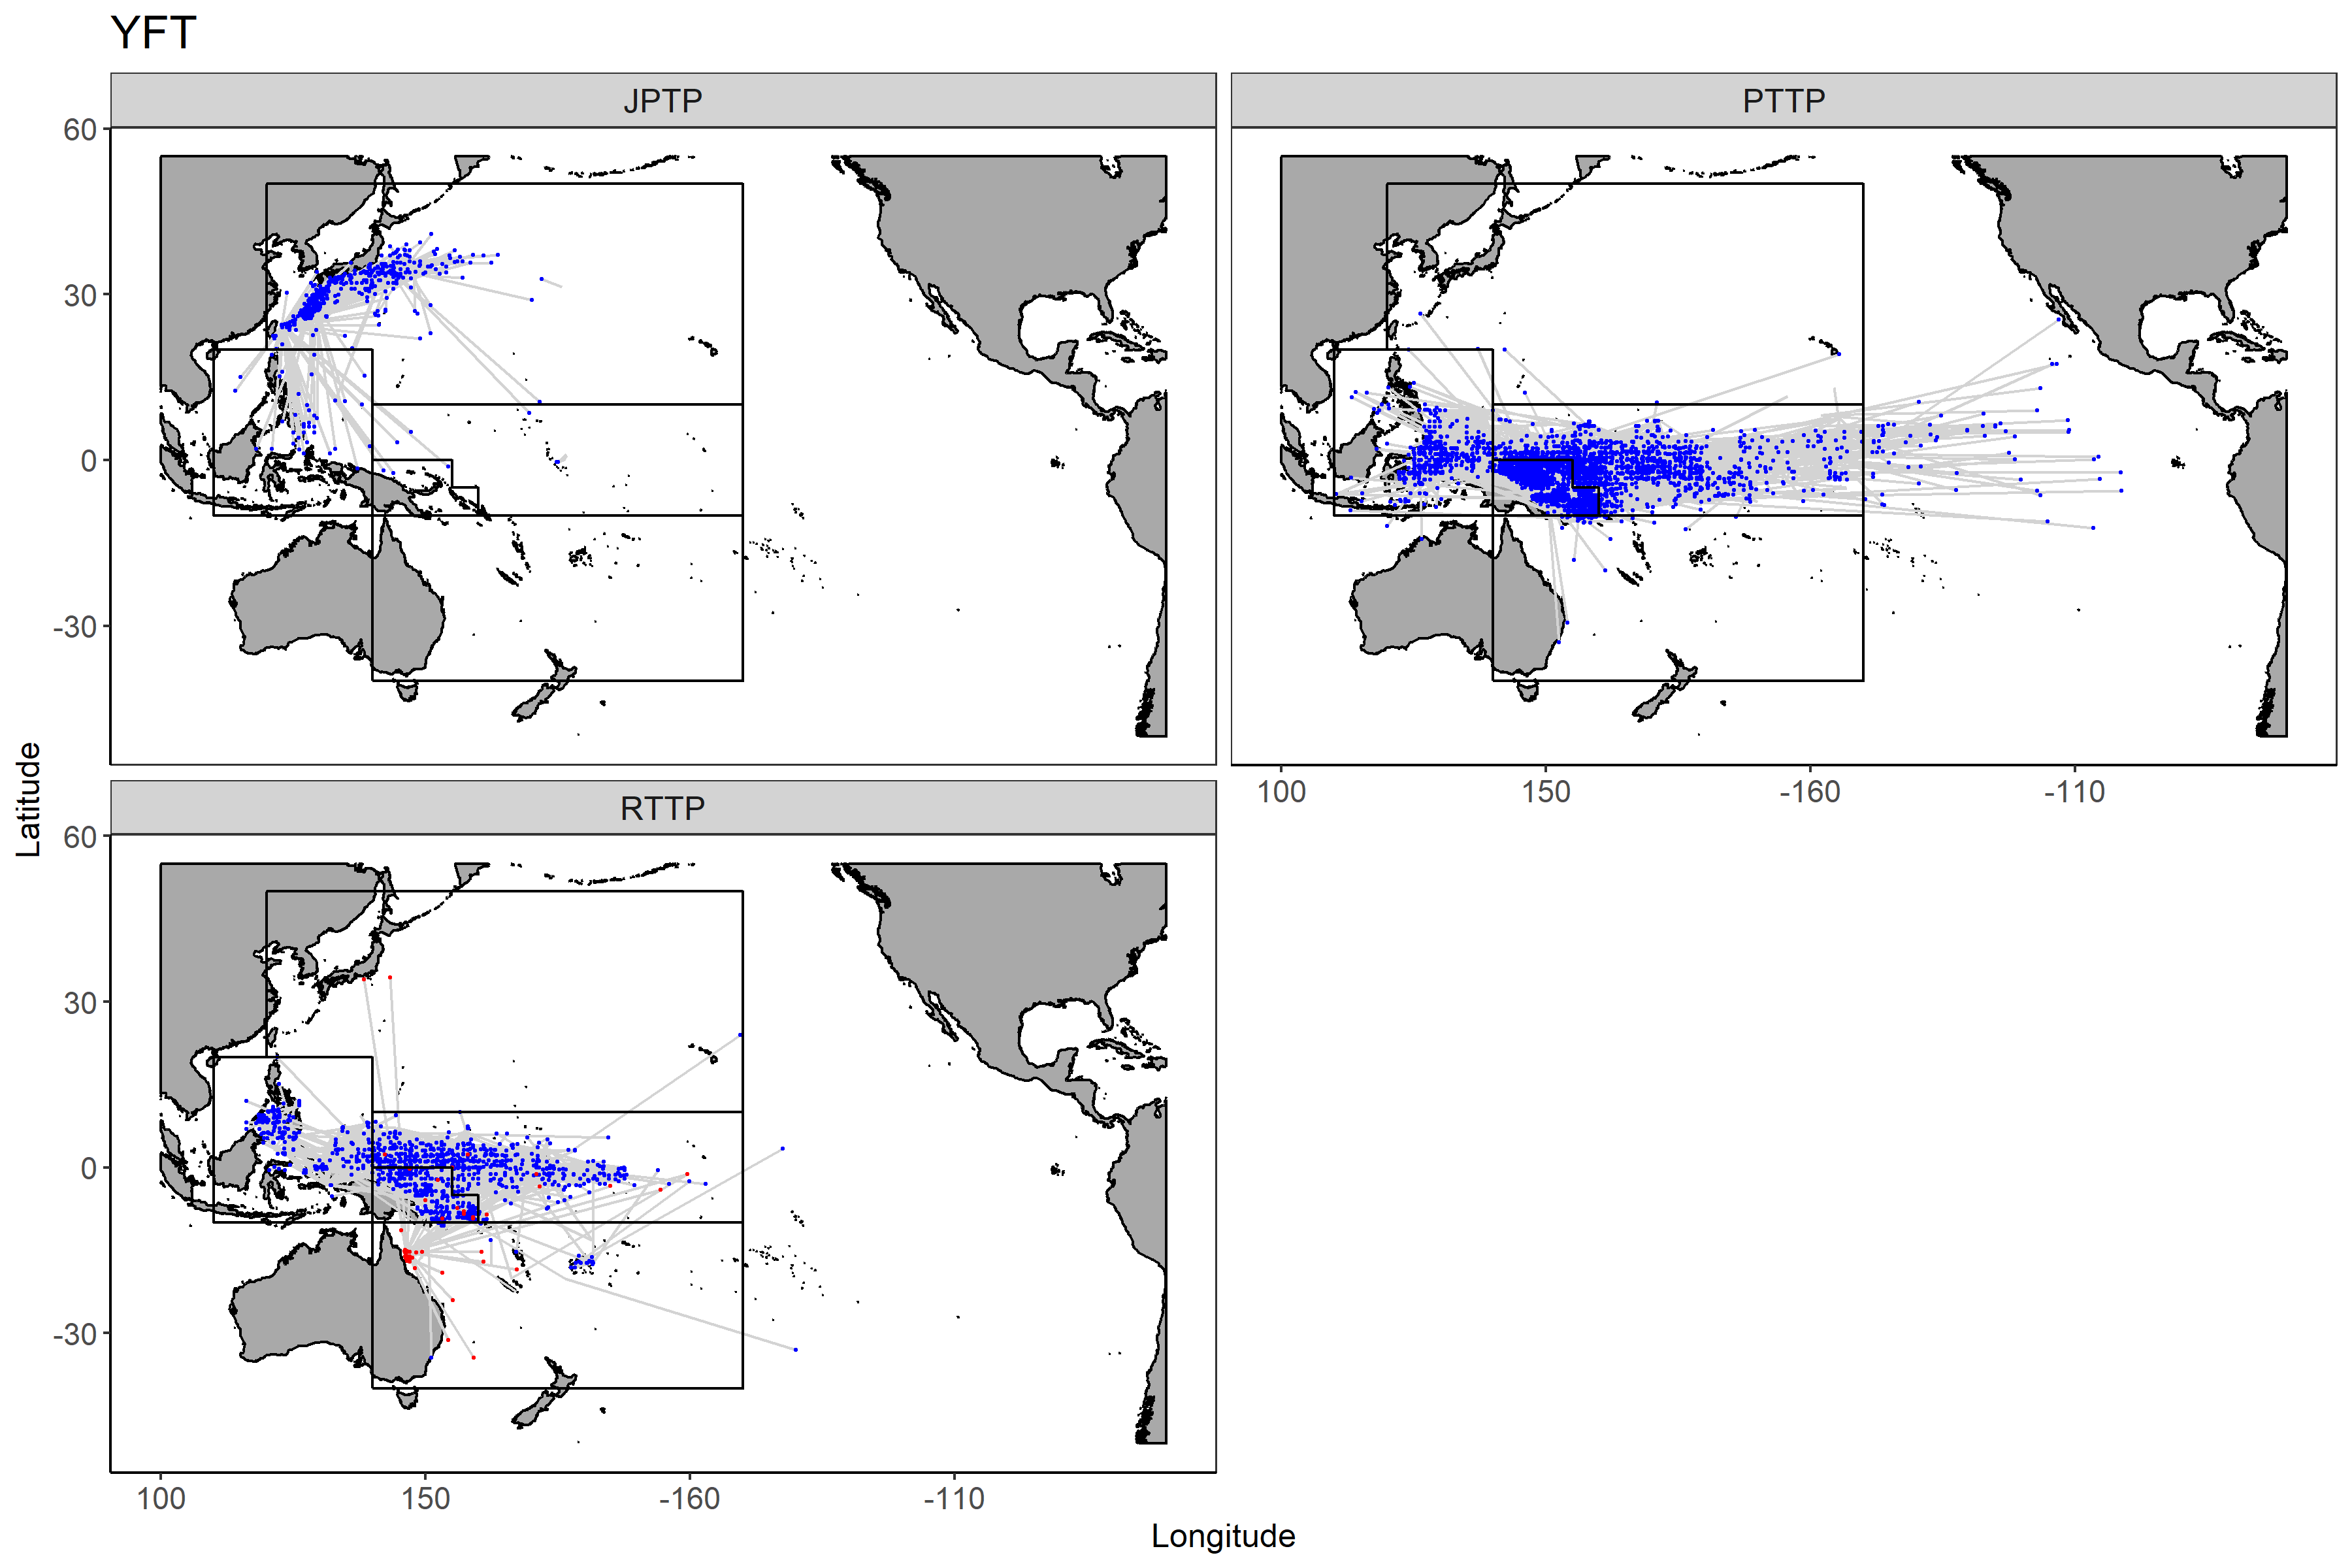
\includegraphics[width=1.0\textwidth]{tag_displacement_map.png}
  \caption{Map of tag recaptures. The panels show the distributions of release and recapture displacements for the different tagging programs: Pacific Tuna Tagging Program (PTTP), Regional Tuna Tagging Program (RTTP) and the Japanese Tagging Program (JPTP). Dots indicate recapture locations. Red dots in RTTP plot are the targeted Coral Sea tagging cruises. \label{fig:tag_displacement_map}}
\end{figure}
\clearpage

\newpage
\begin{figure}[!ht]
  \centering
  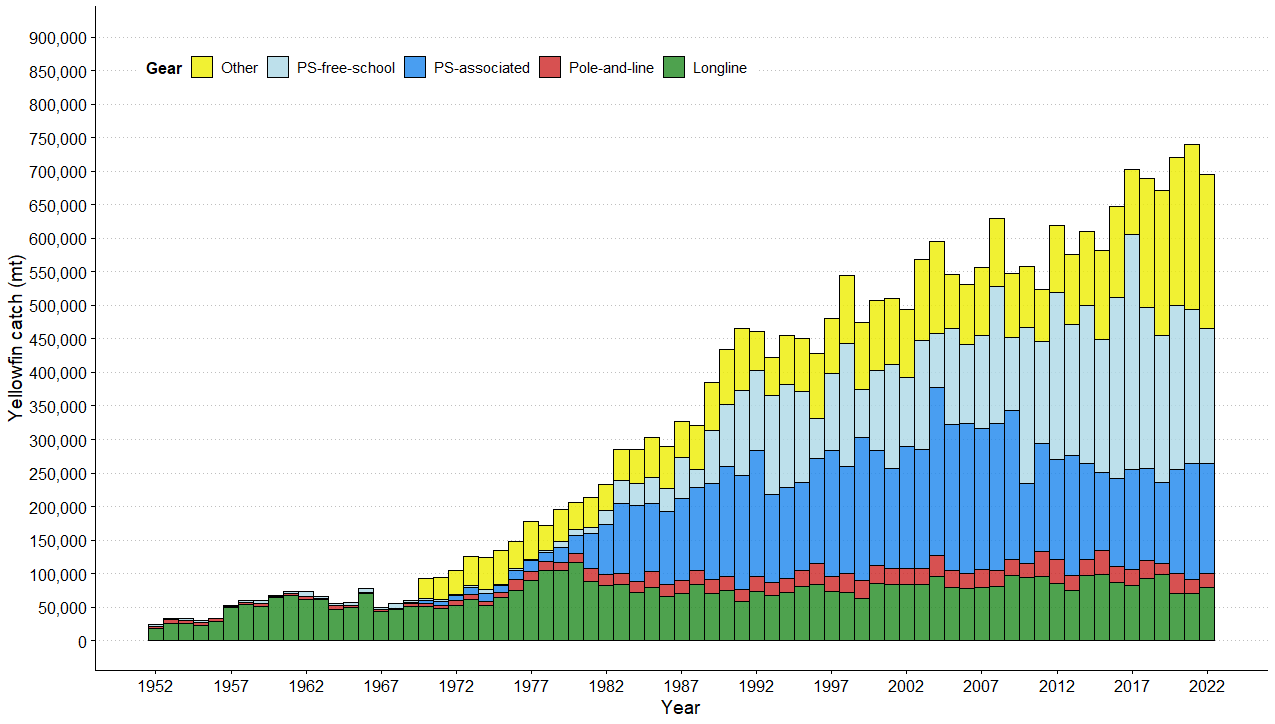
\includegraphics[width=1\textwidth]{catch_hist_full.png}
  \caption{Annual catches of yellowfin by gear type in the WCPO area covered by the assessment. \label{fig:catch_hist_full}}
\end{figure}
\clearpage

\newpage
\begin{figure}[!ht]
  \centering
  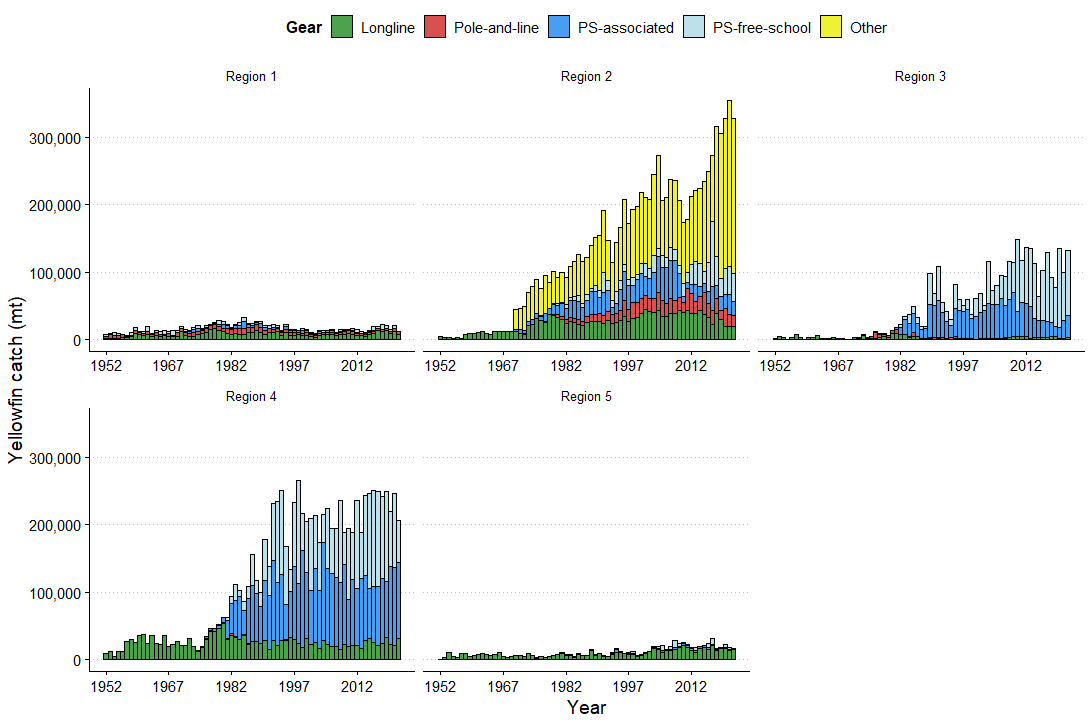
\includegraphics[width=1\textwidth]{catch_hist_regional.png}
  \caption{Annual catches of yellowfin by gear type for each of the five model regions. \label{fig:catch_hist_regional}}
\end{figure}
\clearpage

\newpage
\begin{figure}[!ht]
  \centering
  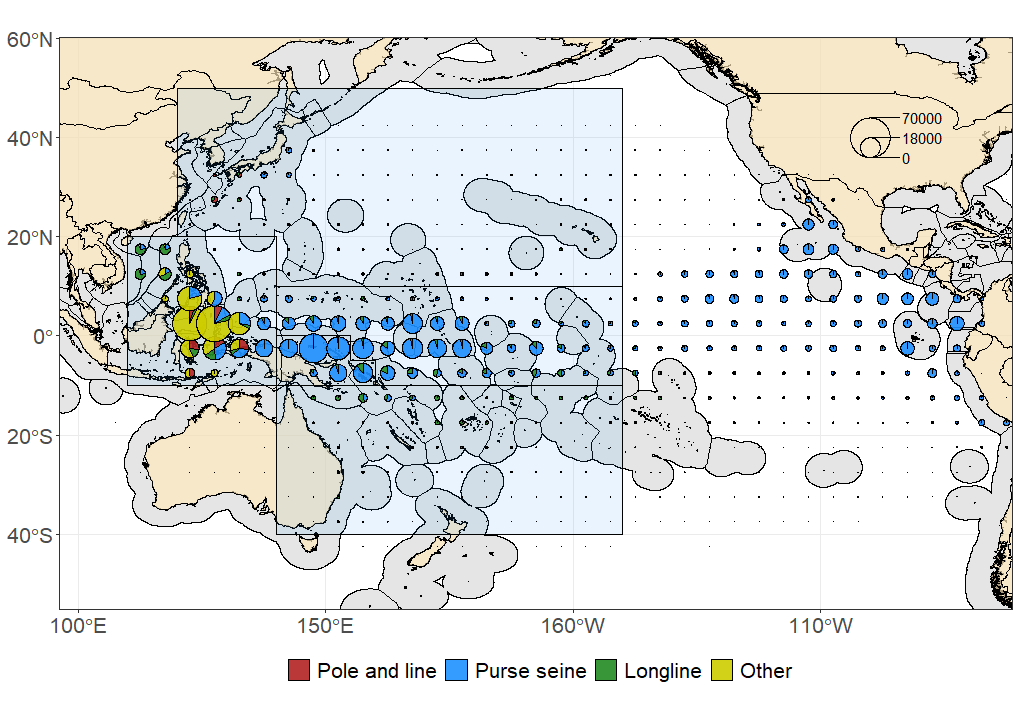
\includegraphics[width=\textwidth]{catch_map.png}
  \caption{Distribution and magnitude of yellowfin catches (mt) by gear type summed over the last 10 years (2012--2021) for 5 $\times$ 5 degree cells. \label{fig:catch_map}}
\end{figure}
\clearpage

\newpage
\begin{landscape}
  \begin{figure}[!ht]
    \centering
    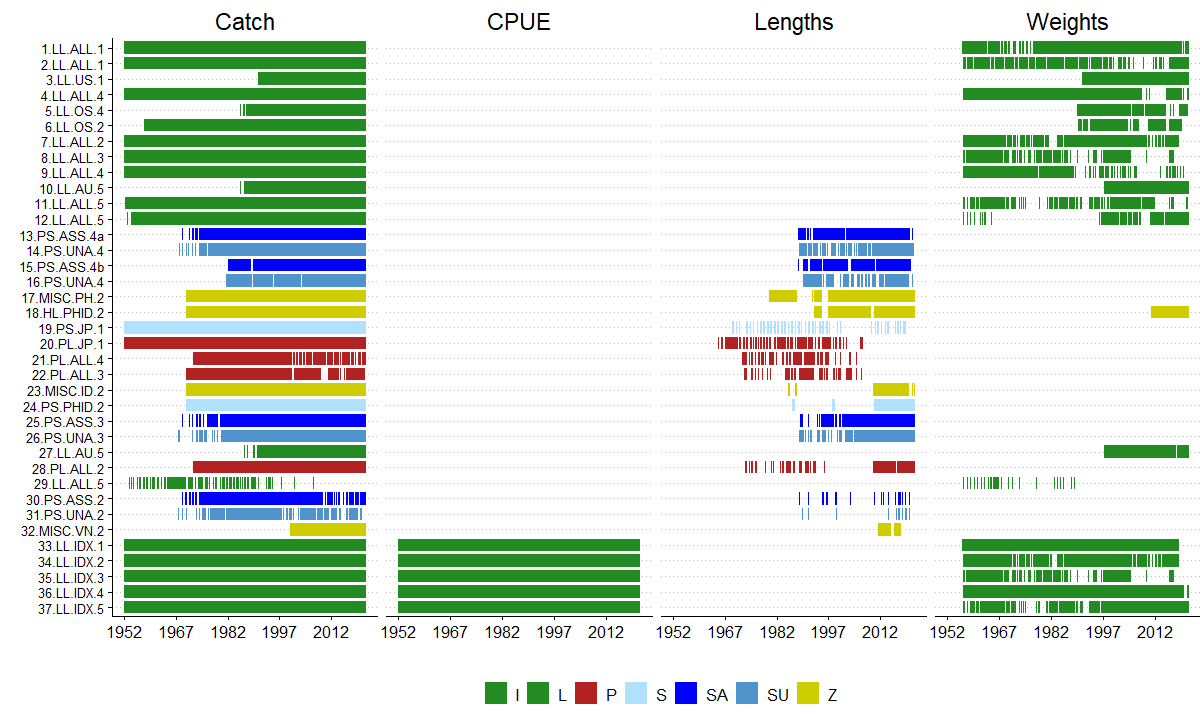
\includegraphics[width=1.3\textwidth]{data_coverage_tile.png}
    \caption{Summary of data coverage by fishery for the WCPO 2023 yellowfin assessment. I=index fisheries, L=longline, P=pole and line, S=purse seine (unspecified), SA=purse seine associated, SU=purse seine unassociated, Z=miscellaneous gears. \label{fig:data_coverage_tile}}
  \end{figure}
\end{landscape}
\clearpage

\newpage
\begin{landscape}
  \begin{figure}[H]
    \centering
    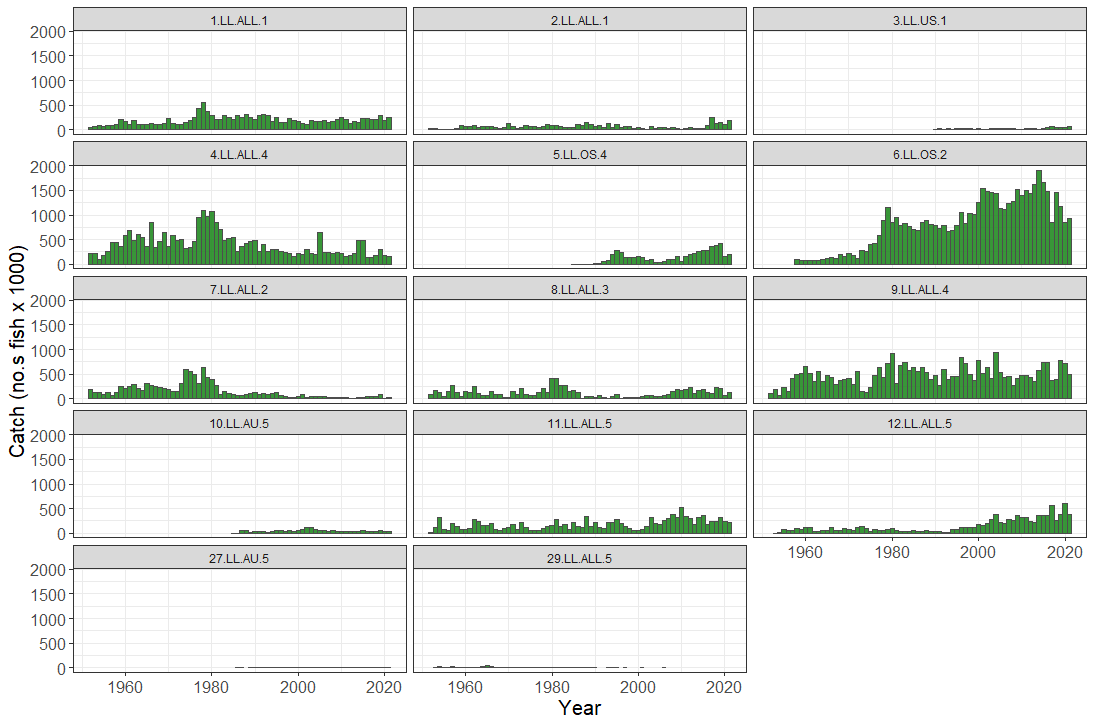
\includegraphics[width=1.2\textwidth]{catch_by_fishery_longline.png}
    \caption{Time series of annual catches (numbers of fish) by fishery: longline. \label{fig:catch_by_fishery_longline}}
  \end{figure}

  \begin{figure}[H]
    \centering
    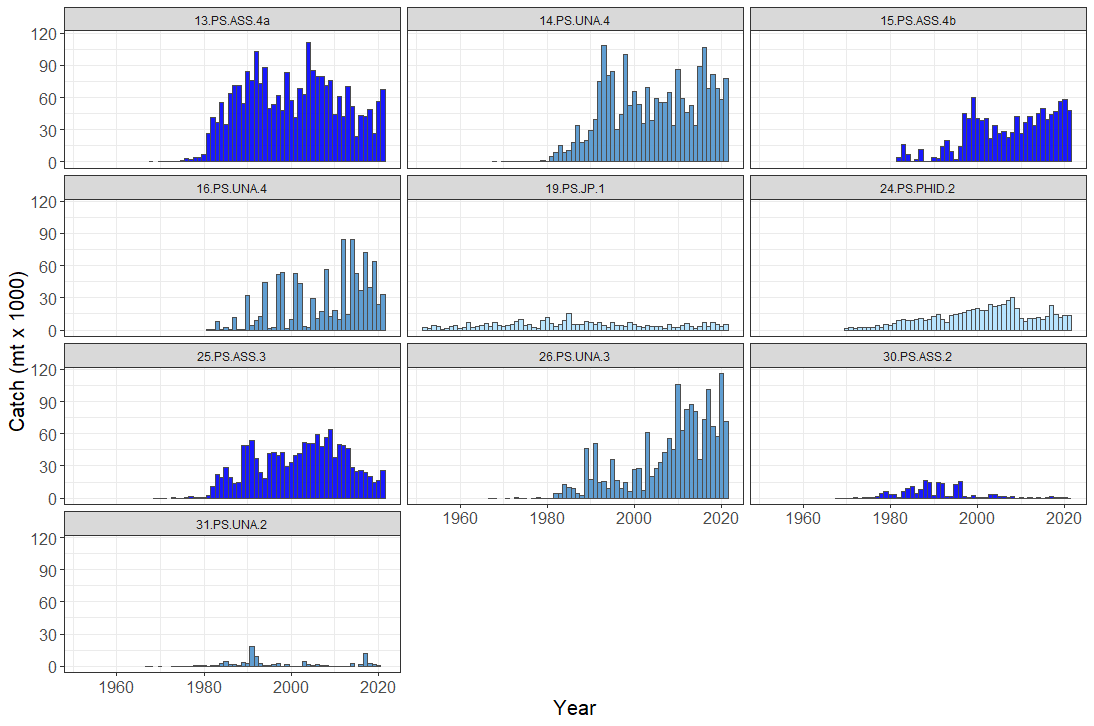
\includegraphics[width=1.2\textwidth]{catch_by_fishery_ps.png}
    \caption{Time series of annual catches (mt) by fishery: purse seine. \label{fig:catch_by_fishery_ps}}
  \end{figure}

  \begin{figure}[H]
    \centering
    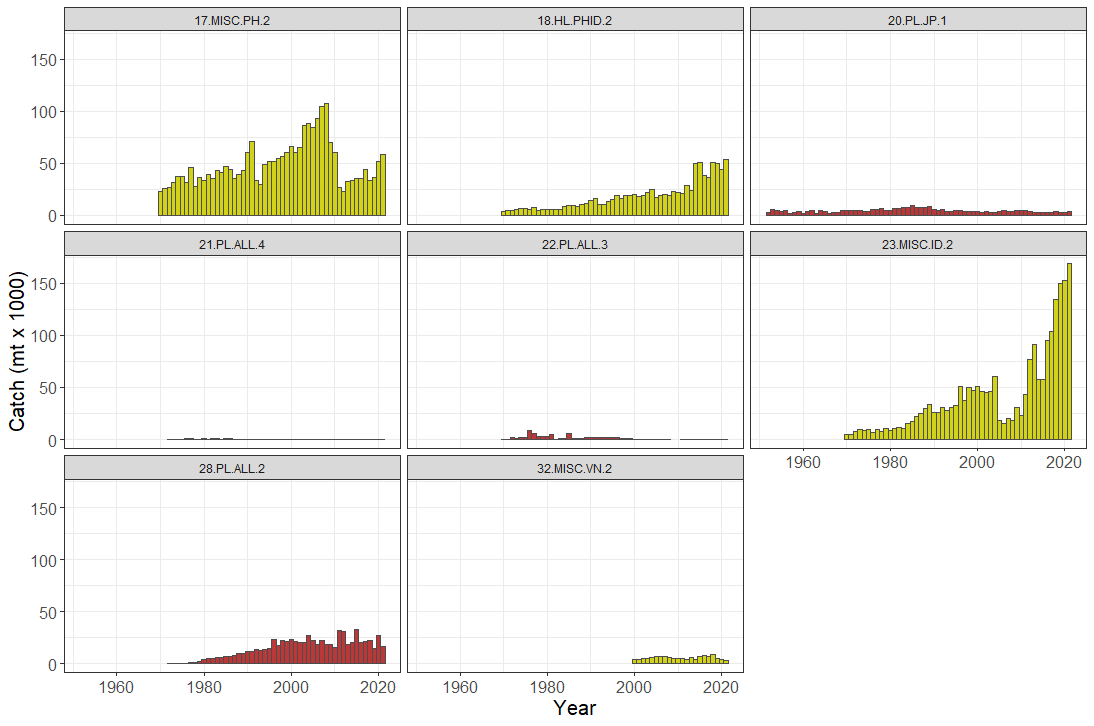
\includegraphics[width=1.2\textwidth]{catch_by_fishery_other.png}
    \caption{Time series of annual catches (mt) by fishery: other. \label{fig:catch_by_fishery_other}}
  \end{figure}
\end{landscape}
\clearpage

\newpage
\begin{landscape}
  \begin{figure}[!ht]
    \centering
    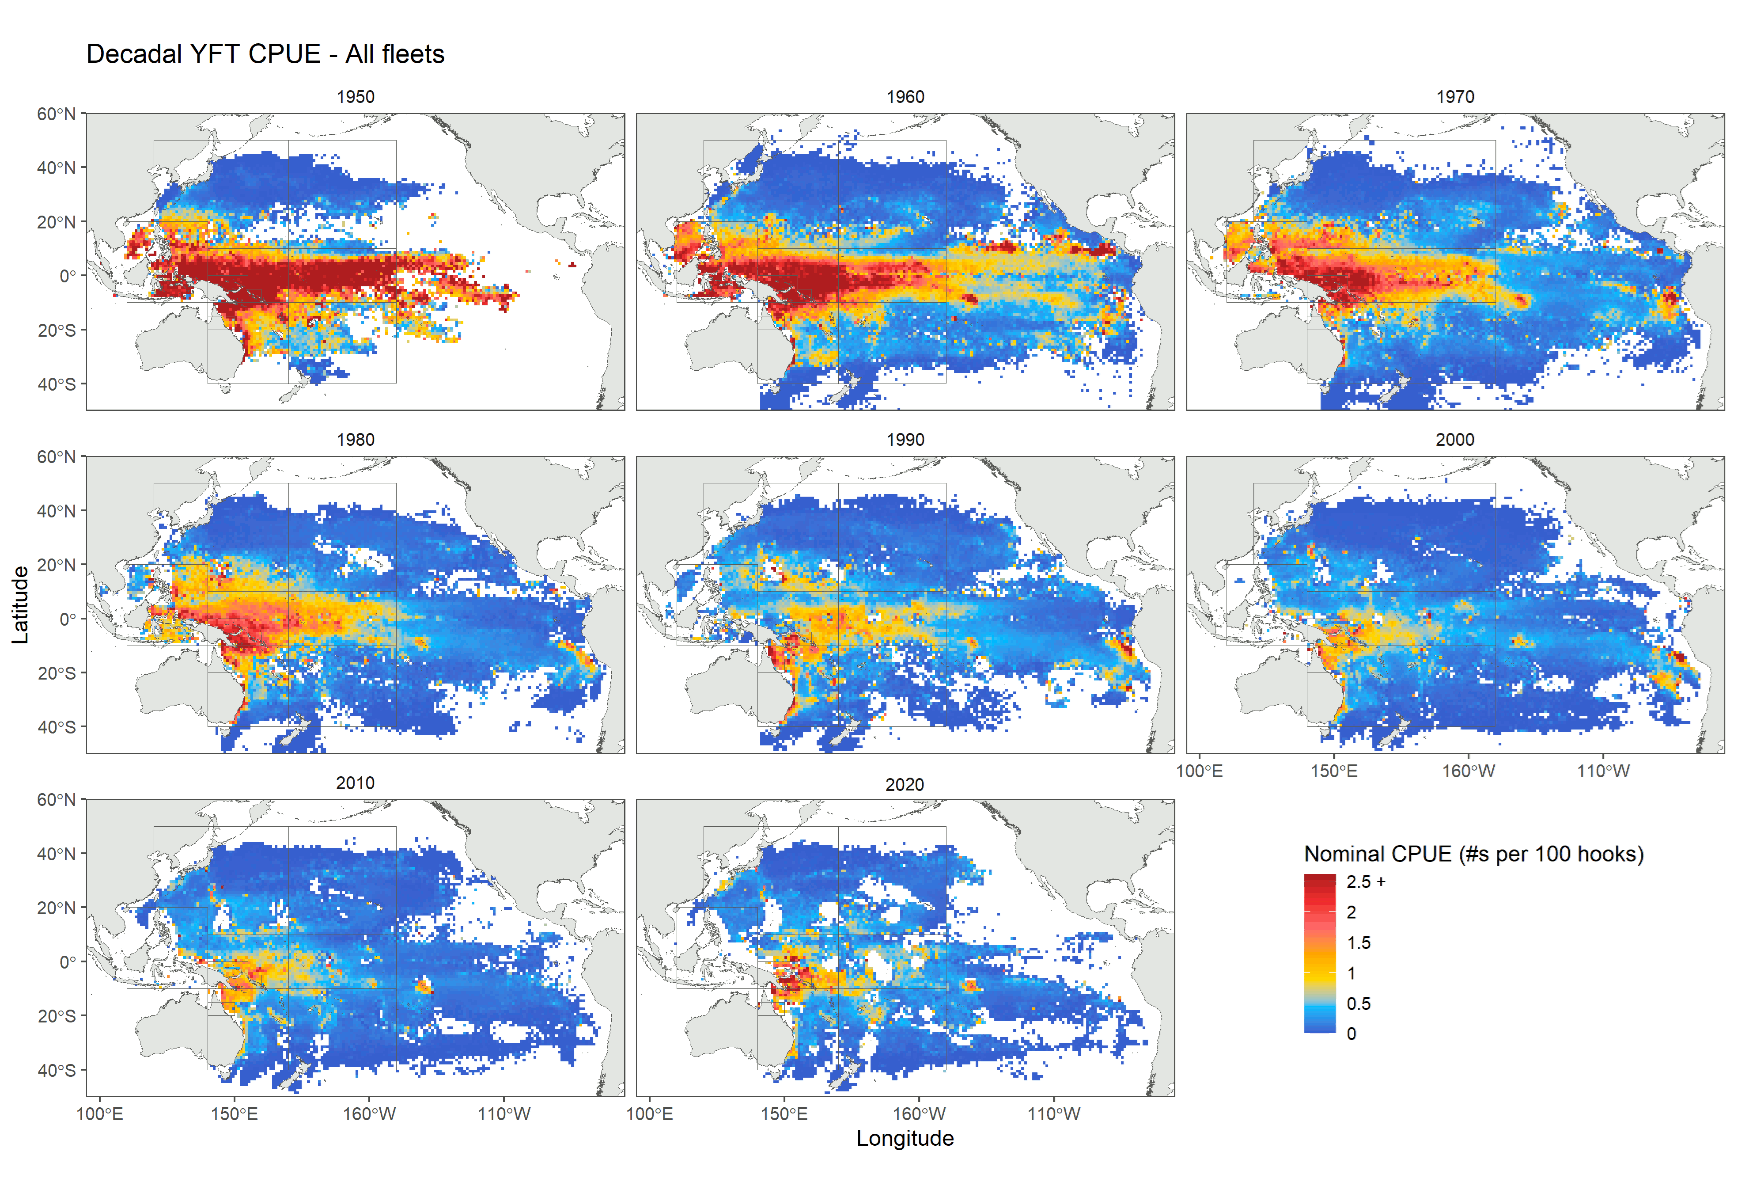
\includegraphics[width=1.3\textwidth]{cpue_nom_maps.png}
    \caption{Spatial distribution of nominal longline CPUE (all fleets) for yellowfin in the Pacific. \label{fig:cpue_nom_maps}}
  \end{figure}
\end{landscape}
\clearpage

\newpage
\begin{figure}[!ht]
  \centering
  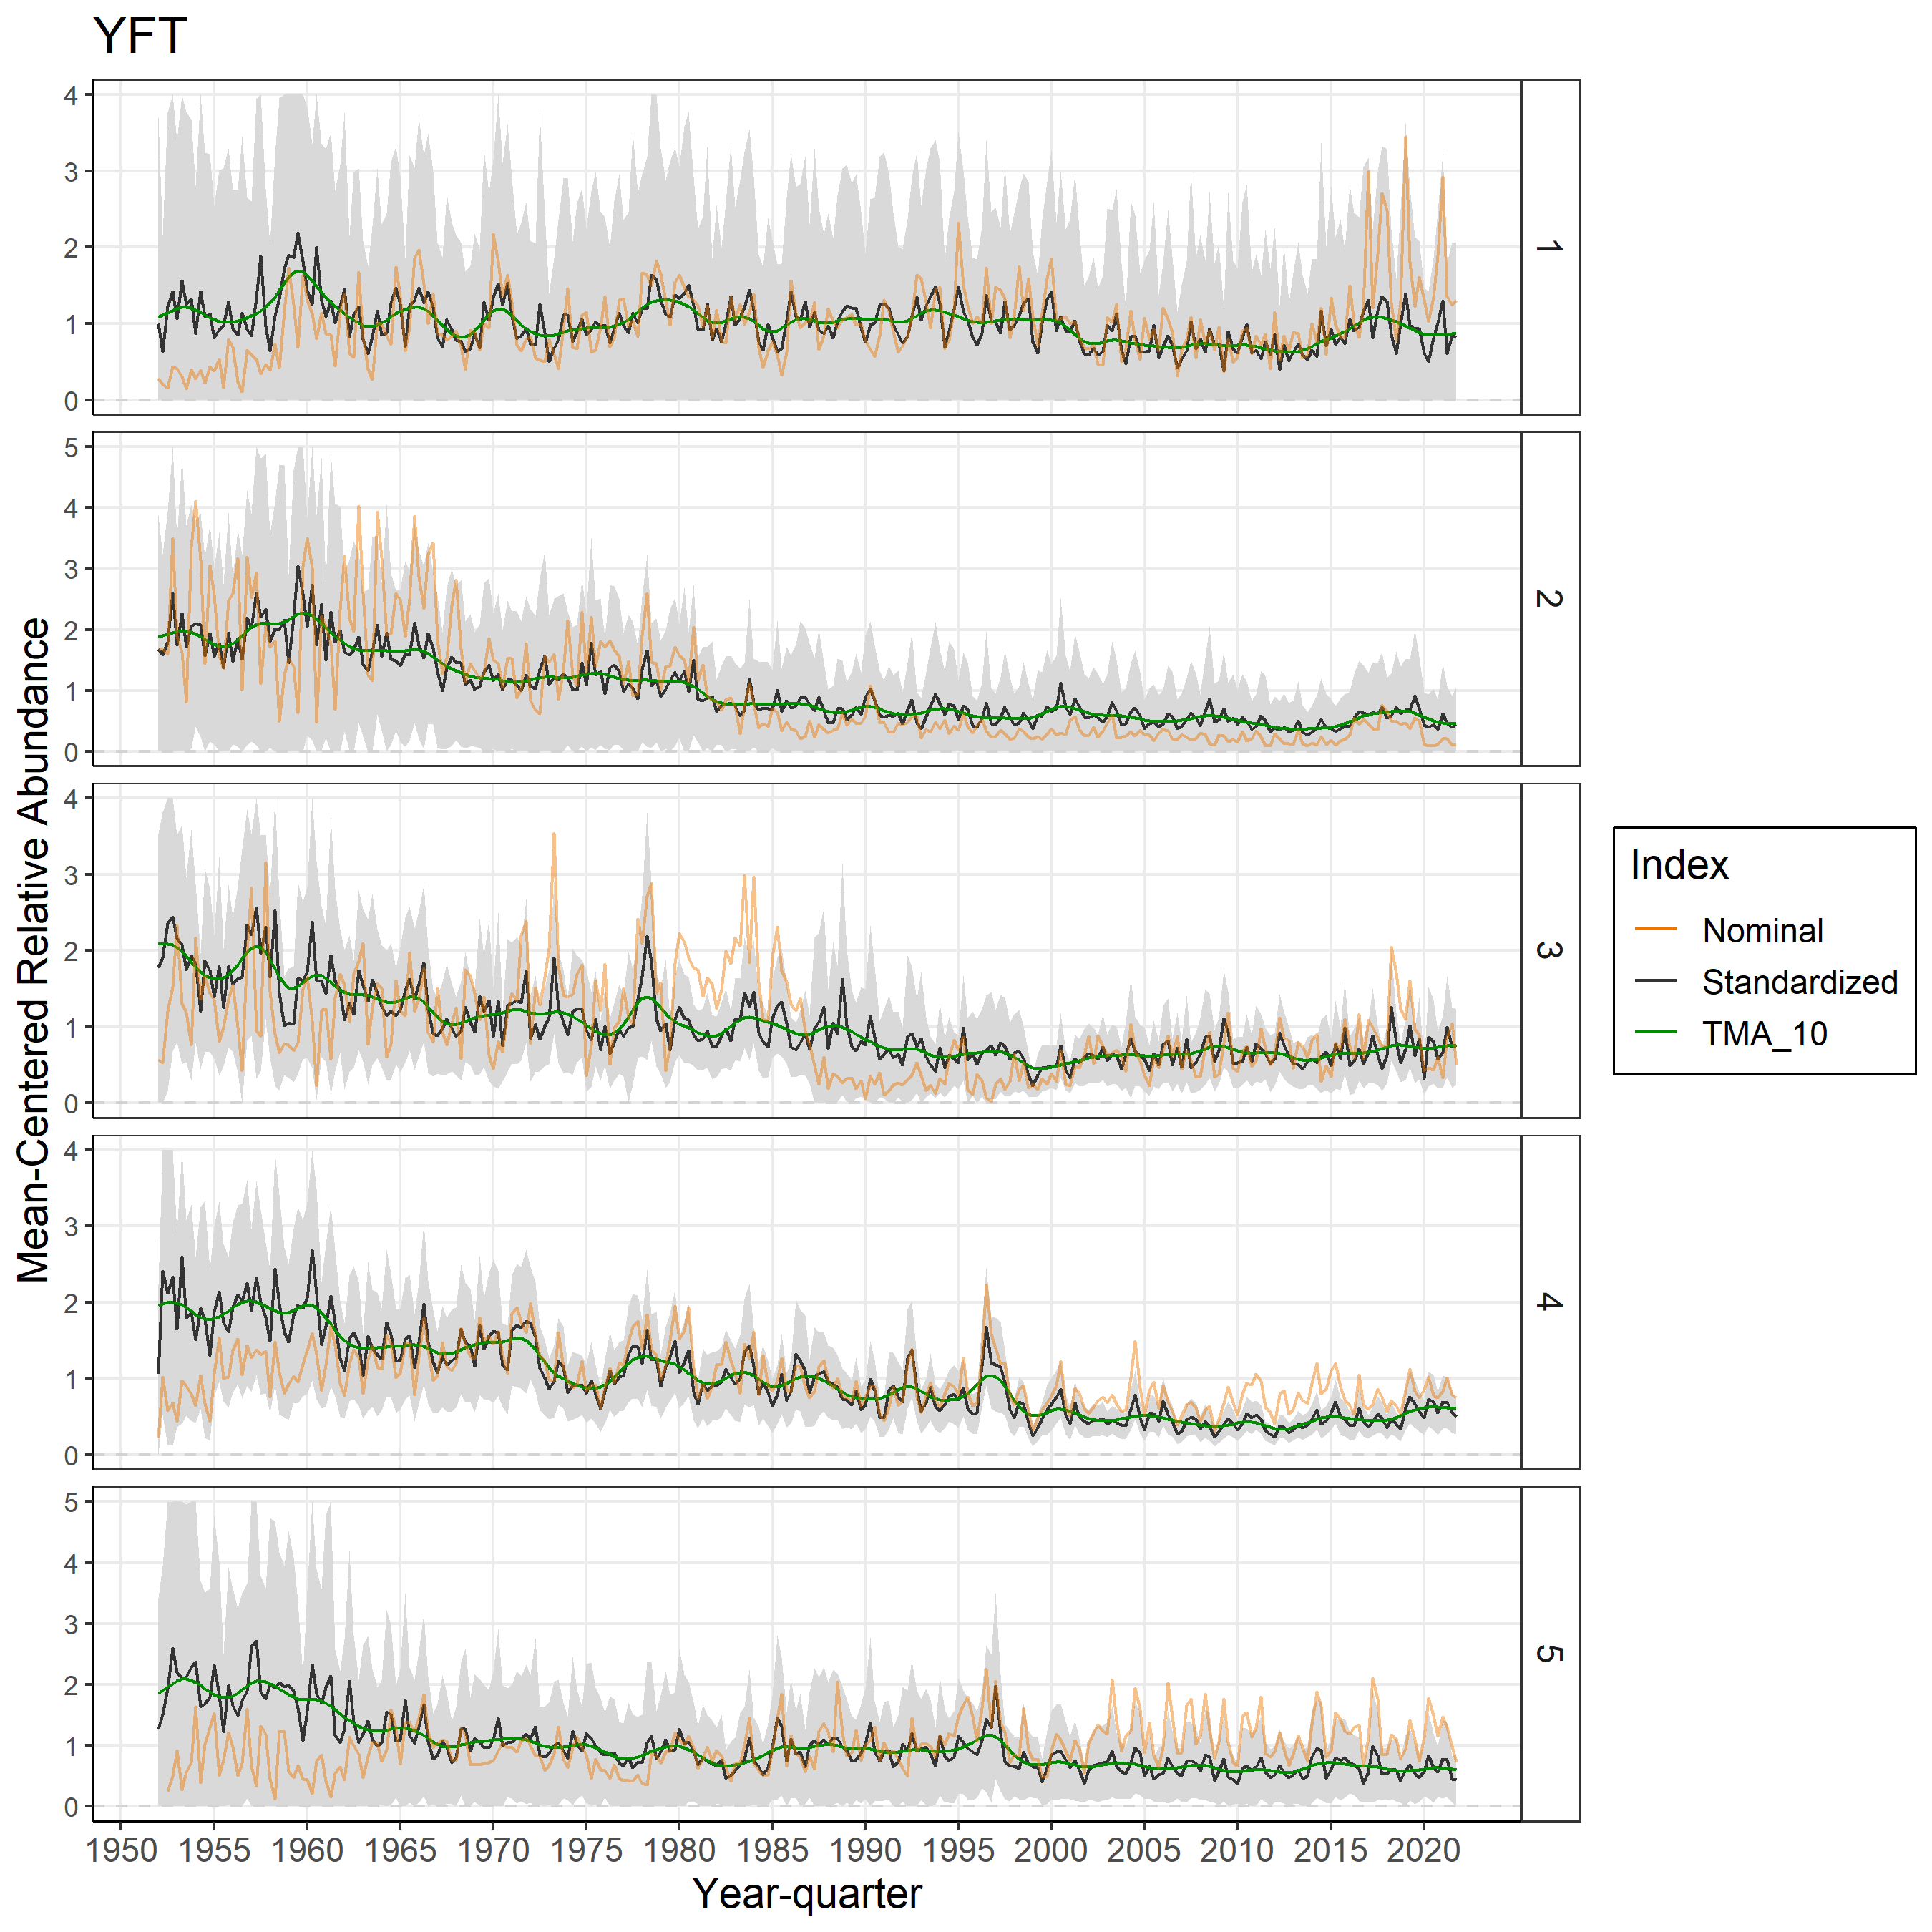
\includegraphics[width=1.08\textwidth]{cpue_nom_std_portrait.png}
  \caption{Standardised (black line) and nominal (orange) CPUE for the longline index fisheries in each model. Gray band is 95\% CI. Triangular moving average smoothing function applied to demonstrate overall trend (green line; smoothing window = 10). 	\label{fig:cpue_nom_std_1_5}}
\end{figure}
\clearpage
\newpage

\newpage
\begin{landscape}
  \begin{figure}[!ht]
    \centering
    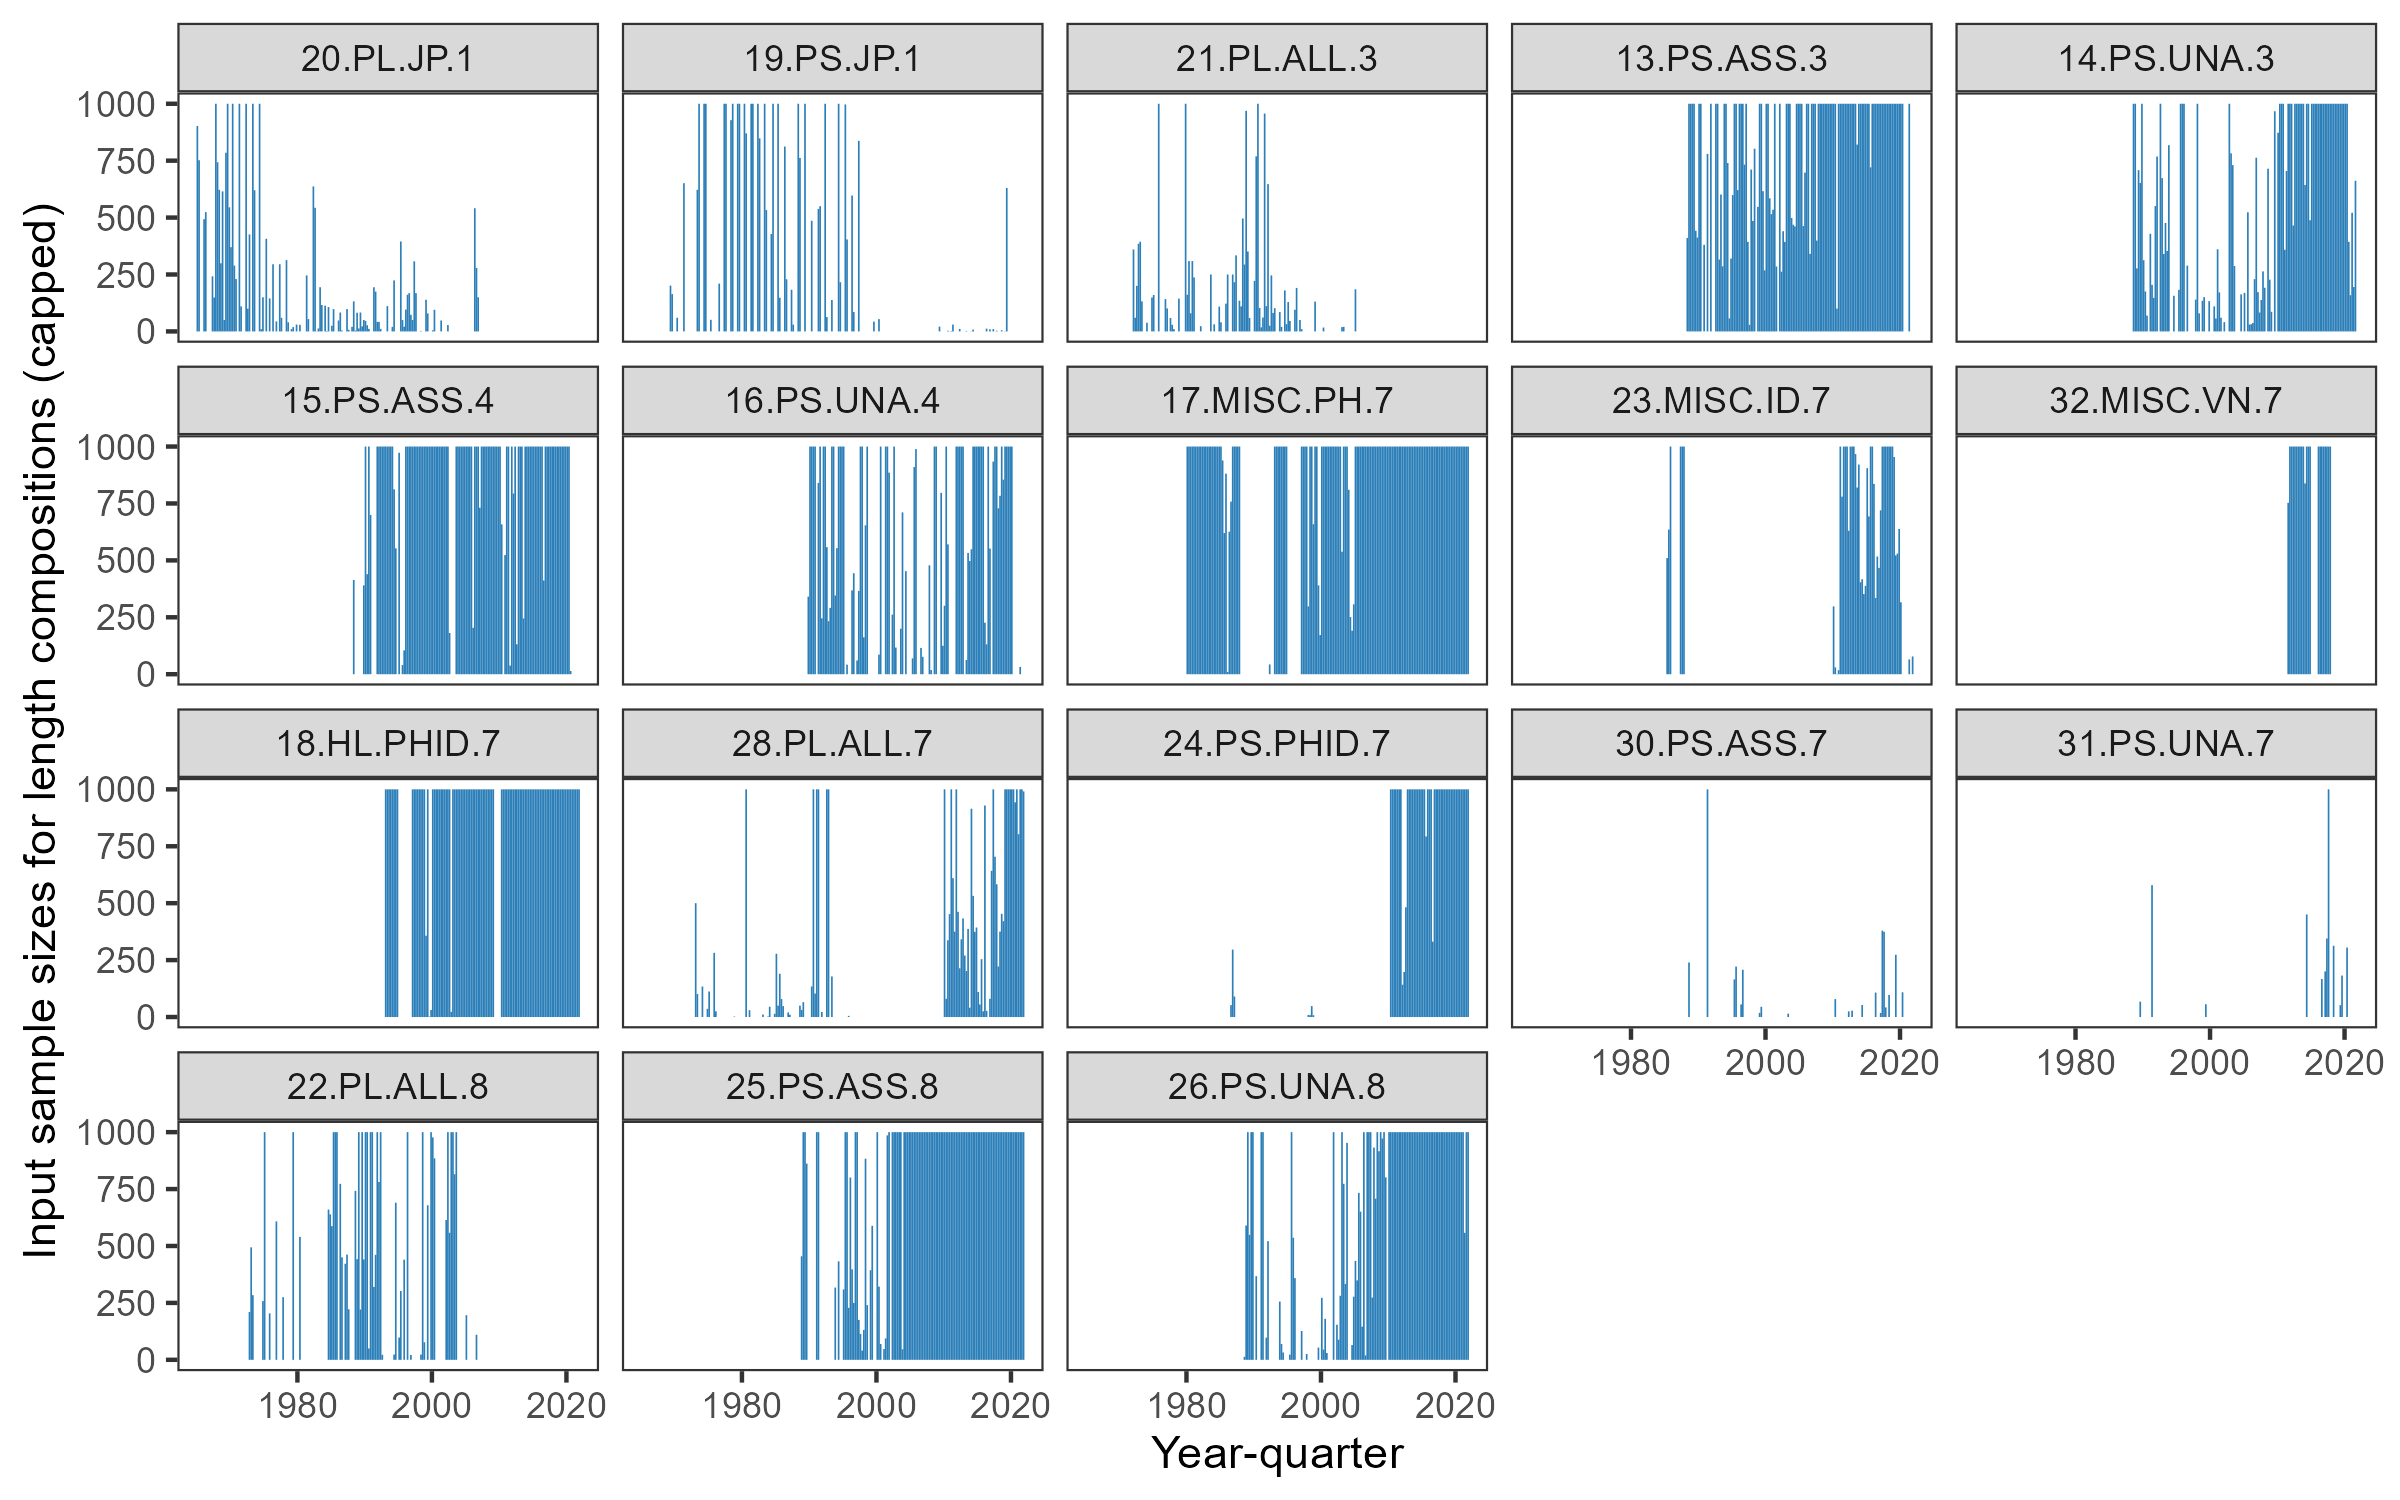
\includegraphics[width=1.2\textwidth]{length_comp_sampl_sum.png}
    \caption{Plots of samples sizes (capped at 1,000) for length composition for each fishery in the model across the model time period. \label{fig:length_comp_sampl_sum}}
  \end{figure}
\end{landscape}
\clearpage

\newpage
\begin{landscape}
  \begin{figure}[!ht]
    \centering
    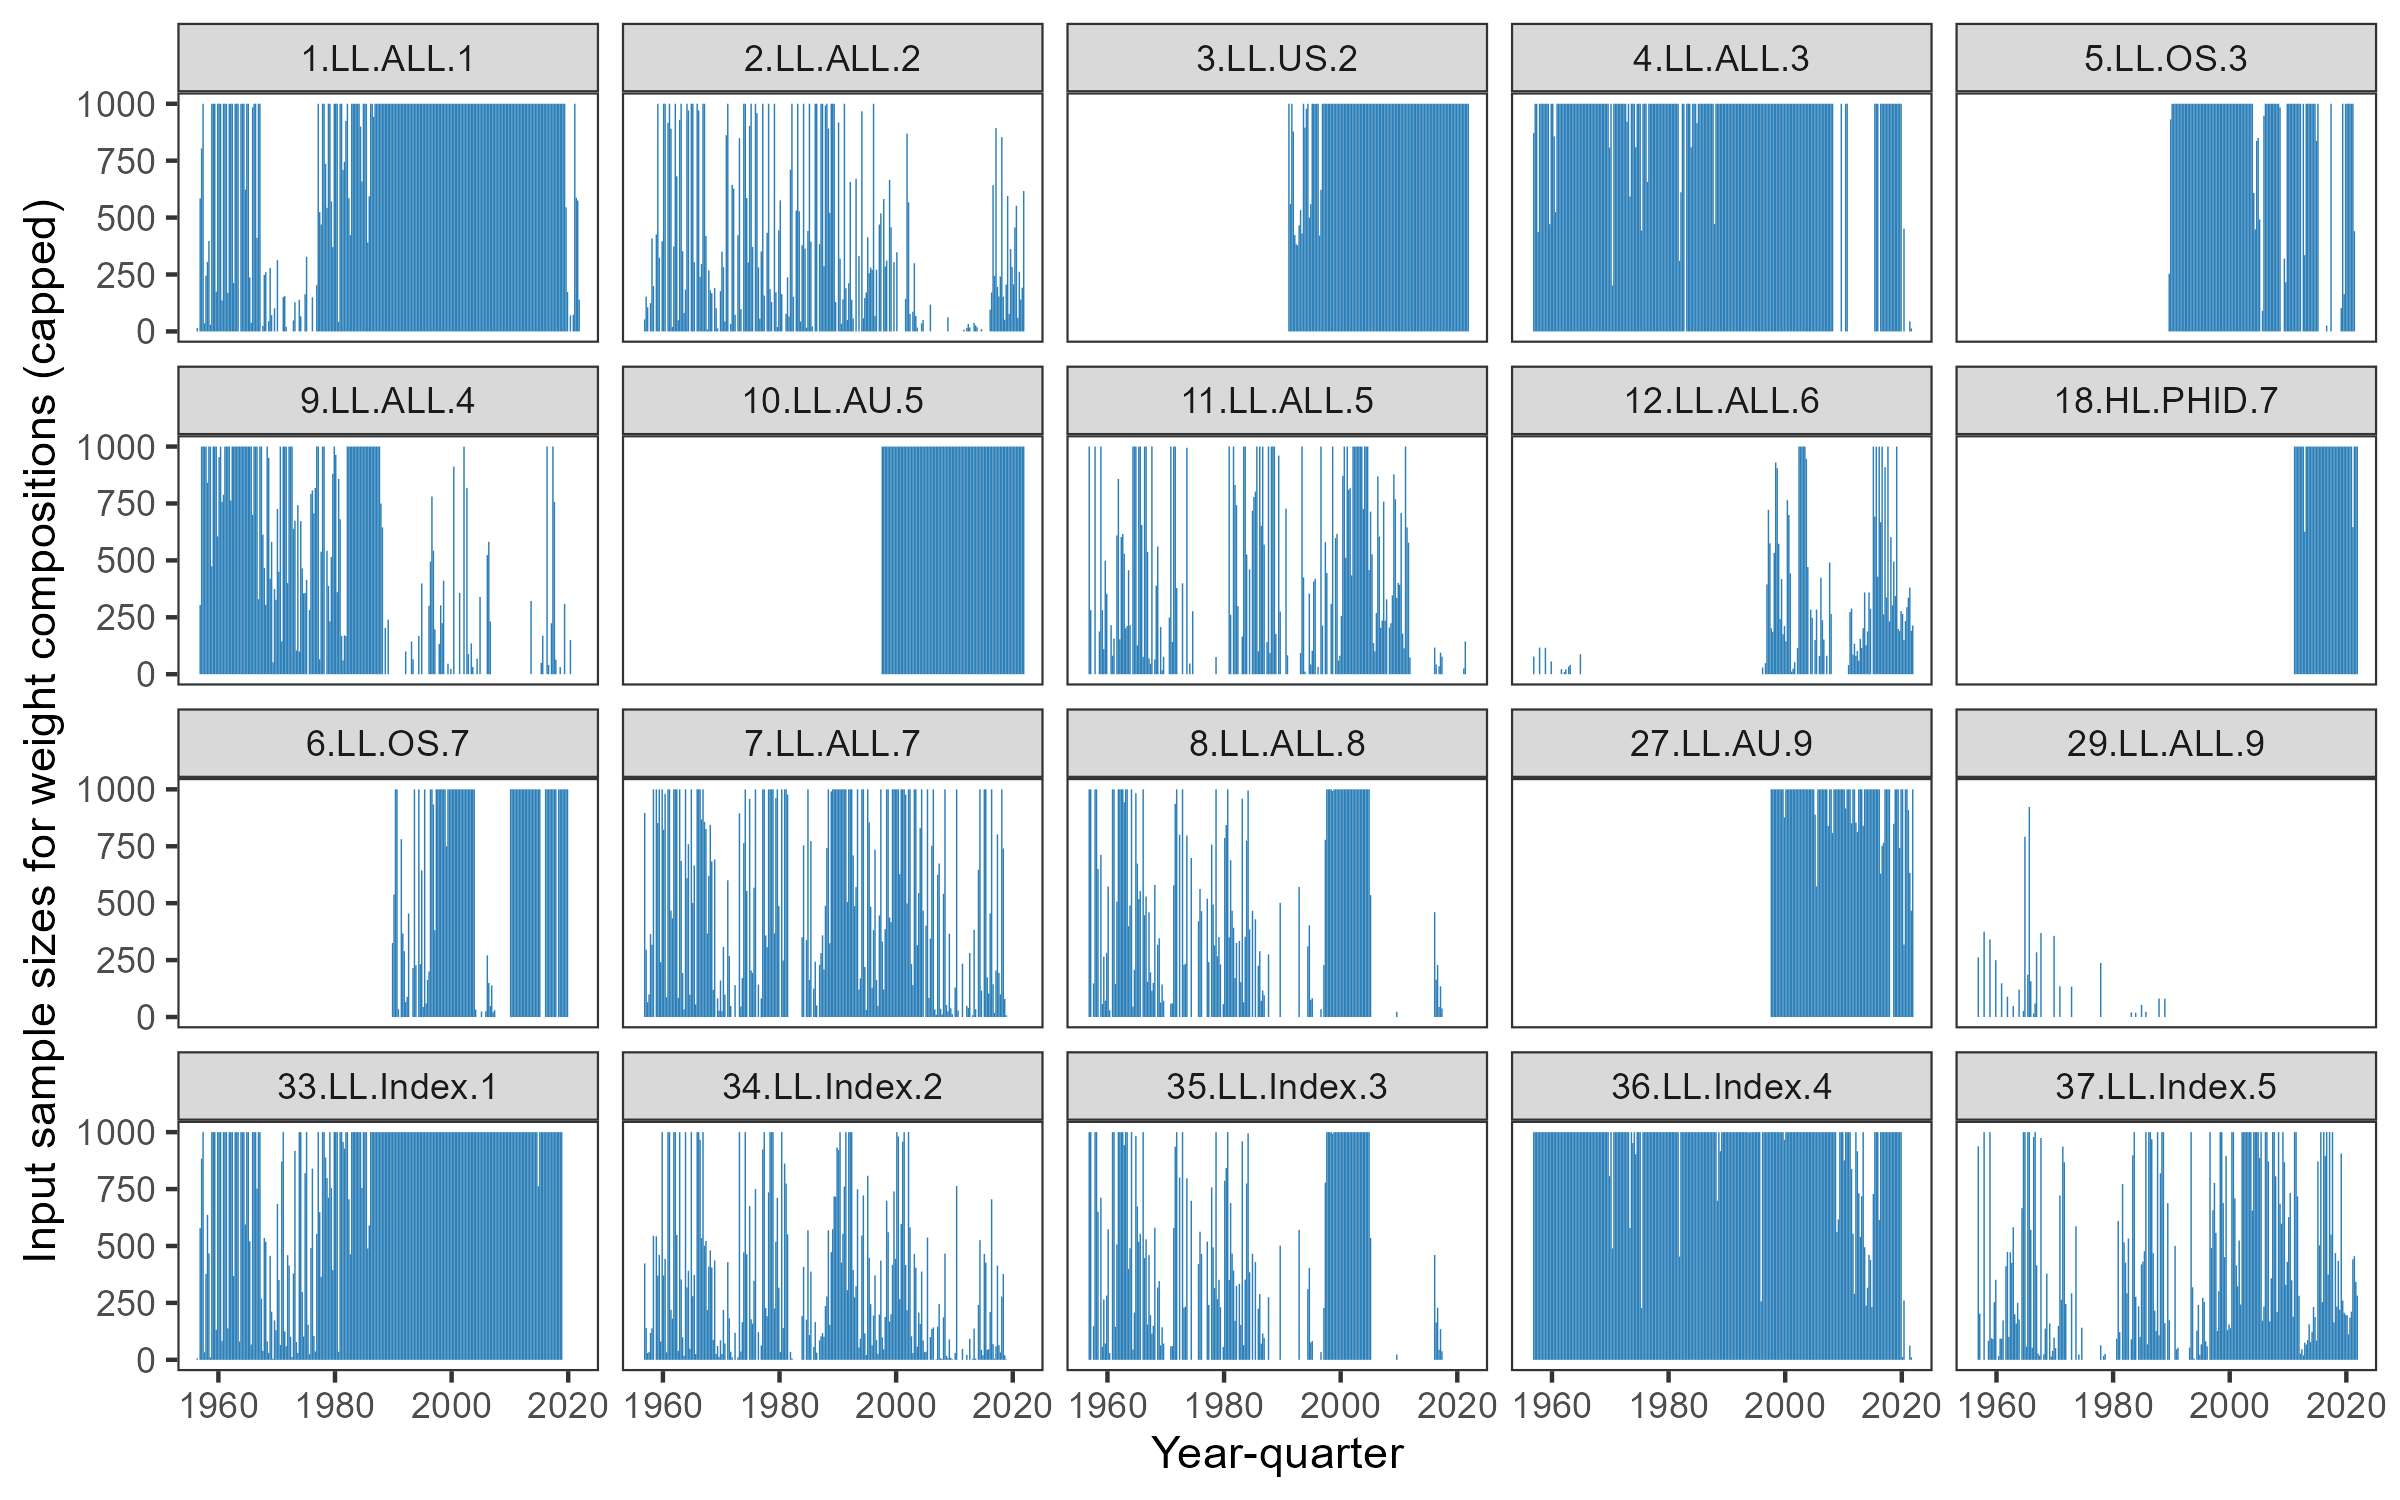
\includegraphics[width=1.2\textwidth]{weight_comp_sampl_sum.png}
    \caption{Plots of samples sizes (capped at 1,000) for weight composition for each fishery in the model across the model time period. \label{fig:size_comp_sampl_sum}}
  \end{figure}
\end{landscape}
\clearpage

\newpage
\begin{landscape}
  \begin{figure}[!ht]
    \centering
    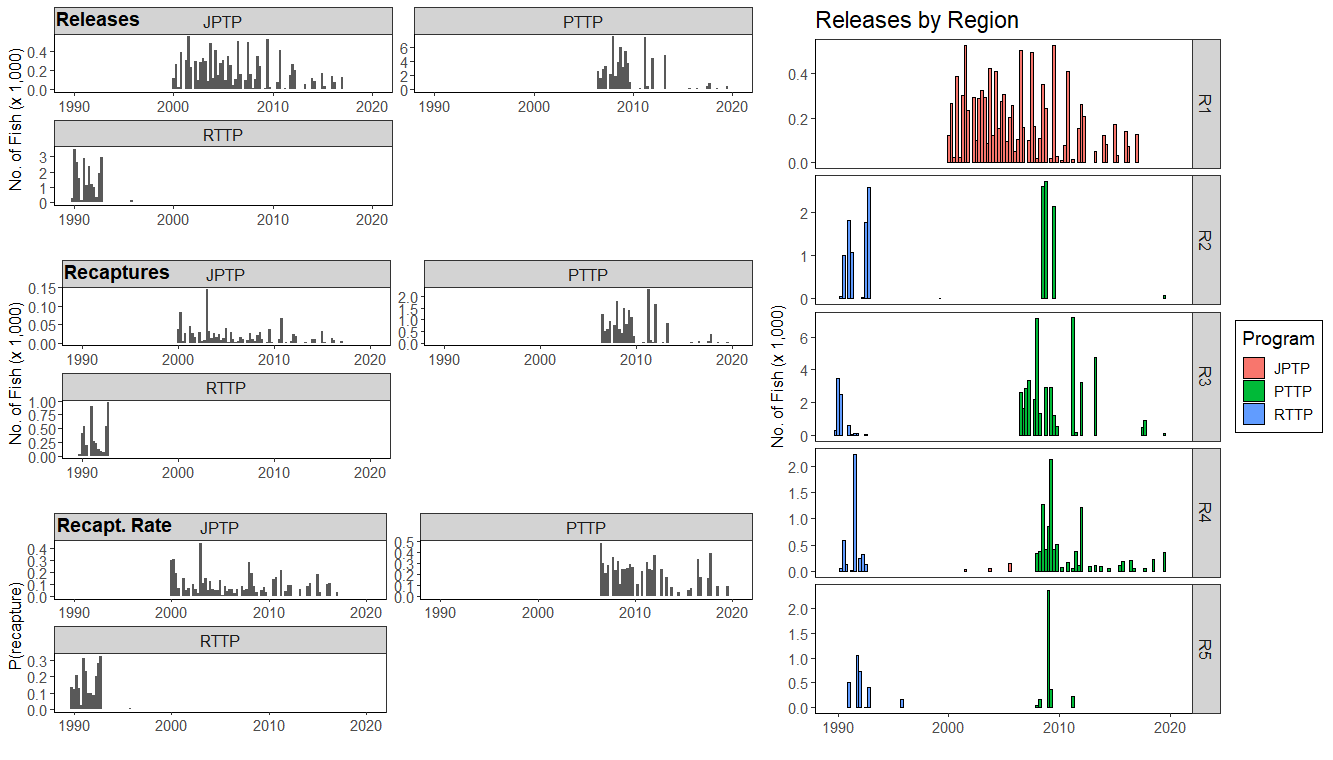
\includegraphics[width=1.35\textwidth]{tag_release_recapt.png}
    \caption{Summary plots of the number of releases, recaptures, and recapture rate of tags, by tagging program and region. \label{fig:tag_release_recapt}}
  \end{figure}
\end{landscape}
\clearpage

\newpage
\begin{figure}[!ht]
  \centering
  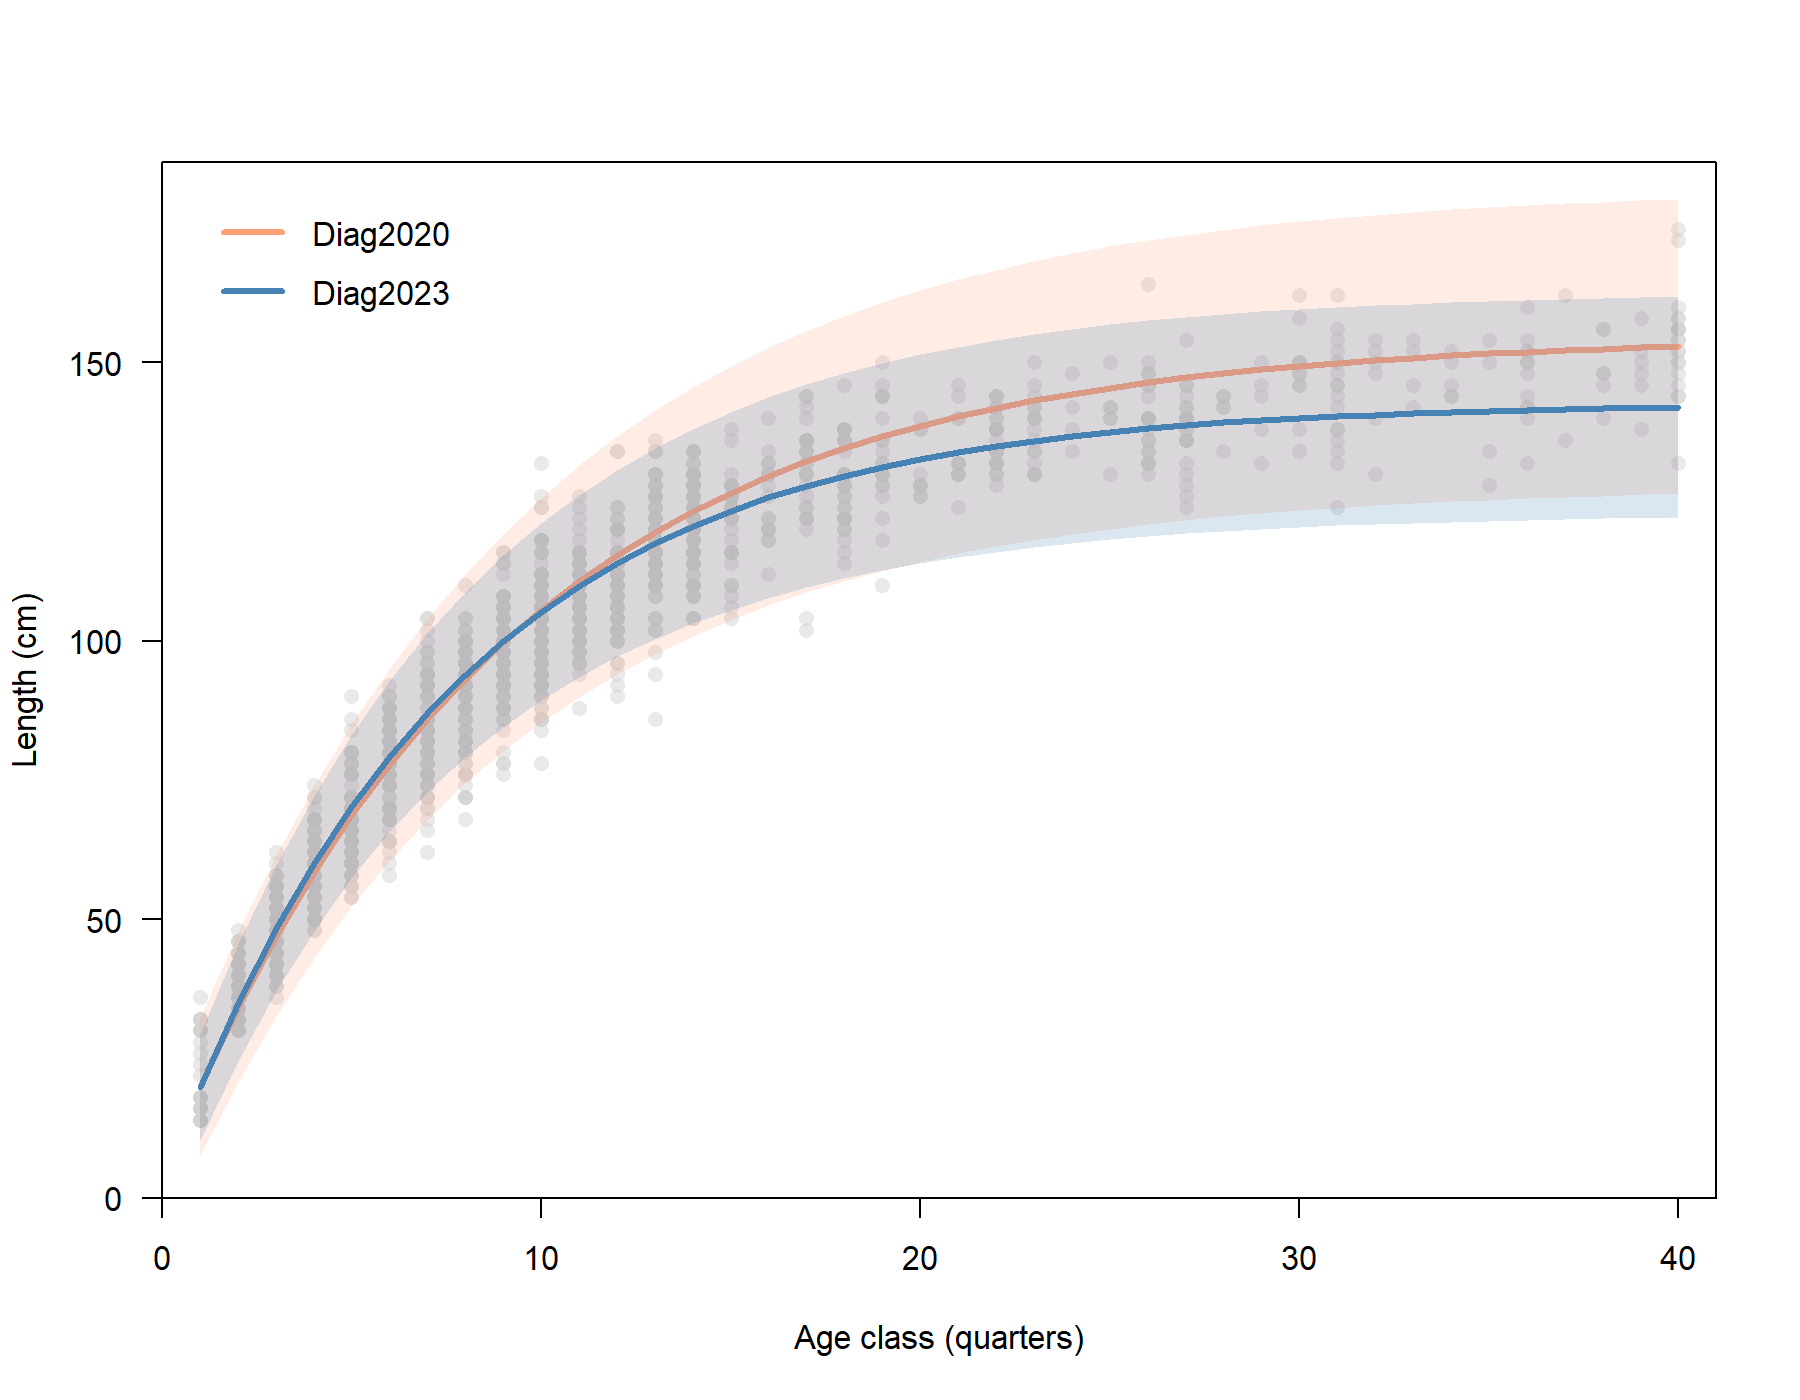
\includegraphics[width=0.9\textwidth]{growth_curve.png}\\
  ~\hspace{14mm}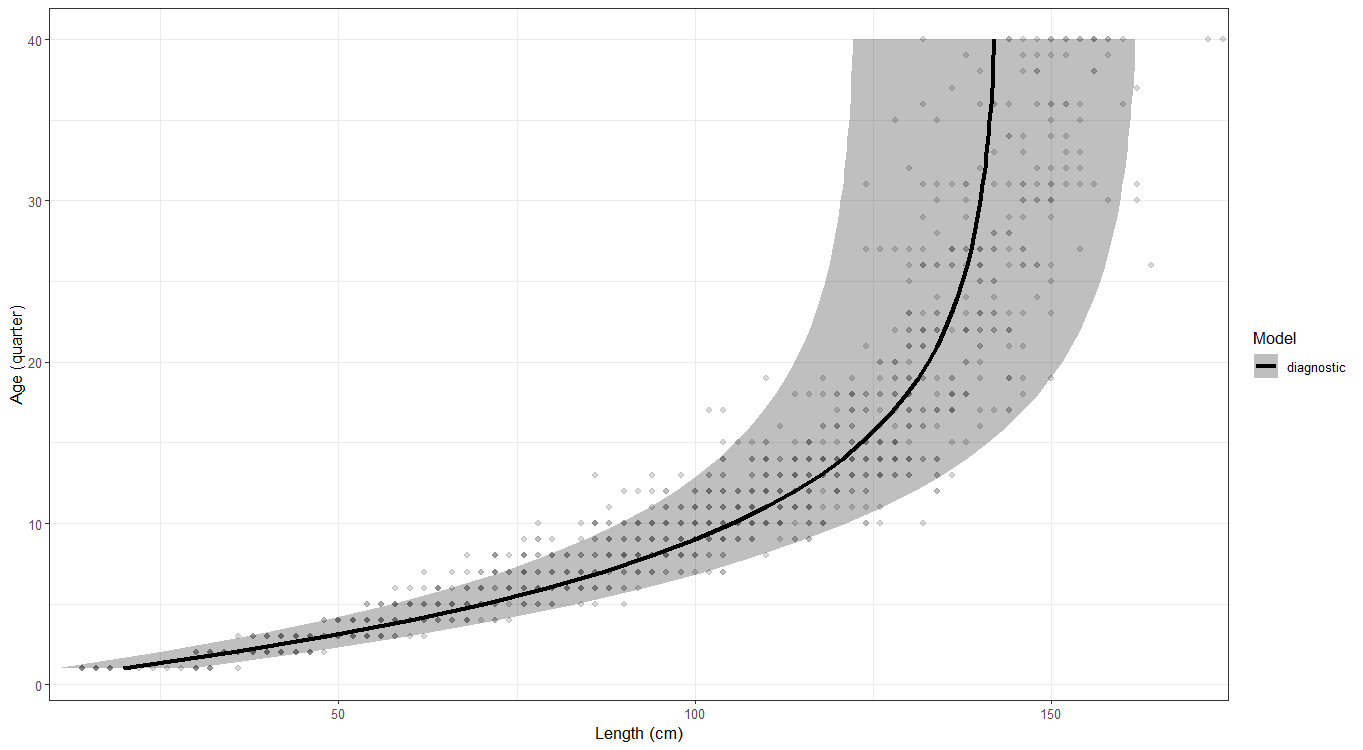
\includegraphics[width=0.9\textwidth]{growth_CAAL.png}
  \caption{Growth curves compared between the 2020 diagnostic model and 2023 diagnostic model (top). Transposed version 2023 diagnostic model for conditional-age-at-length, vertical distribution of the points indicates the distributions of observed ages for each length (bottom). Points are age-length samples for the 2023 assessment. \label{fig:growth_curve}}
\end{figure}
\clearpage

\newpage
\begin{figure}[!ht]
  \centering
  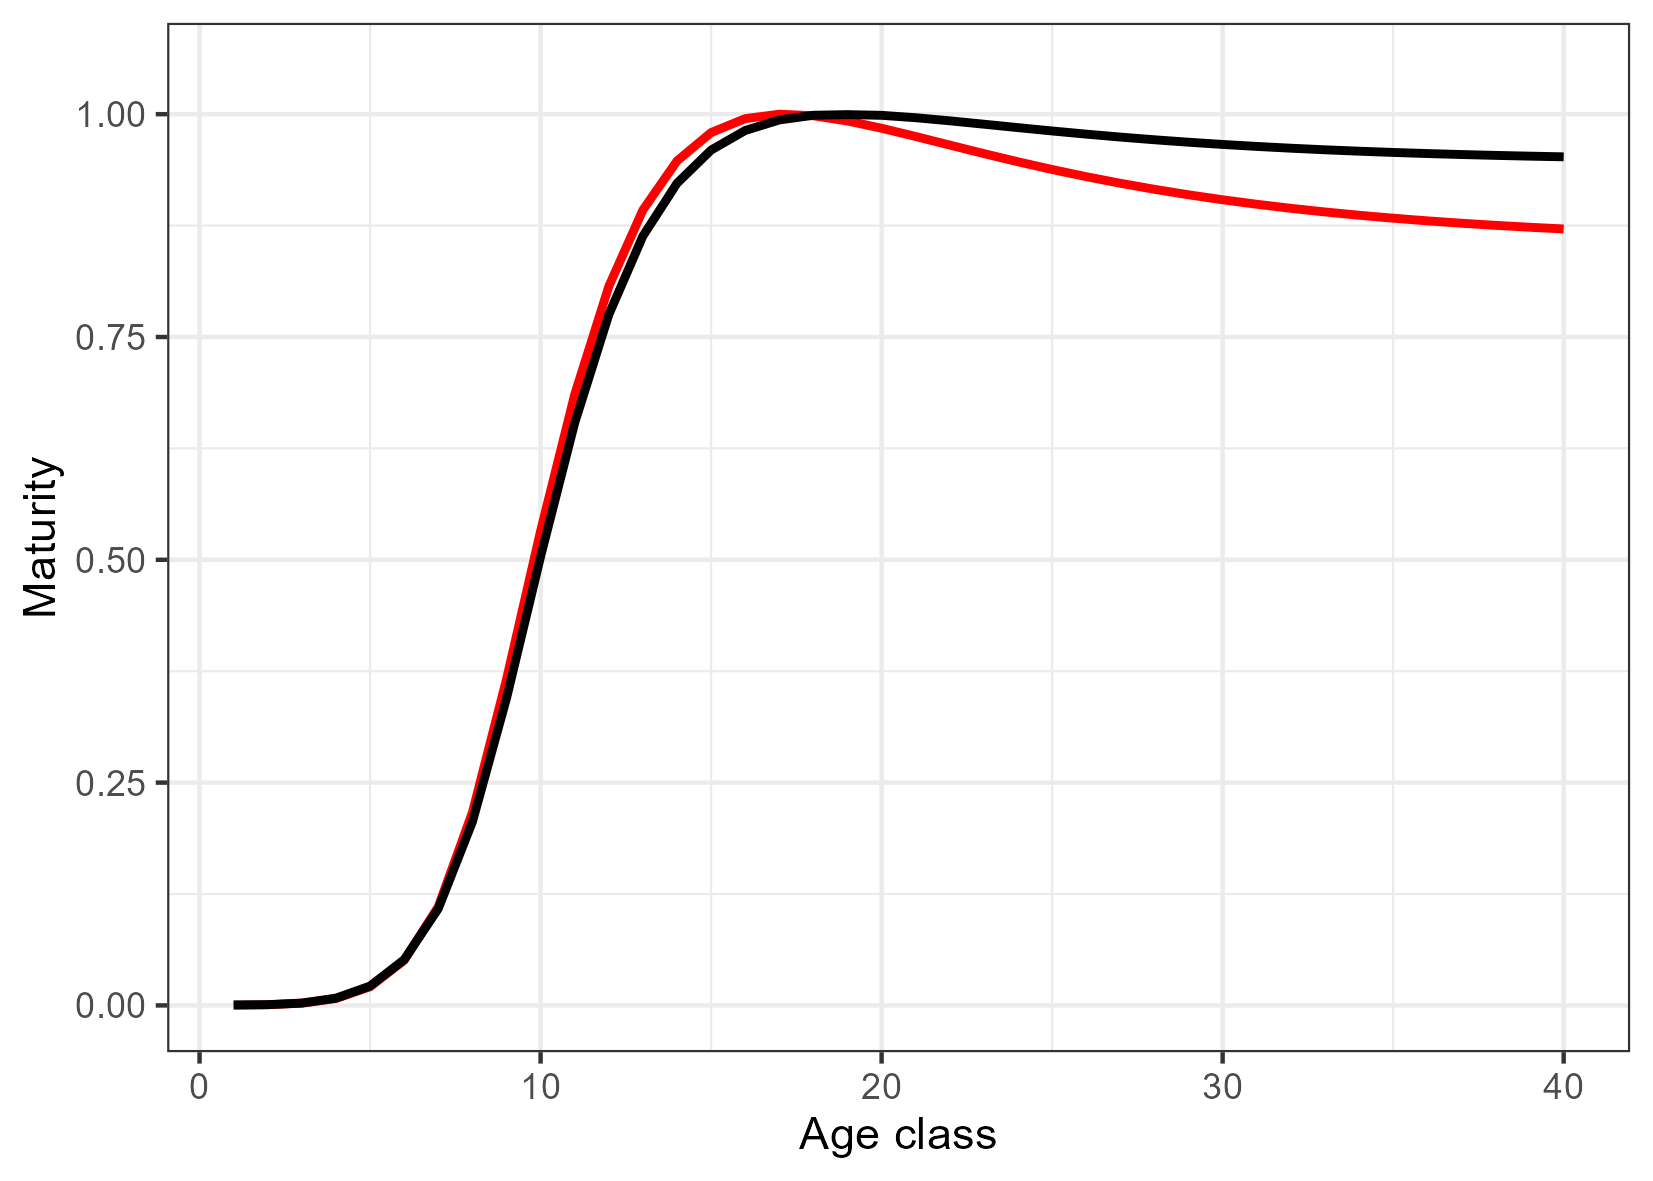
\includegraphics[width=0.8\textwidth]{maturity_ogive.png}
  \caption{Maturity-at-age ogive compared between 2020 diagnostic model (red) and 2023 diagnostic model (black). \label{fig:maturity_ogive}}
\end{figure}
\clearpage

\newpage
\begin{figure}[!ht]
  \centering
  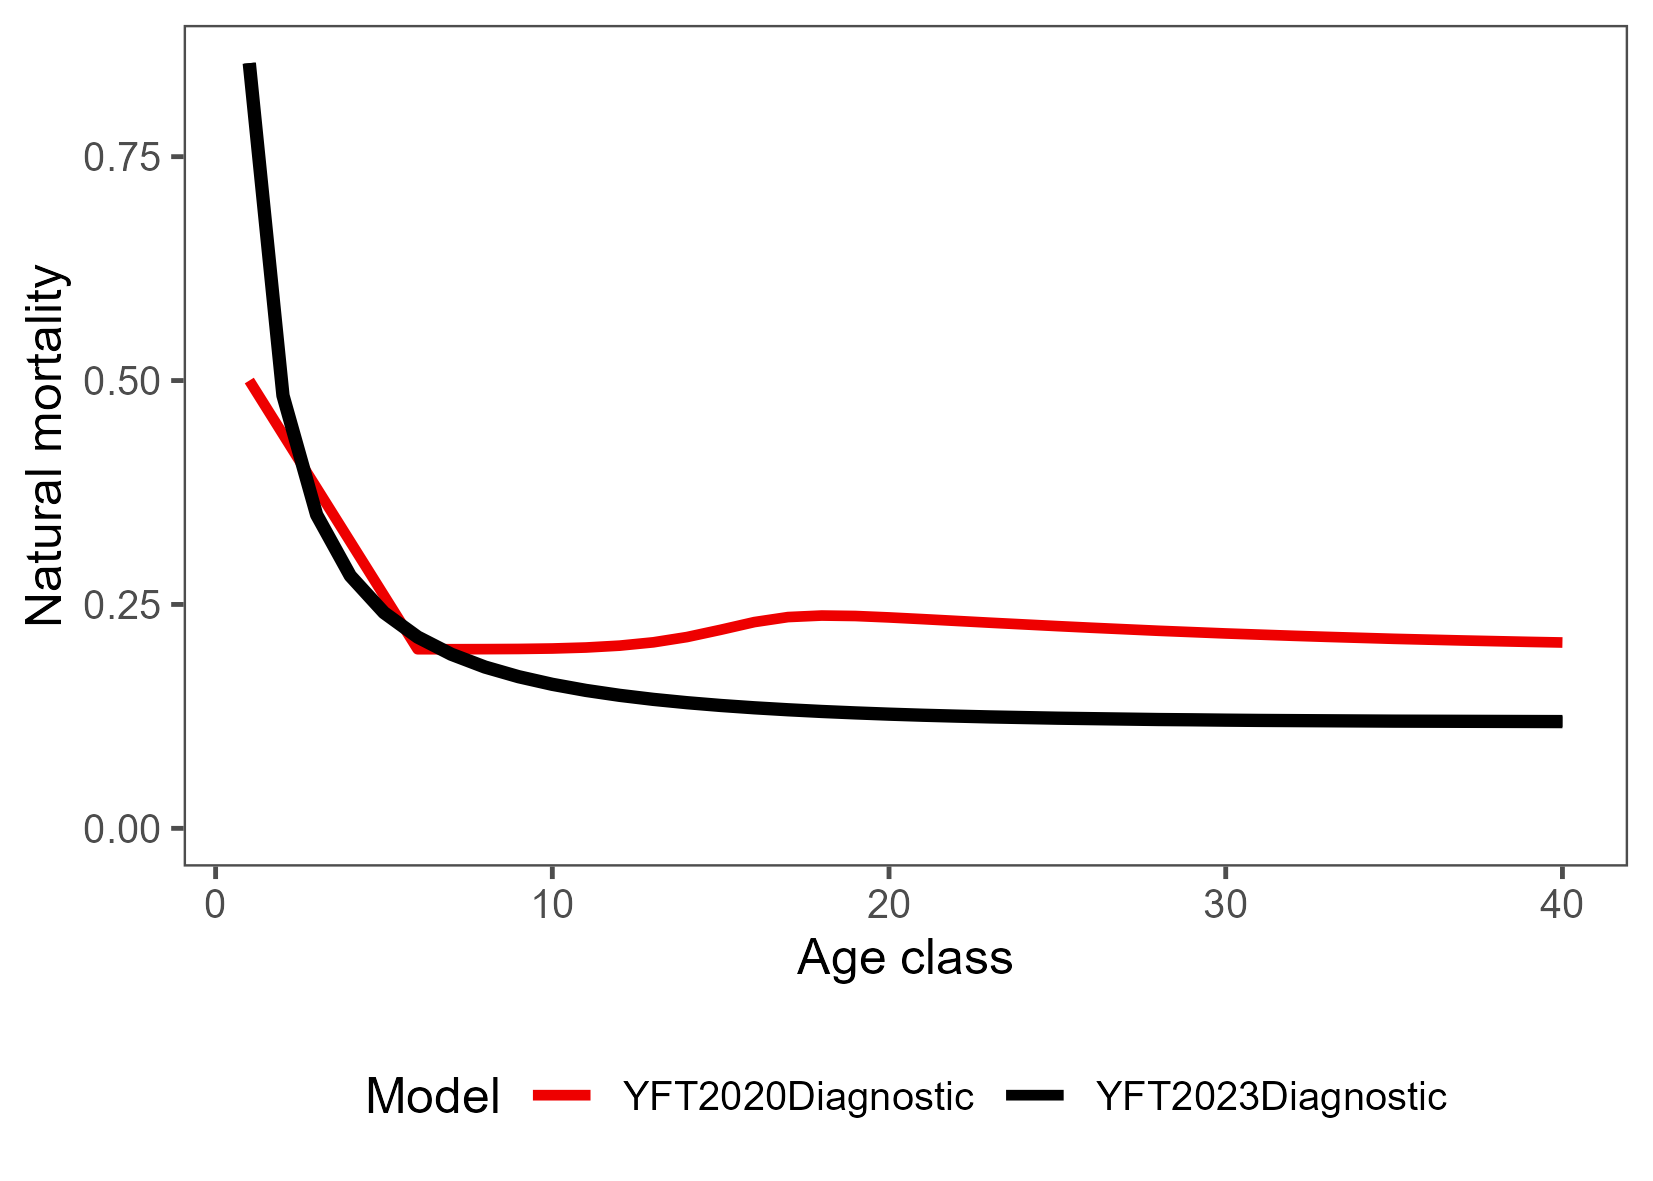
\includegraphics[width=0.8\textwidth]{natm_at_age.png}
  \caption{Natural mortality-at-age (quarters) for the 2020 diagnostic model (red) and the 2023 diagnostic model (black). \label{fig:natm_at_age}}
\end{figure}
\clearpage

\newpage
\begin{landscape}
  \begin{figure}[!ht]
    \centering
    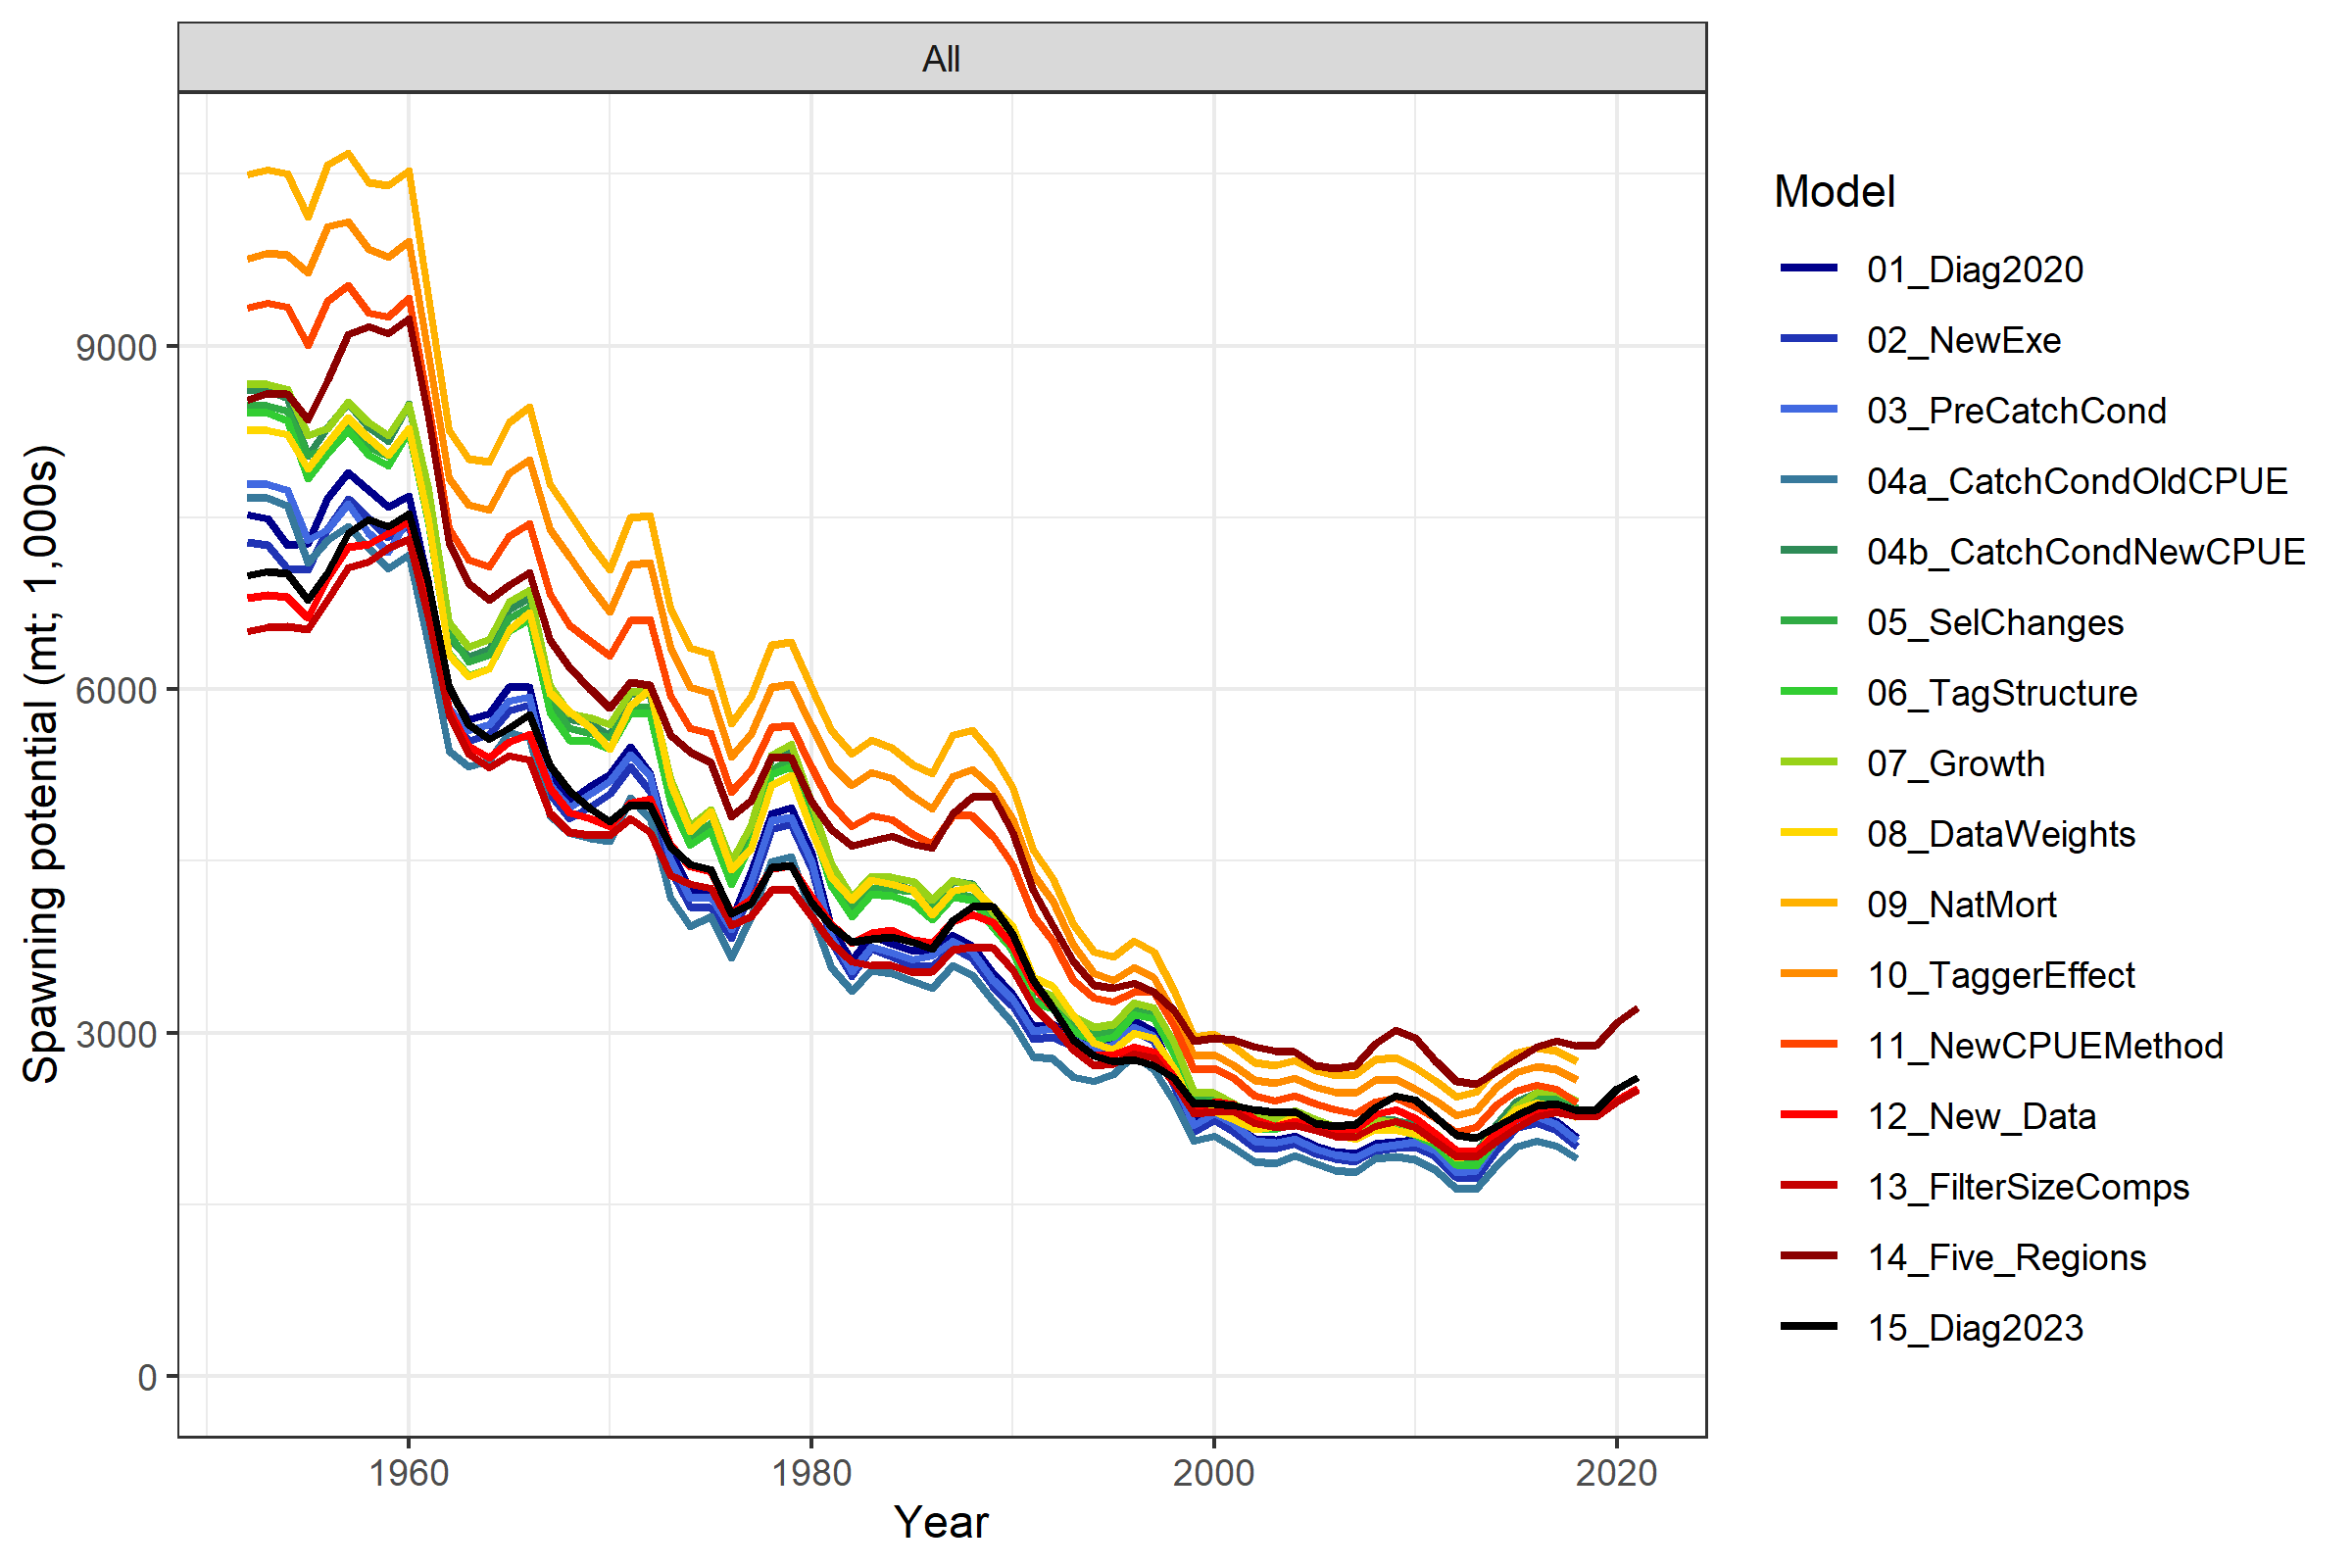
\includegraphics[width=1.2\textwidth]{stepwise_biomass.png}
    \caption{Estimated spawning potential, \sbt, trajectories for each of the main steps in the stepwise model runs, final diagnostic model is black. \label{fig:stepwise_biomass}}
  \end{figure}
\end{landscape}
\clearpage

\newpage
\begin{landscape}
  \begin{figure}[!ht]
    \centering
    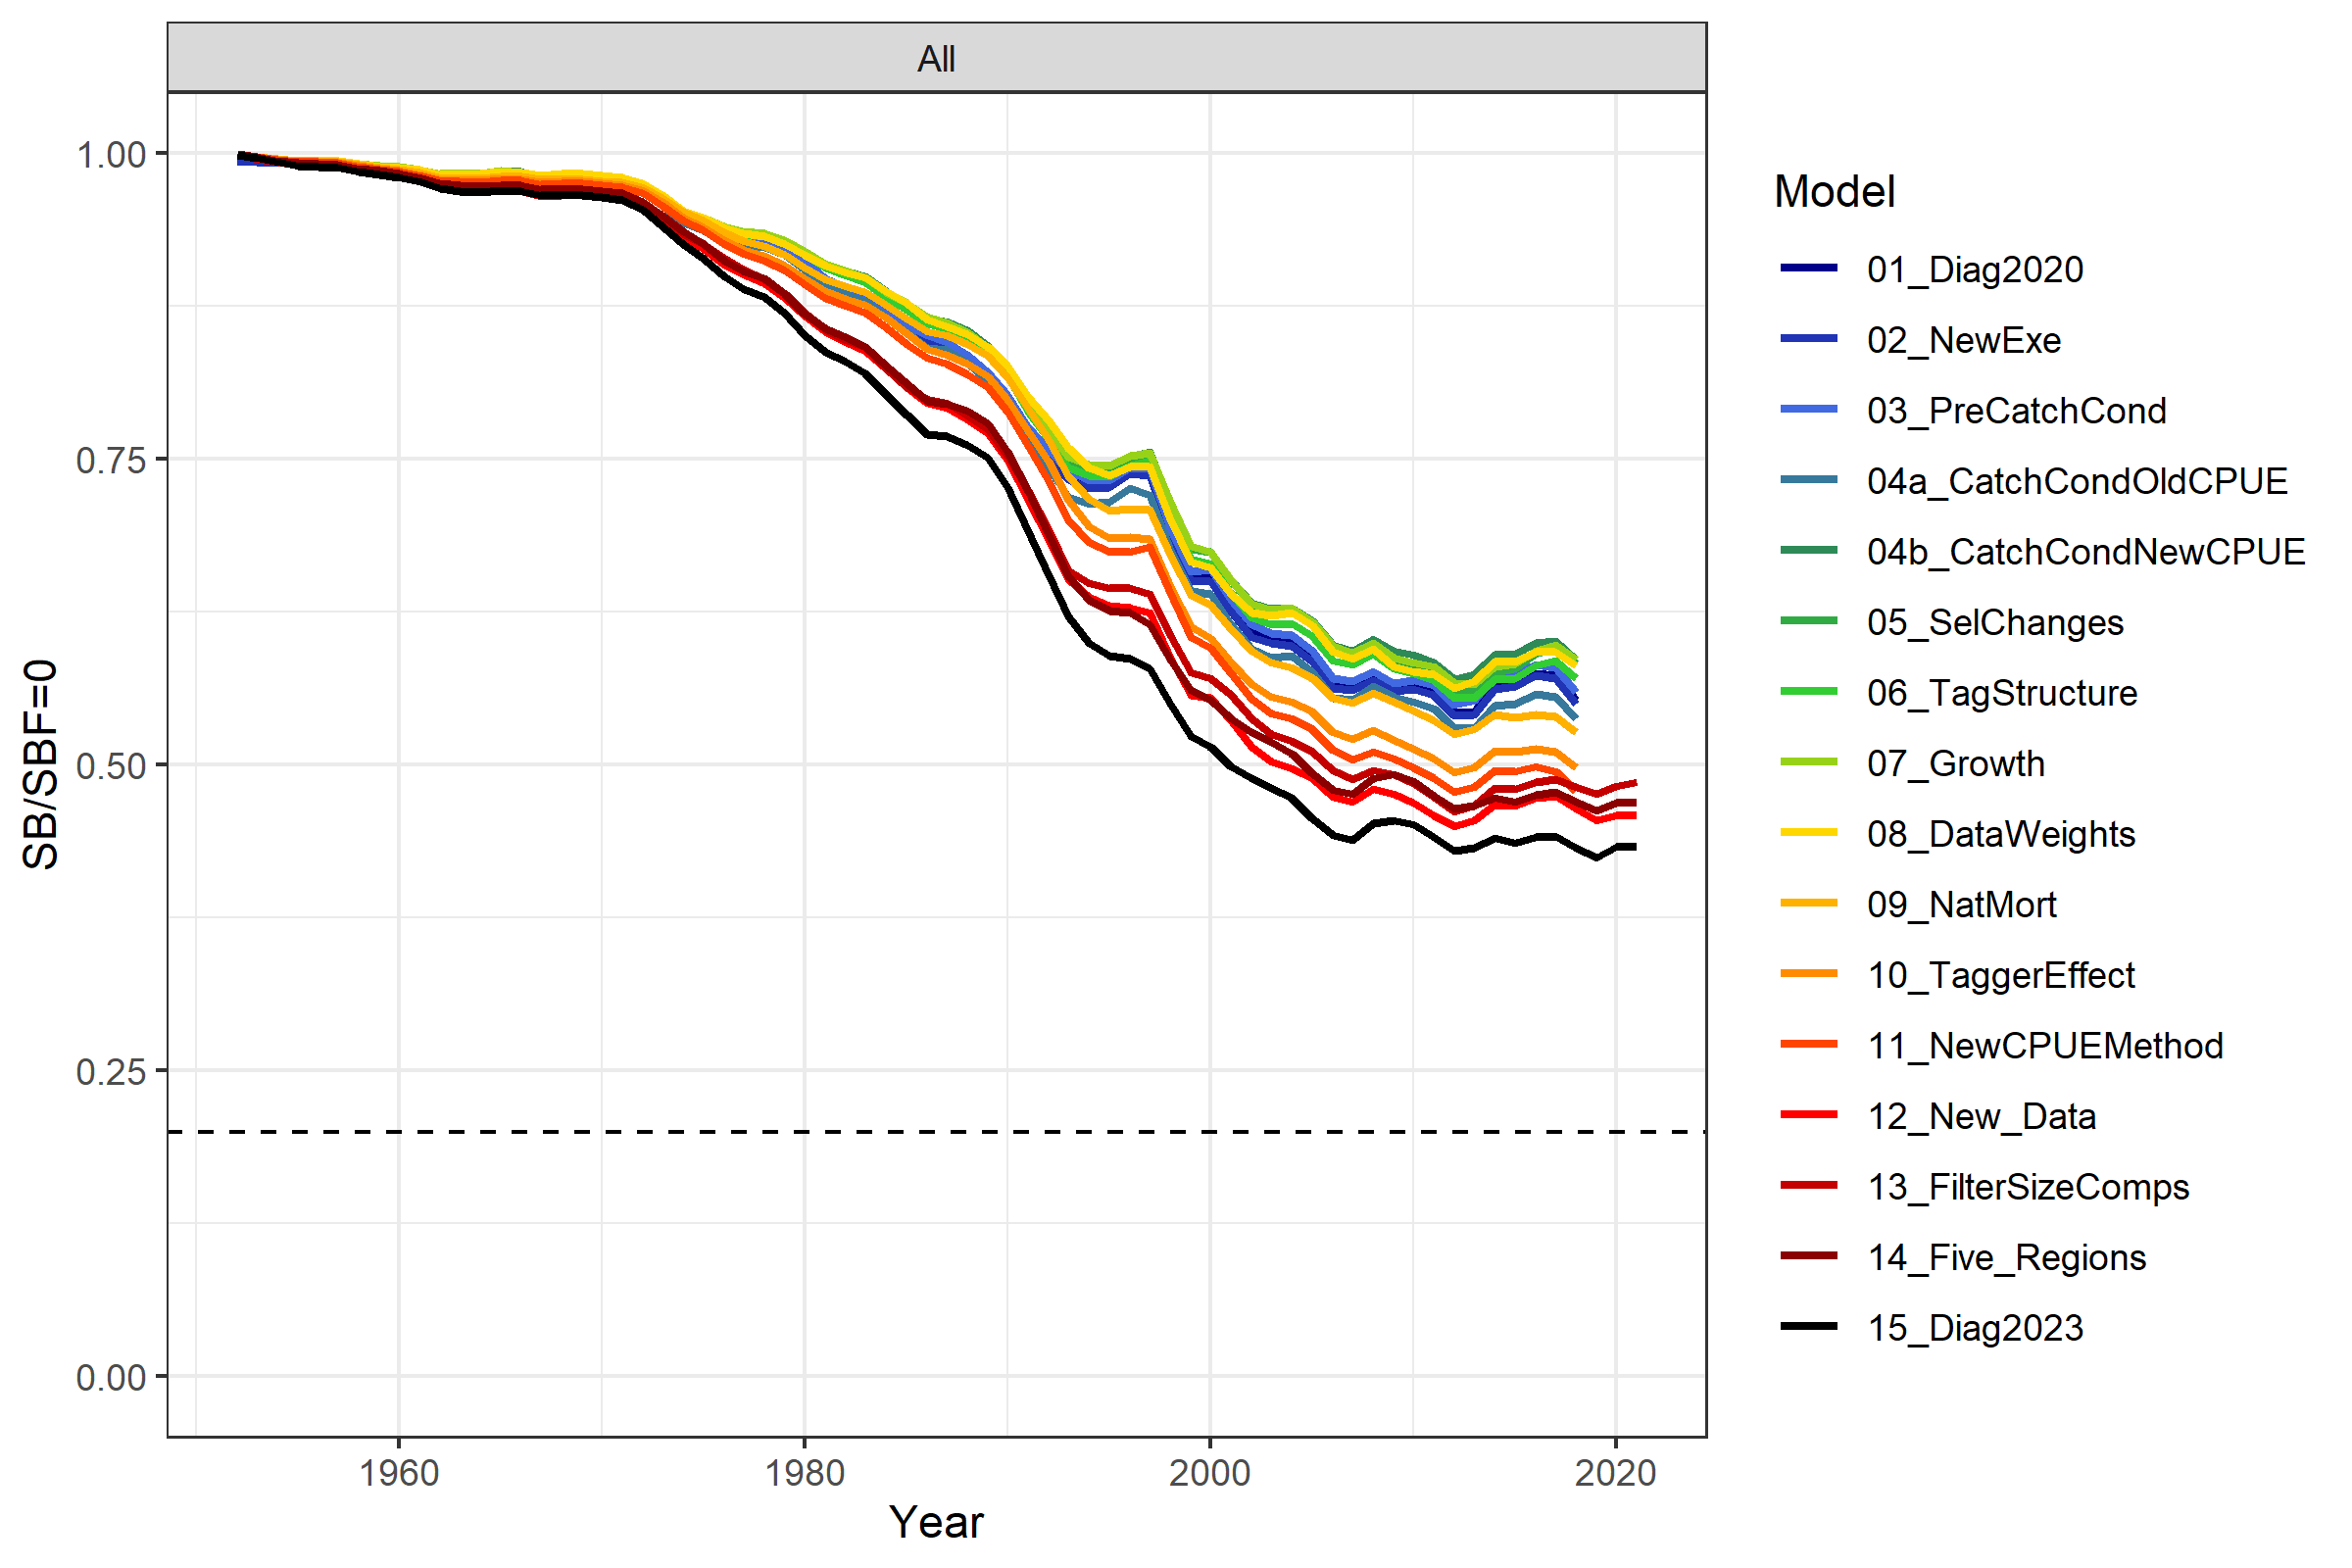
\includegraphics[width=1.2\textwidth]{stepwise_depletion.png}
    \caption{Estimated dynamic spawning depletion, \sbtsbfo, trajectories for each of the main steps in the stepwise model runs, final diagnostic model is black. \label{fig:stepwise_depletion}}
  \end{figure}
\end{landscape}
\clearpage

\newpage
\begin{figure}[!ht]
  \centering
  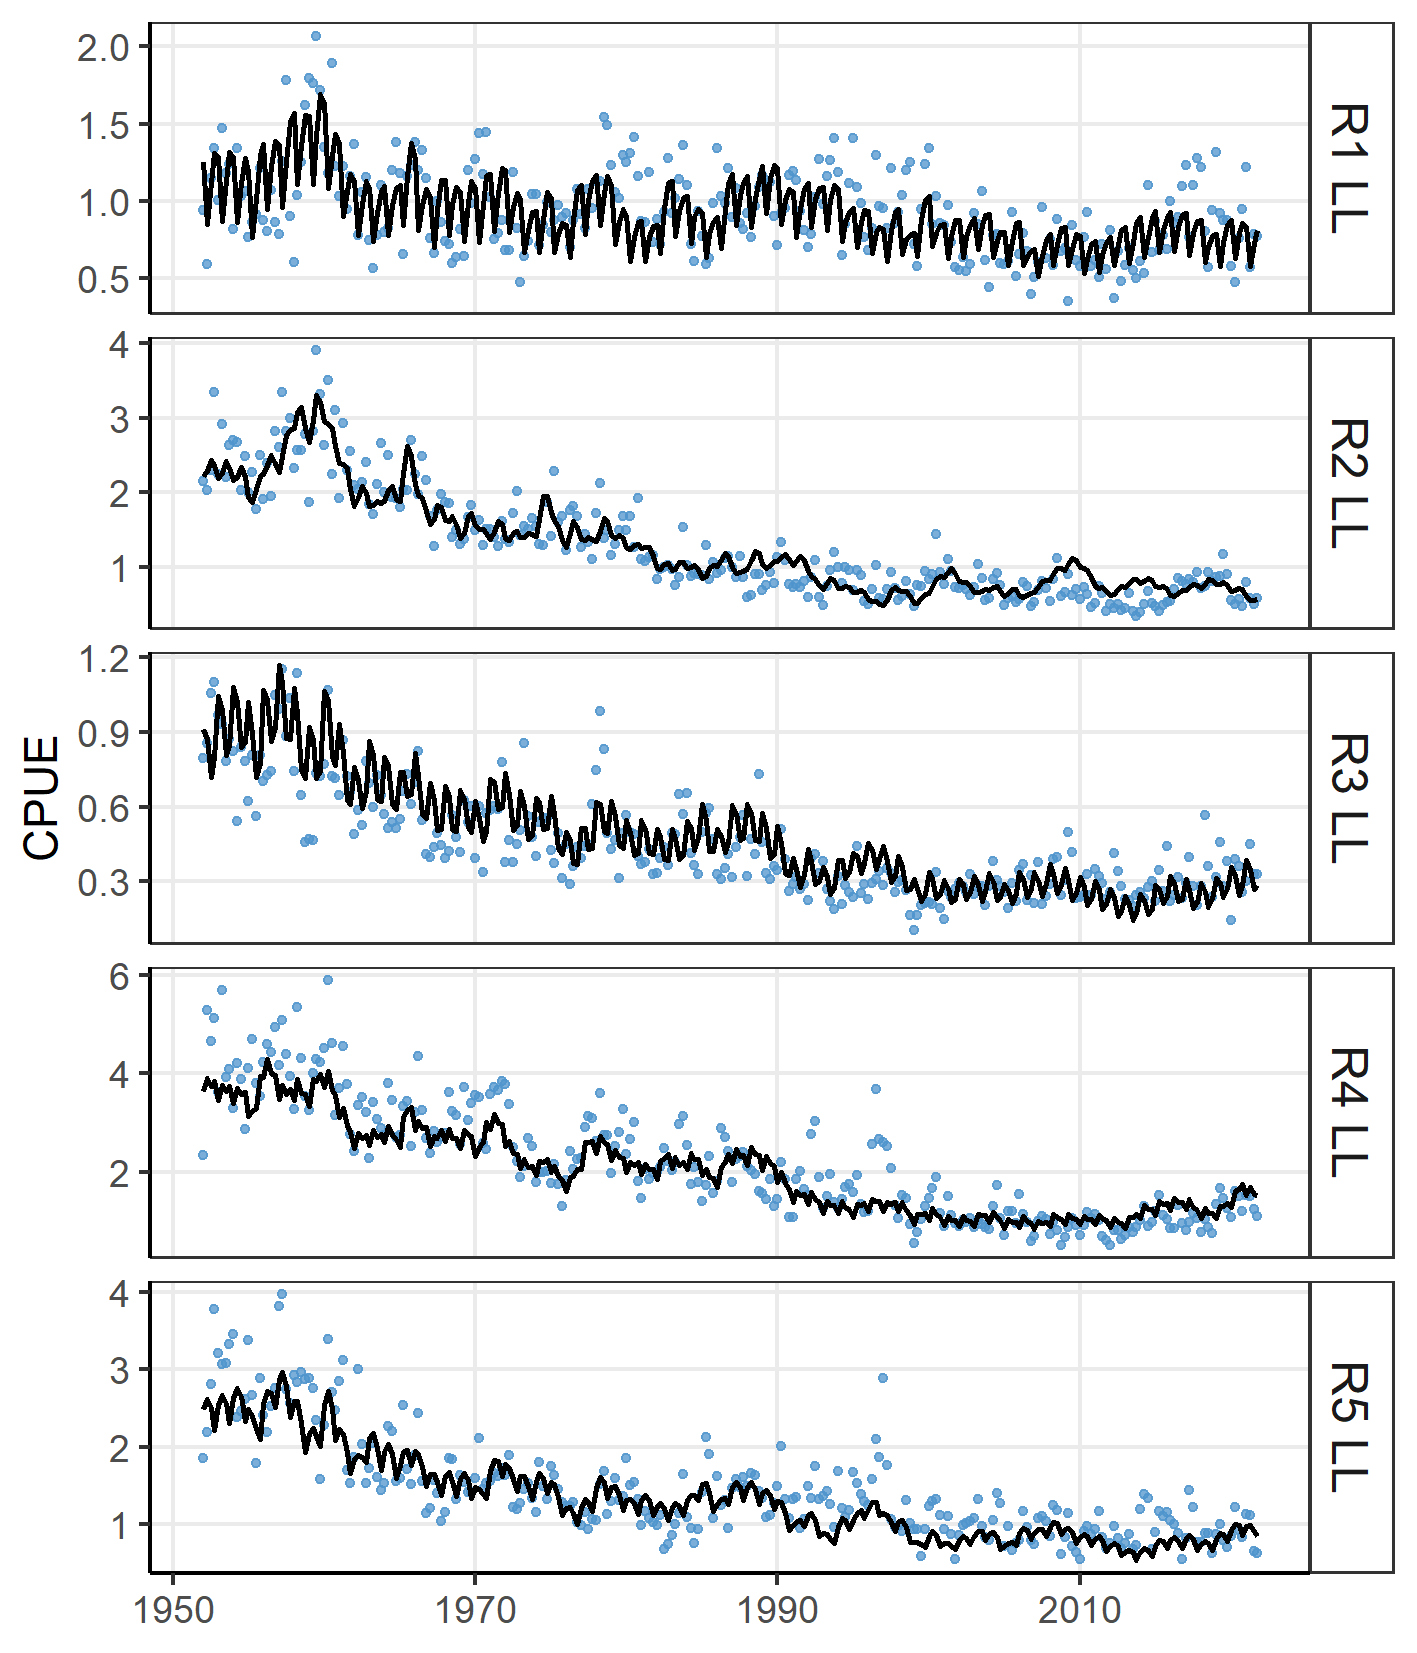
\includegraphics[width=0.9\textwidth]{cpue_fit.png}
  \caption{Comparison of model estimated (black line) and observed standardised CPUE (blue dots) for the longline index fisheries in each region. \label{fig:cpue_fit}}
\end{figure}
\clearpage

\newpage
\begin{figure}[!ht]
  \centering
  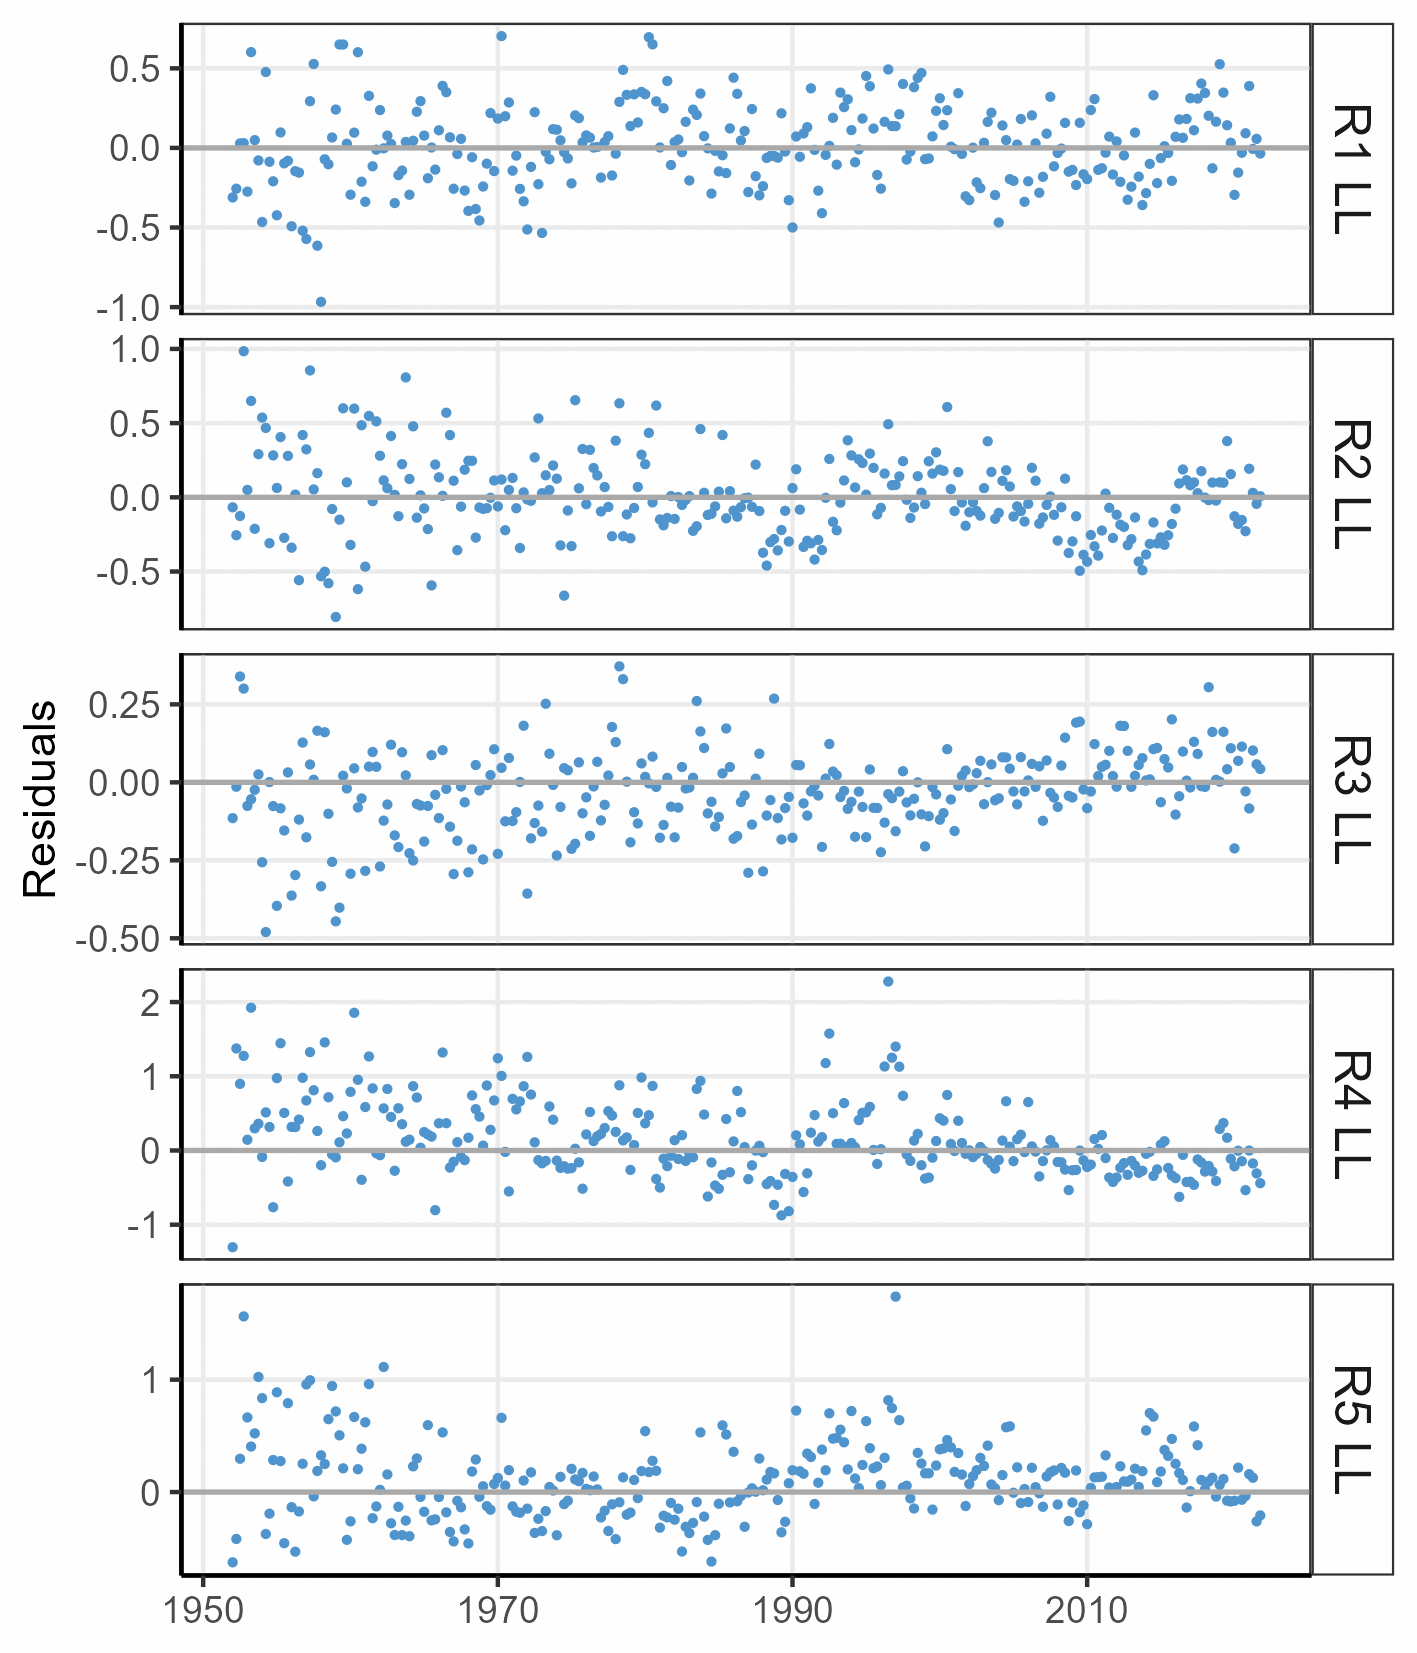
\includegraphics[width=0.9\textwidth]{cpue_resids.png}
  \caption{Plots of residuals between observed and predicted standardised CPUE for the longline index fisheries in each region.  \label{fig:cpue_resids}}
\end{figure}
\clearpage

\newpage
\begin{figure}[!ht]
  \centering
  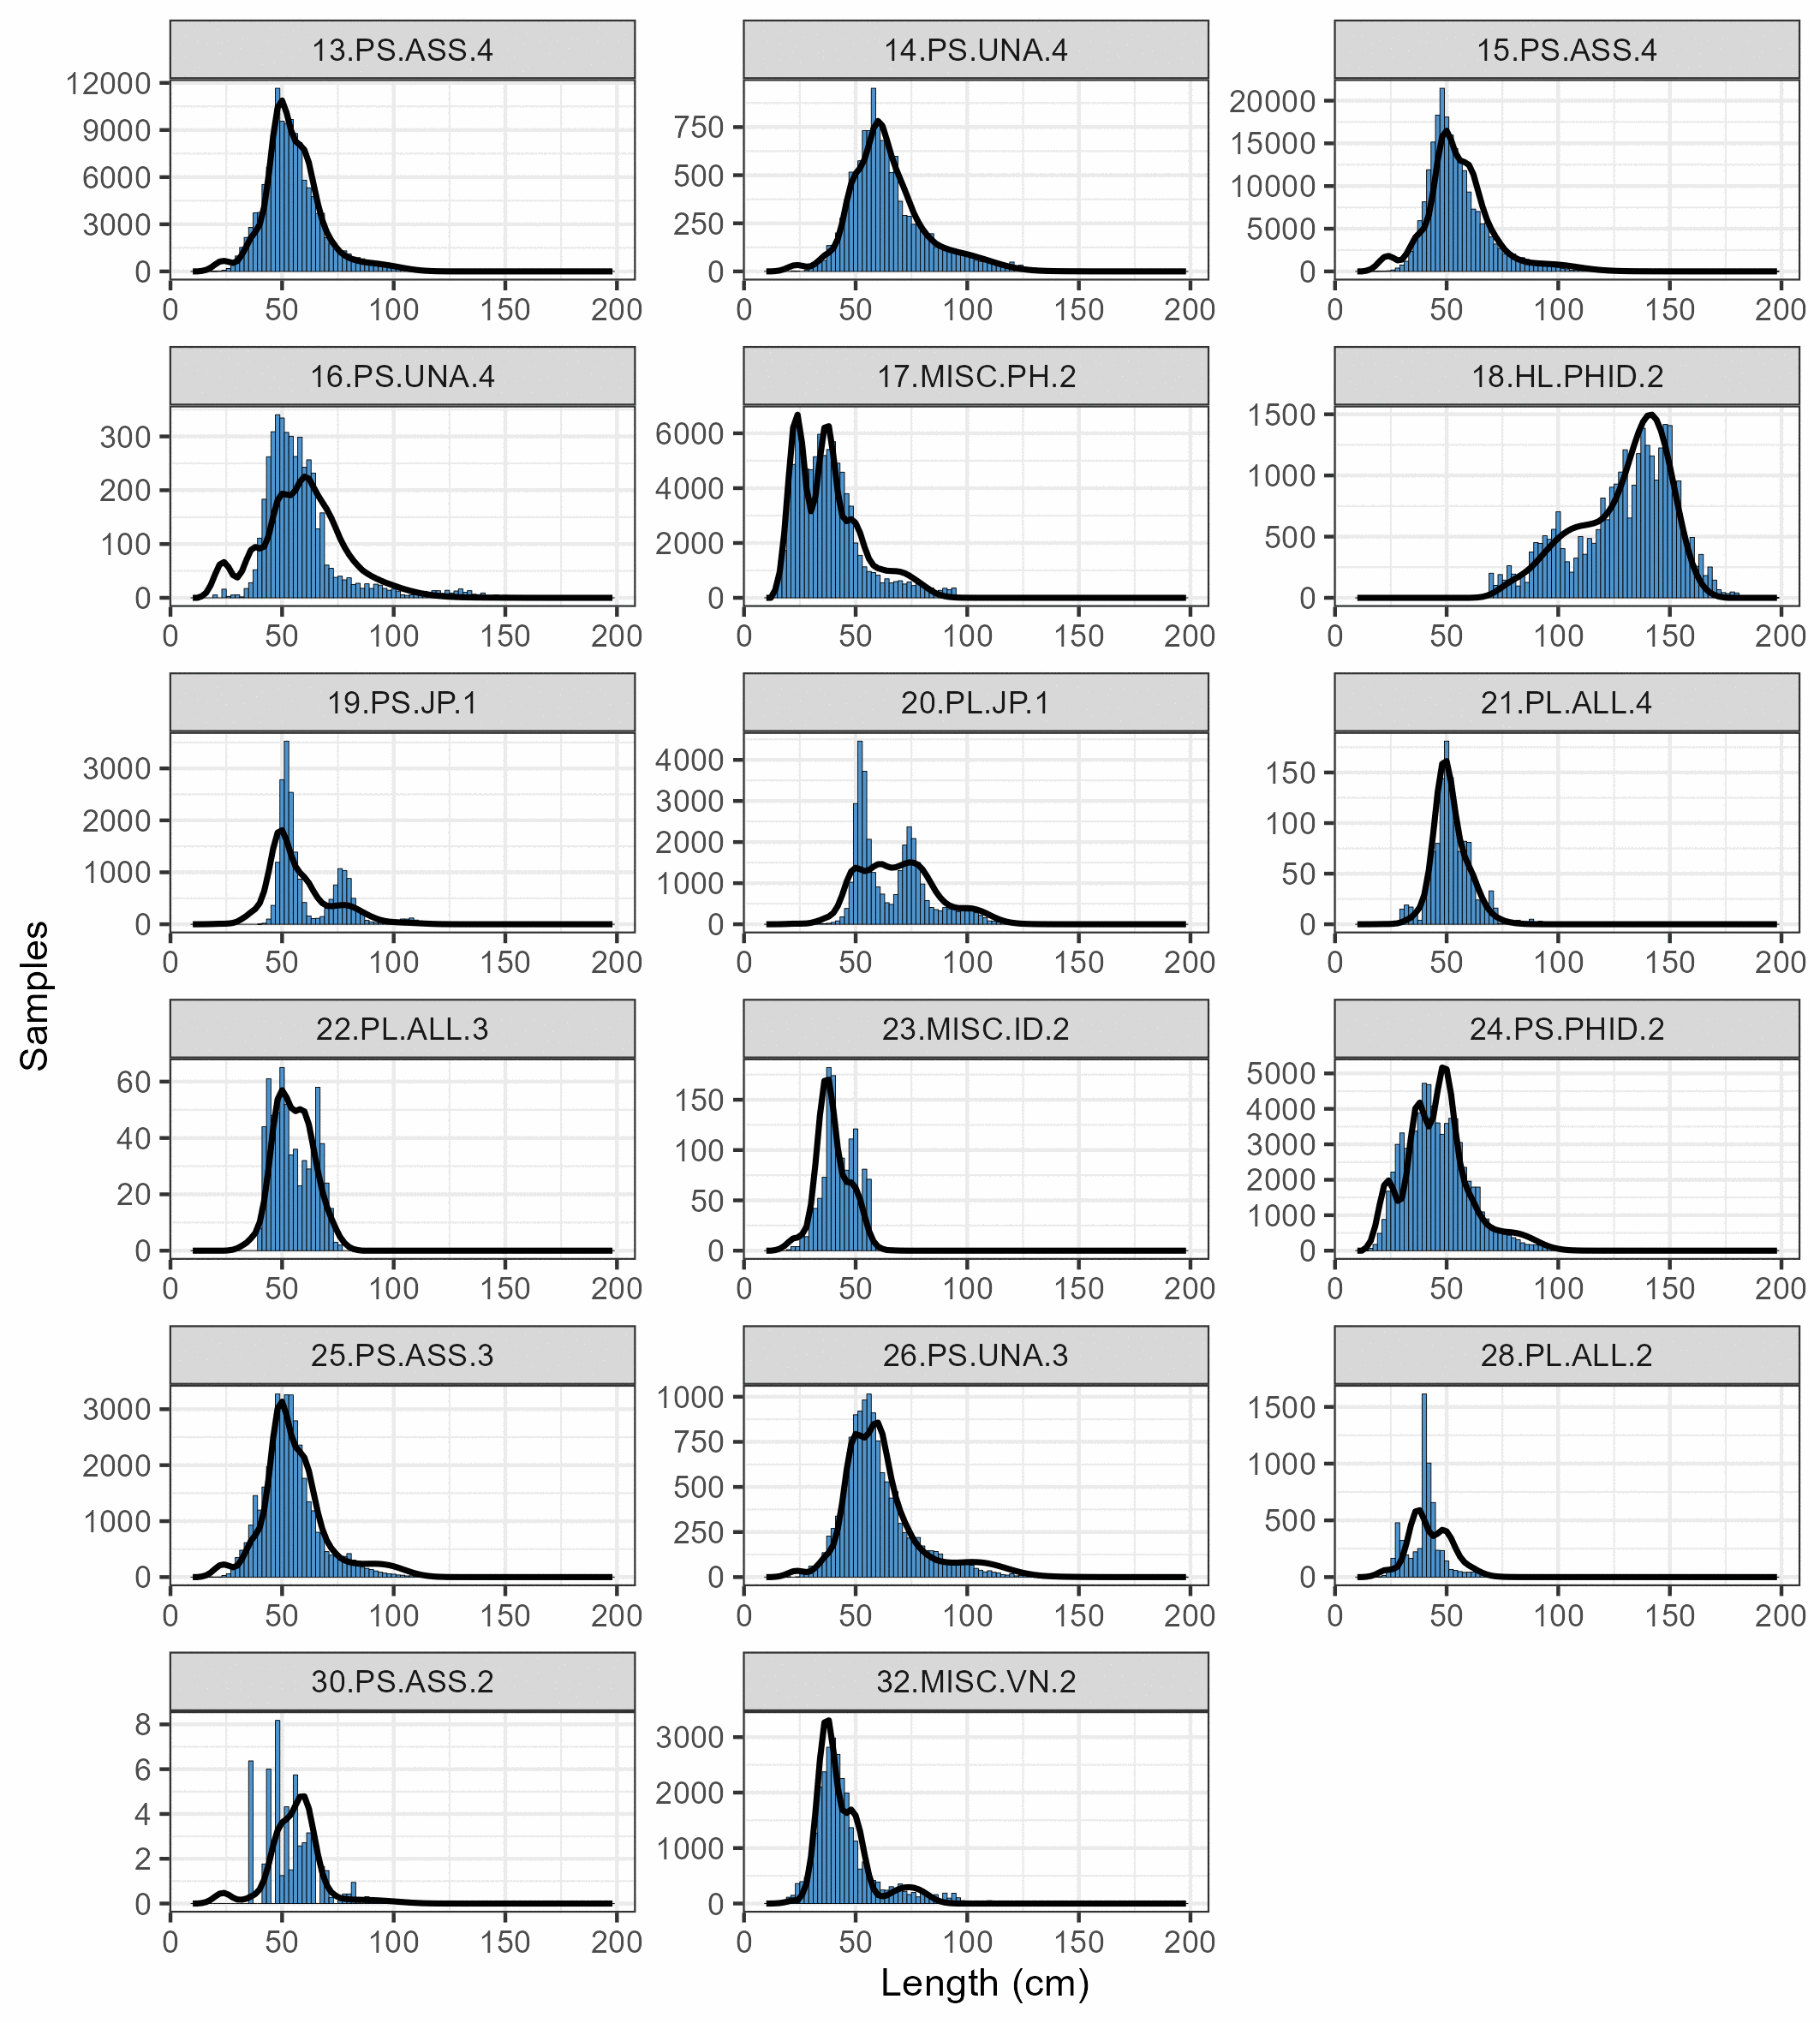
\includegraphics[width=\textwidth]{length_fit_aggregated.png}
  \caption{Composite (all time periods combined), observed (blue histograms), and predicted (black line) length frequency for fisheries with length frequency data for the diagnostic model. \label{fig:length_fit_aggregated}}
\end{figure}
\clearpage

\newpage
\begin{figure}[!ht]
  \centering
  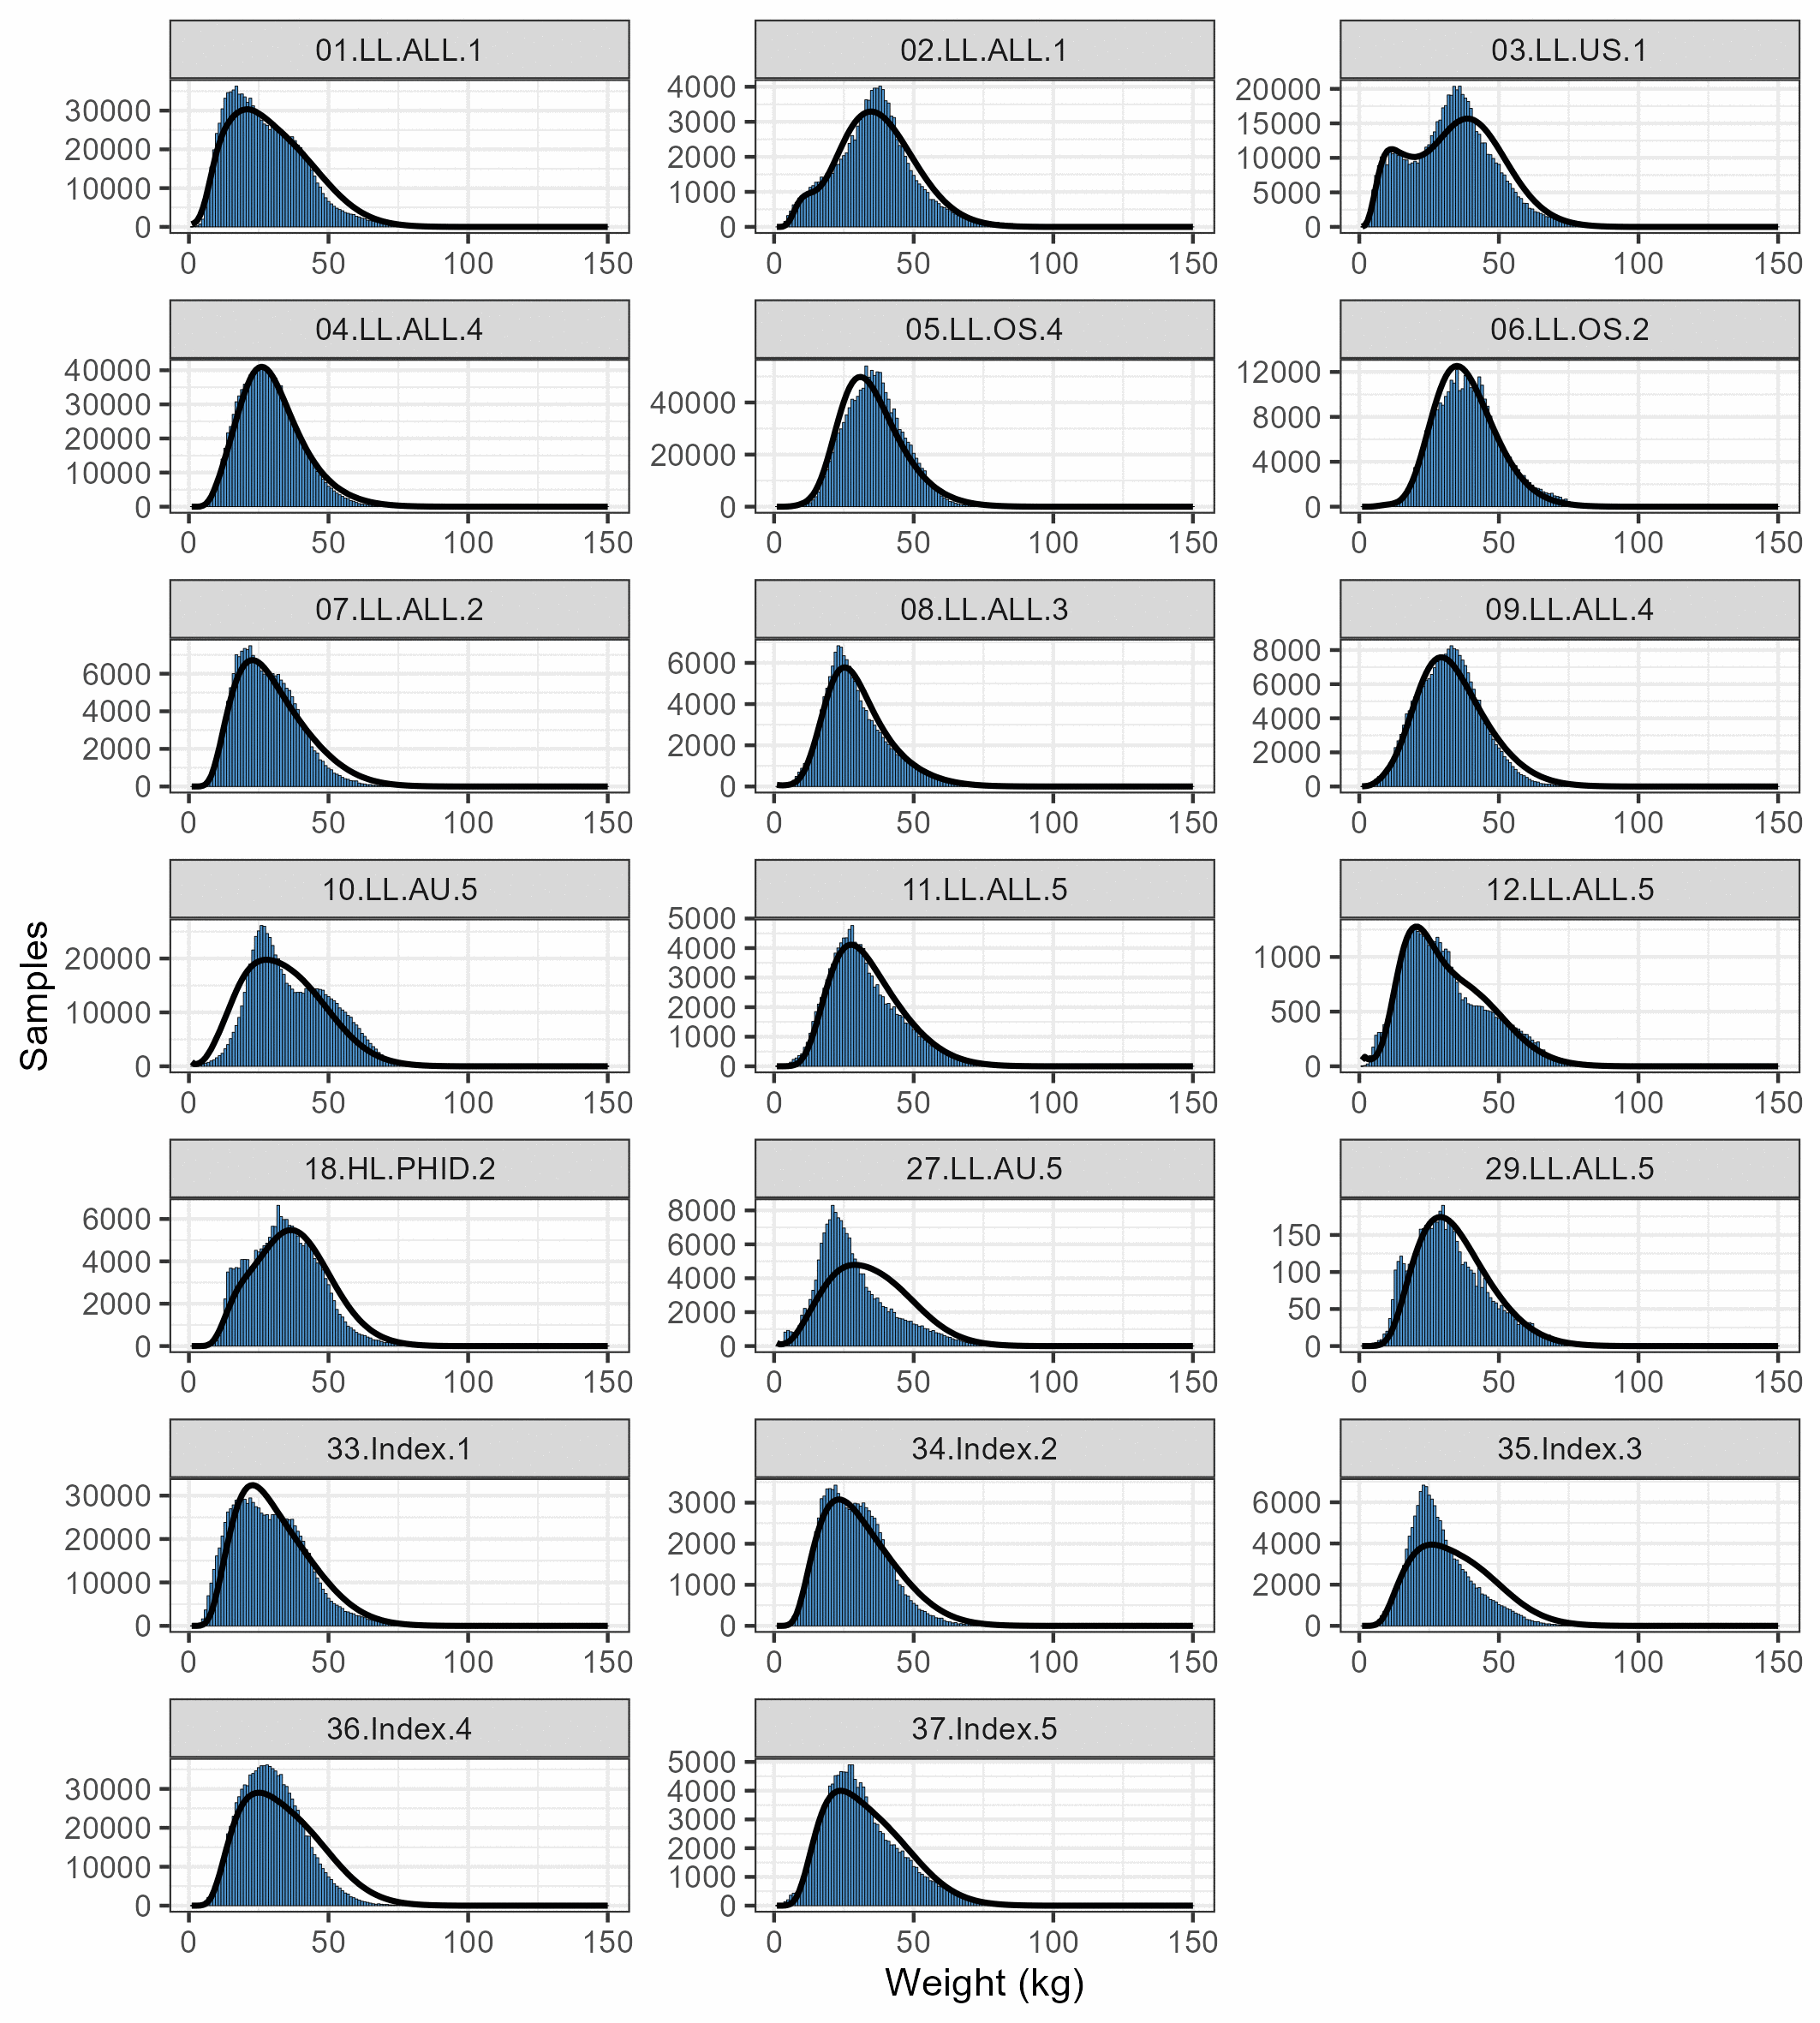
\includegraphics[width=\textwidth]{weight_fit_aggregated.png}
  \caption{Composite (all time periods combined), observed (blue histograms), and predicted (black line) weight frequency for longline fisheries for the diagnostic model. \label{fig:weight_fit_aggregated}}
\end{figure}
\clearpage

\newpage
\begin{landscape}
  \begin{figure}[!ht]
    \centering
    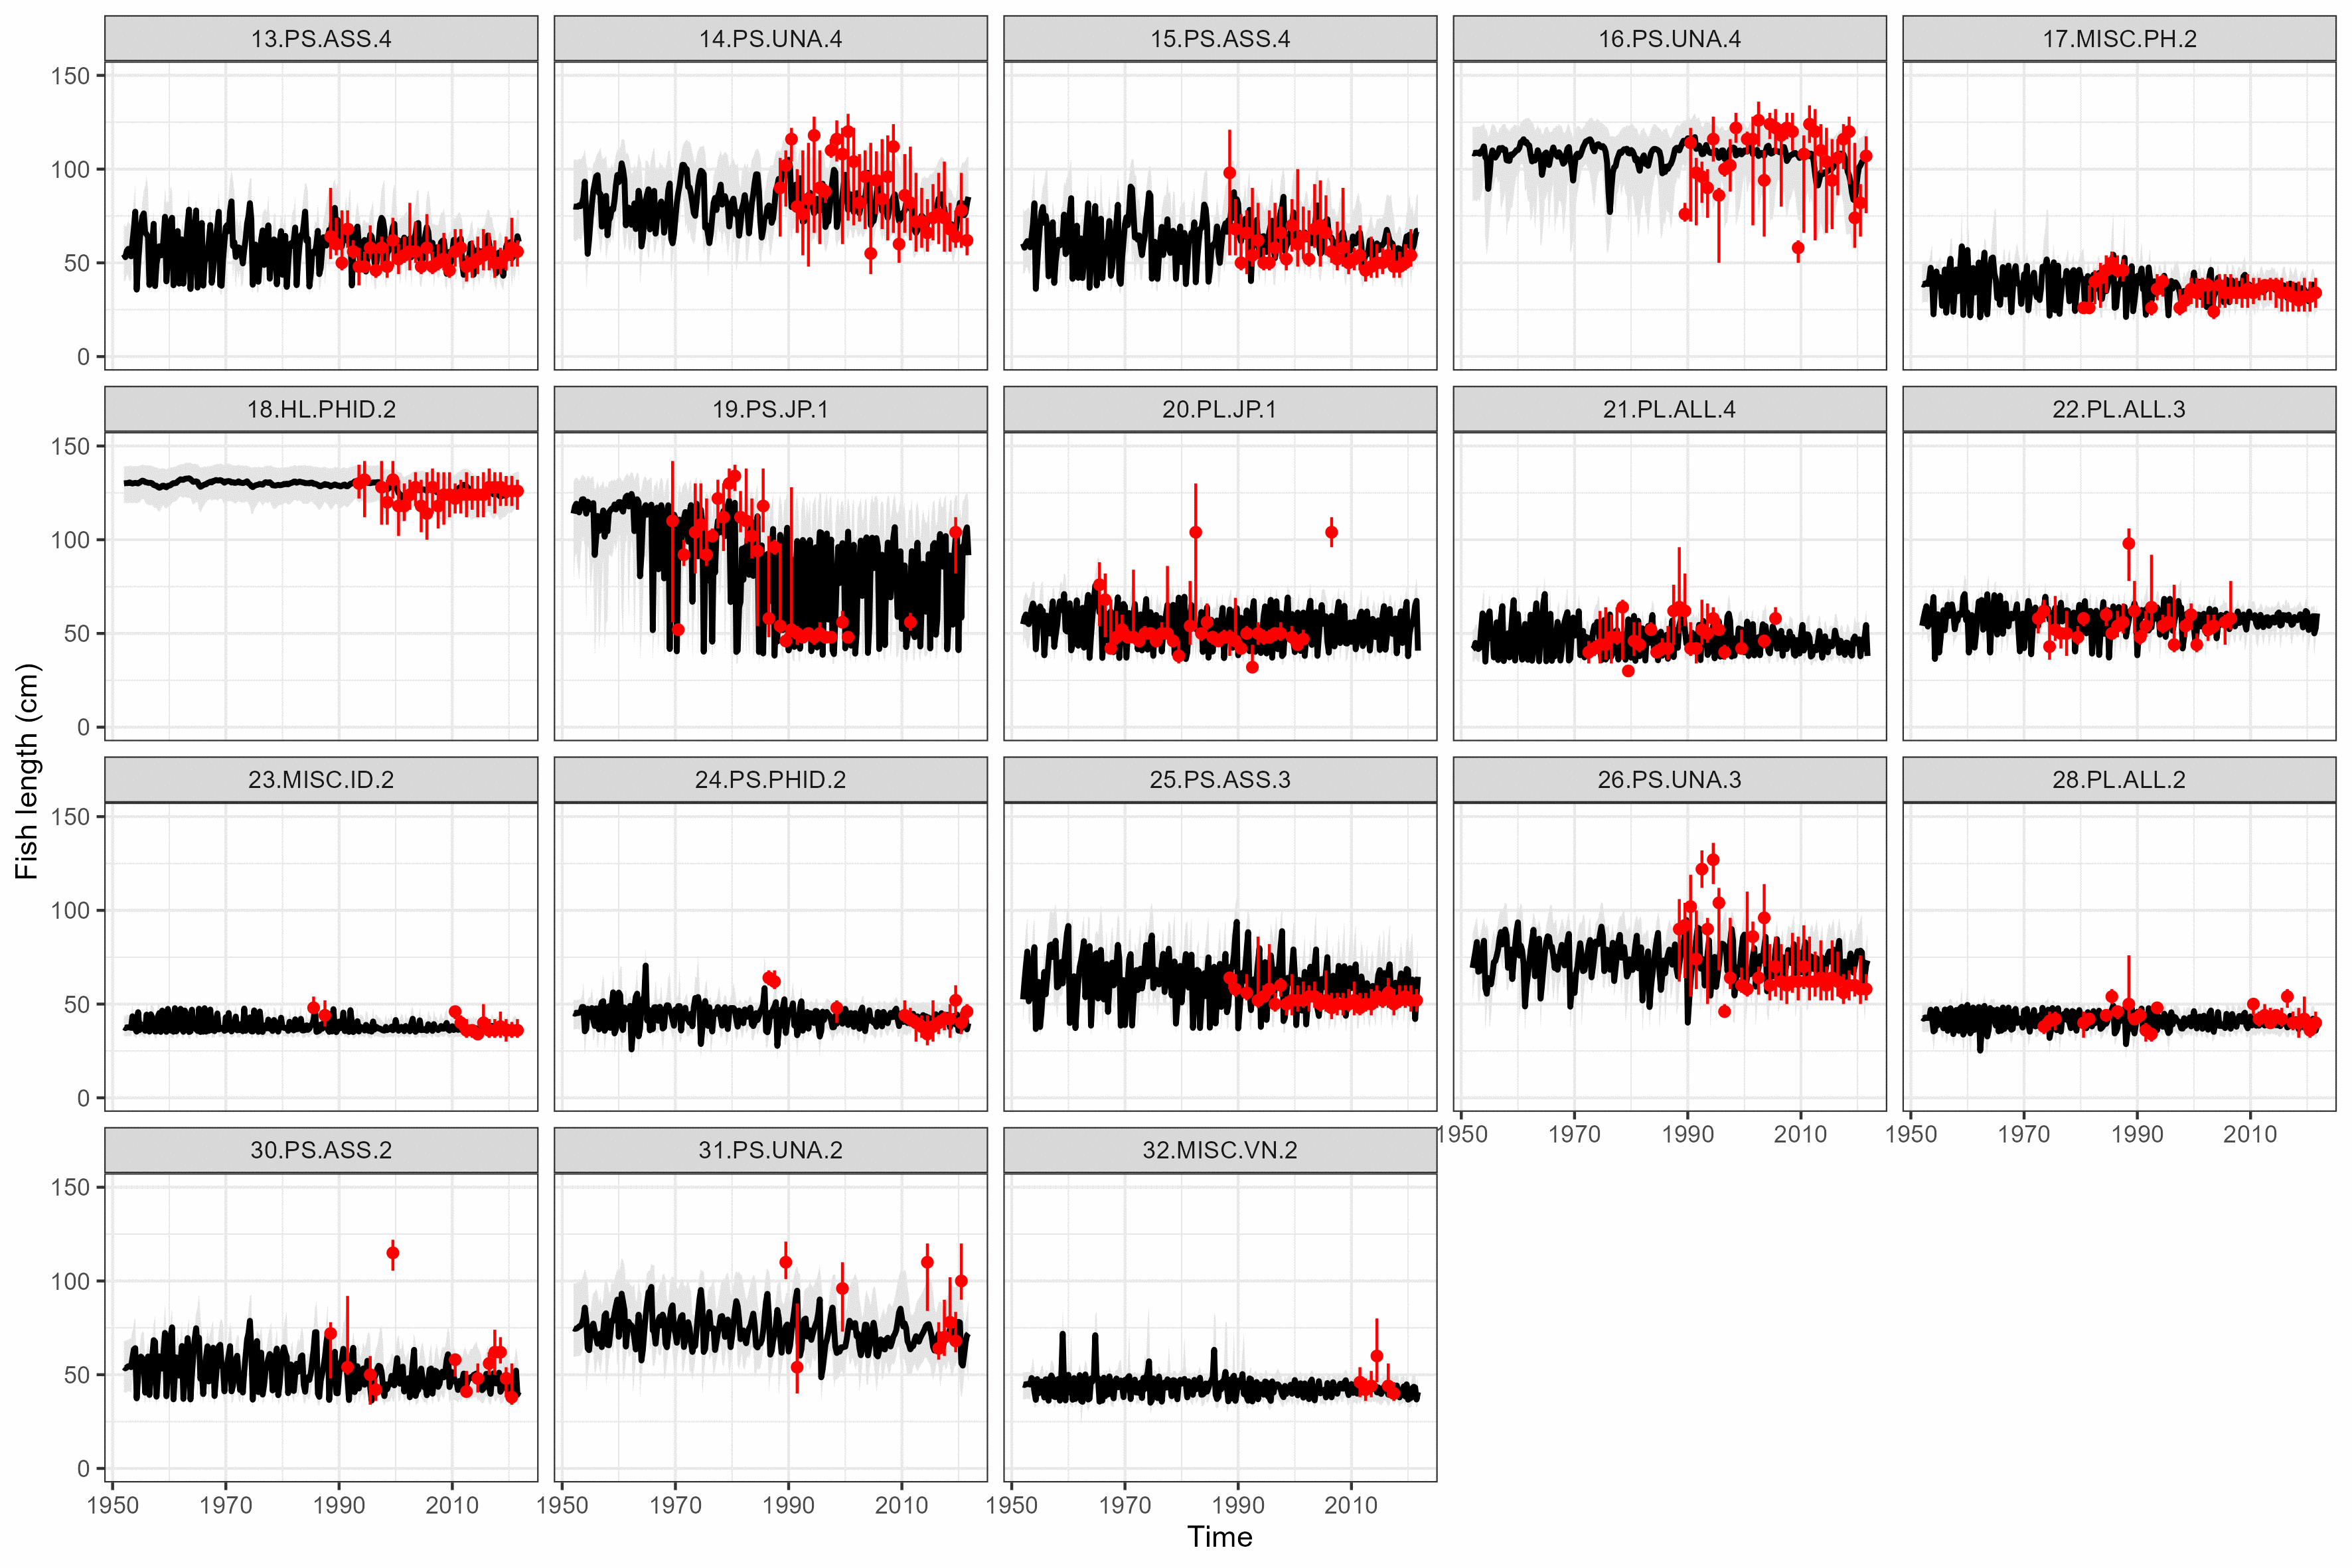
\includegraphics[width=1.3\textwidth]{length_fit_timeseries.png}
    \caption{A comparison of the observed (red points) and predicted (black line) median fish length (FL, cm) for the fisheries with length data in the diagnostic model. The uncertainty intervals (gray shading) represent the values encompassed by the 25\% and 75\% quantiles. Sampling data are by quarter and only length samples more than 30 fish per quarter are plotted. \label{fig:length_fit_timeseries}}
  \end{figure}
\end{landscape}
\clearpage

\newpage
\begin{landscape}
  \begin{figure}[!ht]
    \centering
    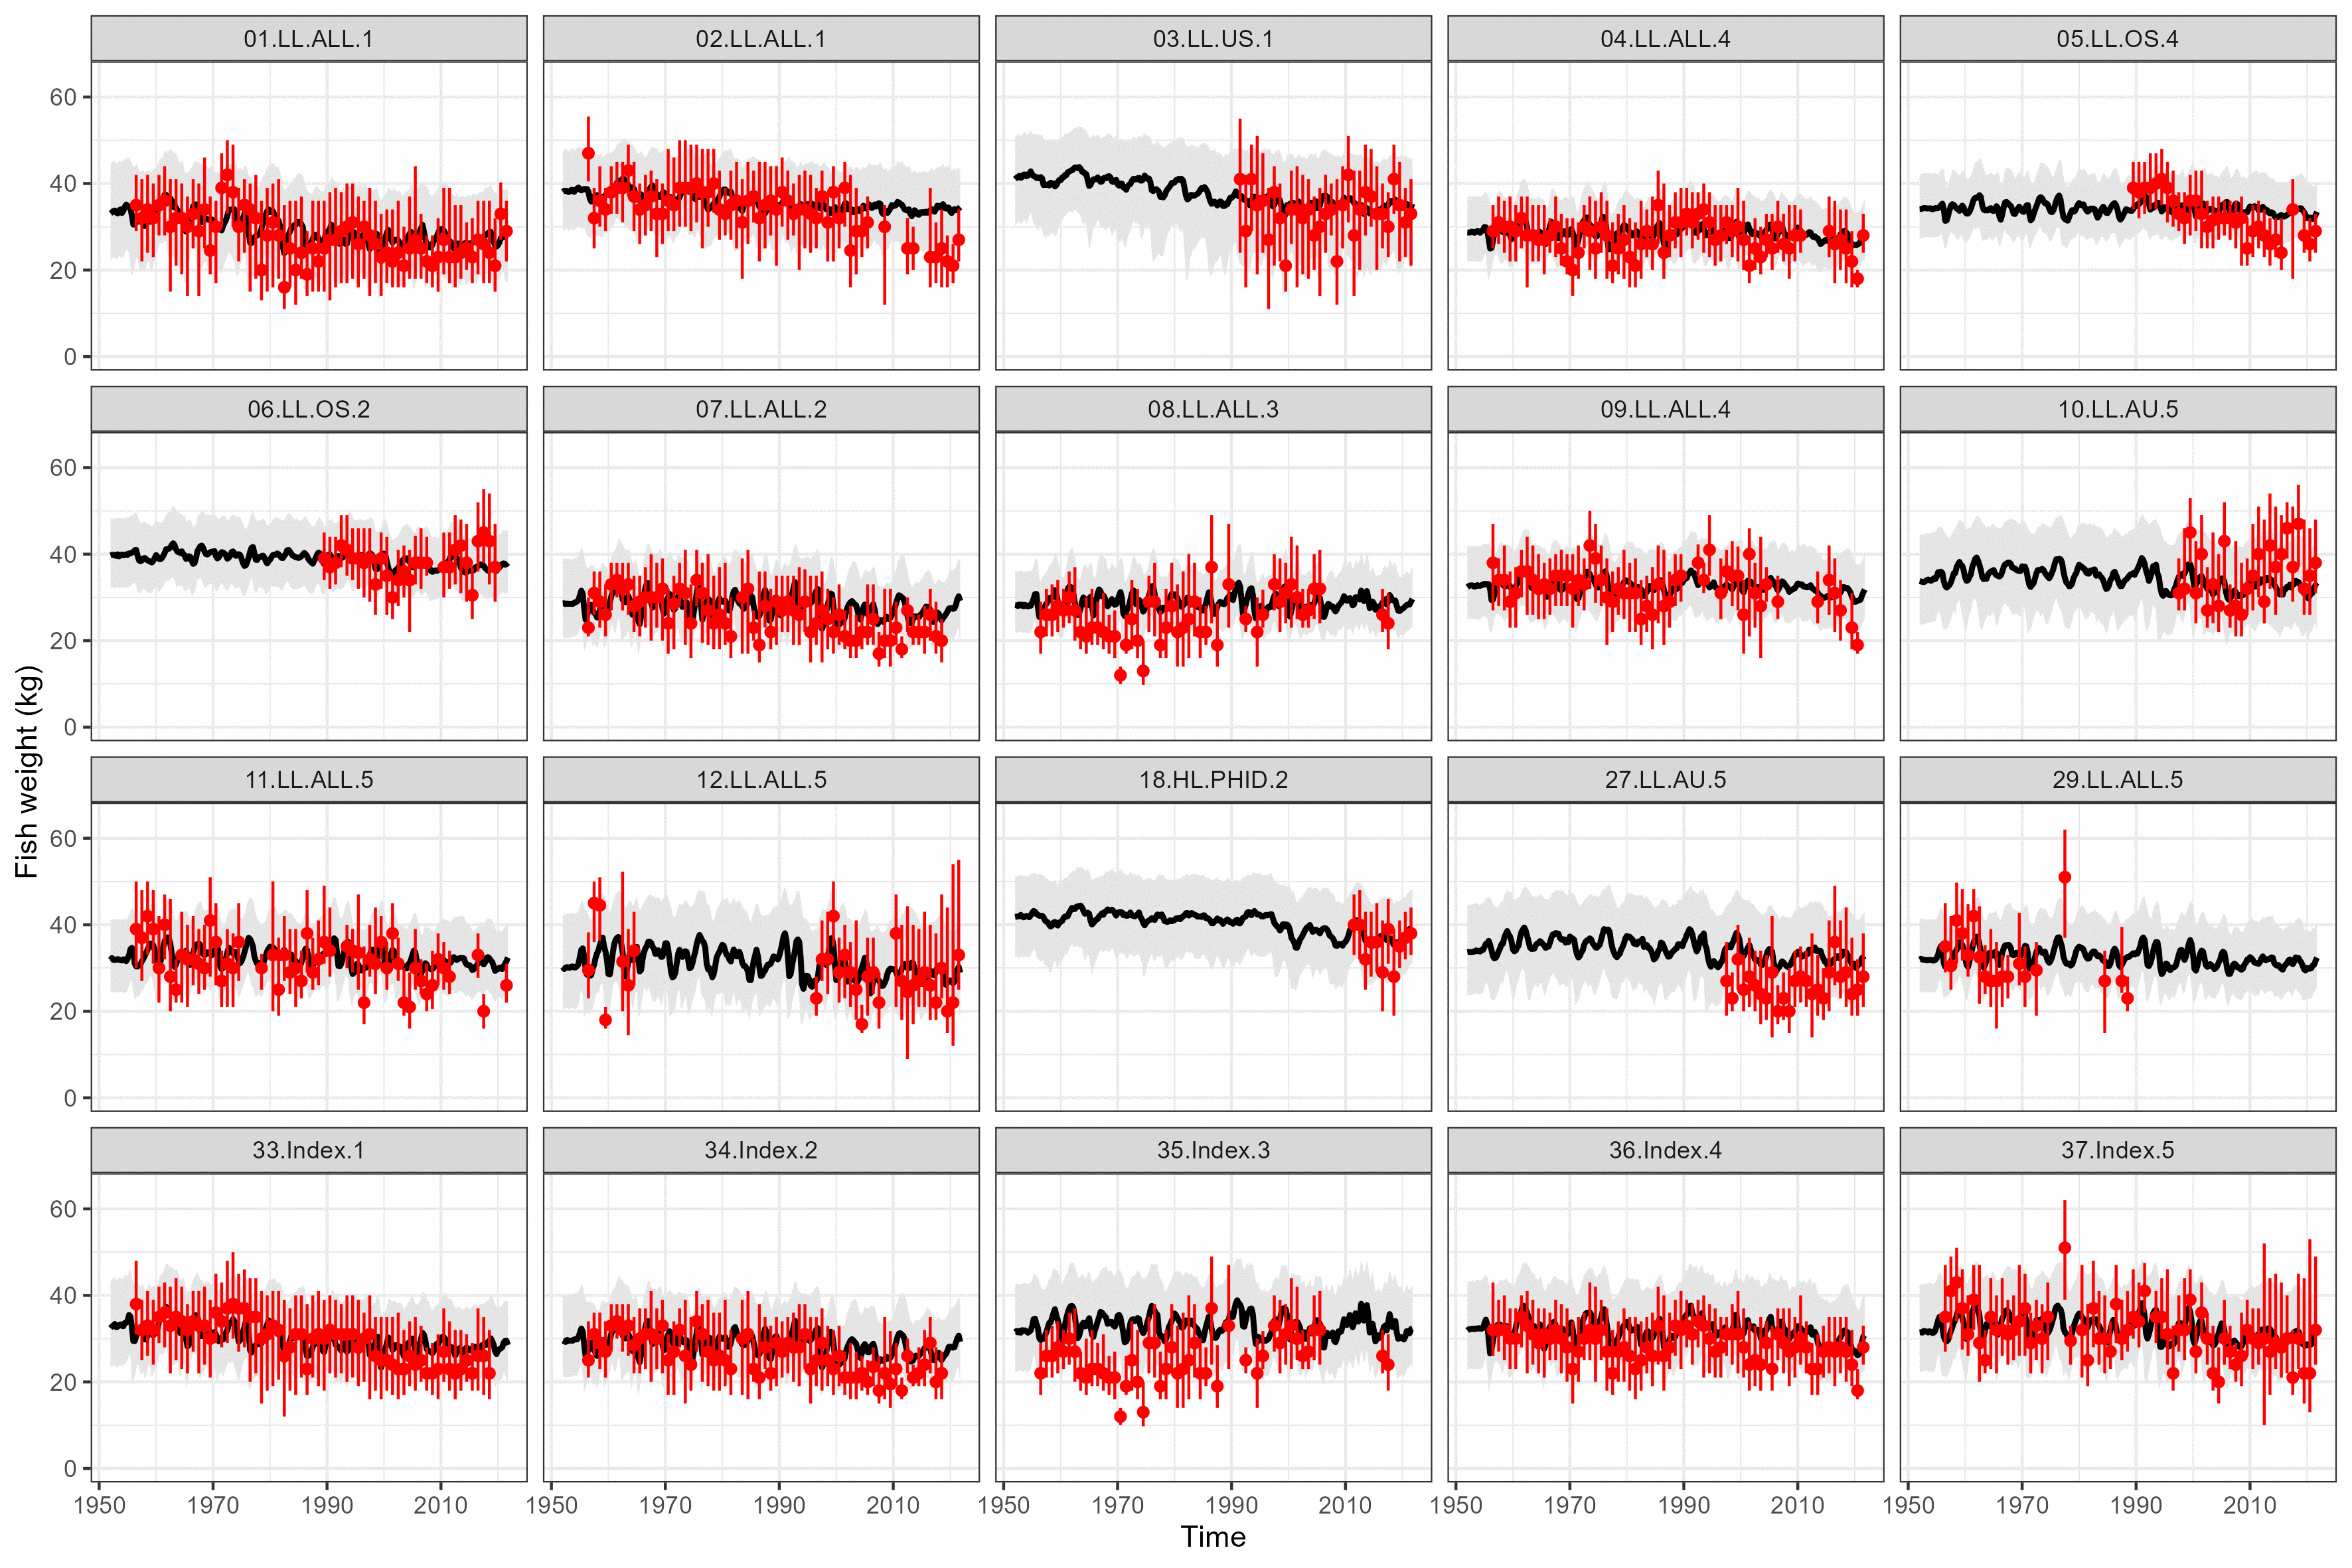
\includegraphics[width=1.3\textwidth]{weight_fit_timeseries.png}
    \caption{A comparison of the observed (red points) and predicted (black line) median fish weights (kg) for the longline fisheries in diagnostic model. The uncertainty intervals (gray shading) represent the values encompassed by the 25\% and 75\% quantiles. Sampling data are by quarter and only length samples more than 30 fish per quarter are plotted. \label{fig:weight_fit_timeseries}}
  \end{figure}
\end{landscape}
\clearpage

\newpage
\begin{figure}[!ht]
  \centering
  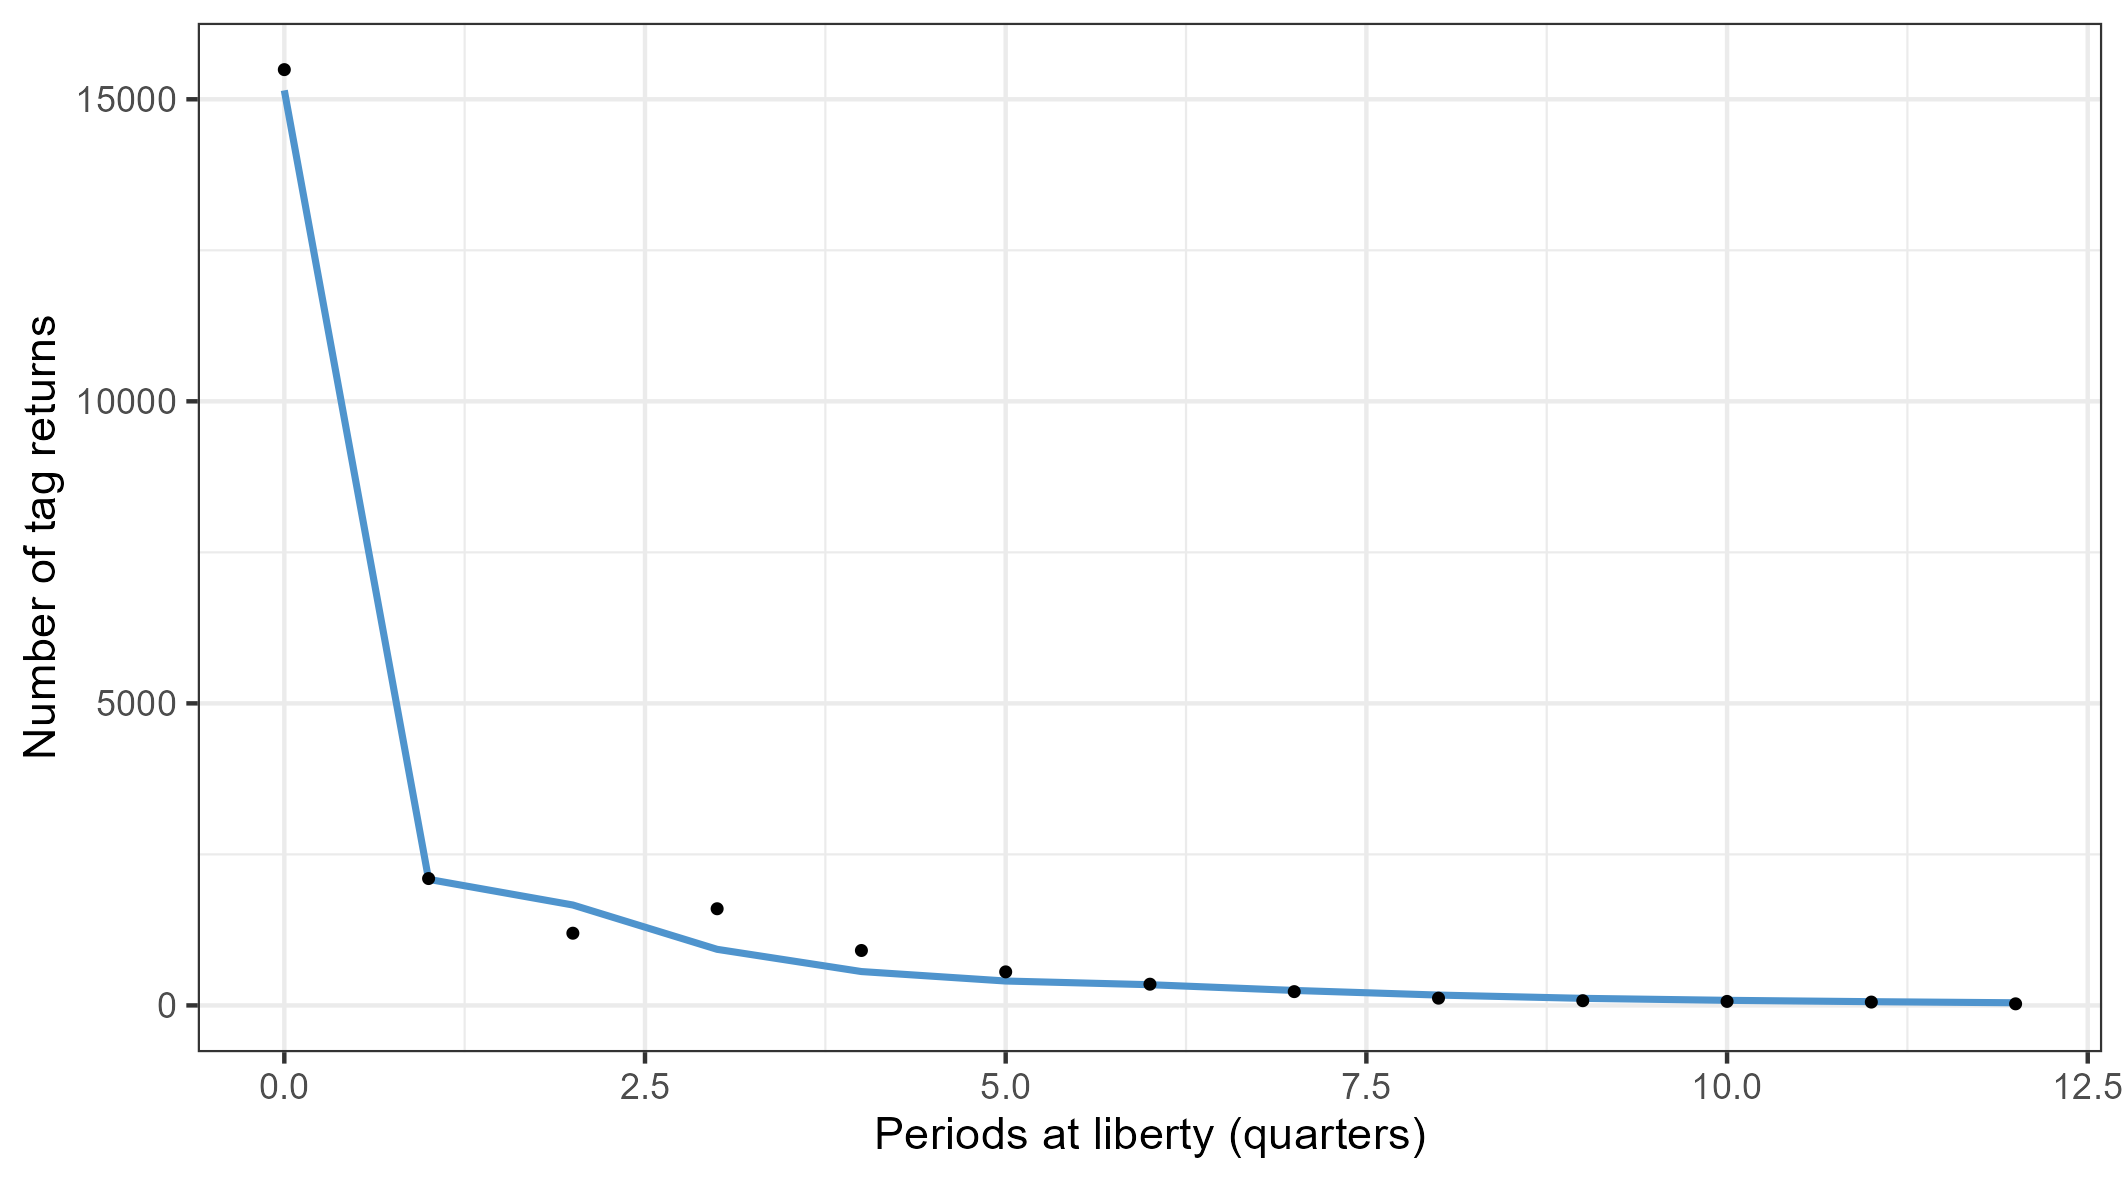
\includegraphics[width=0.9\textwidth]{tag_attrition_all.png}
  \caption{Observed (black points) and model-predicted (blue line) tag attrition across all tag release events for the diagnostic model. \label{fig:tag_attrition_all}}
\end{figure}
\clearpage

\newpage
\begin{figure}[!ht]
  \centering
  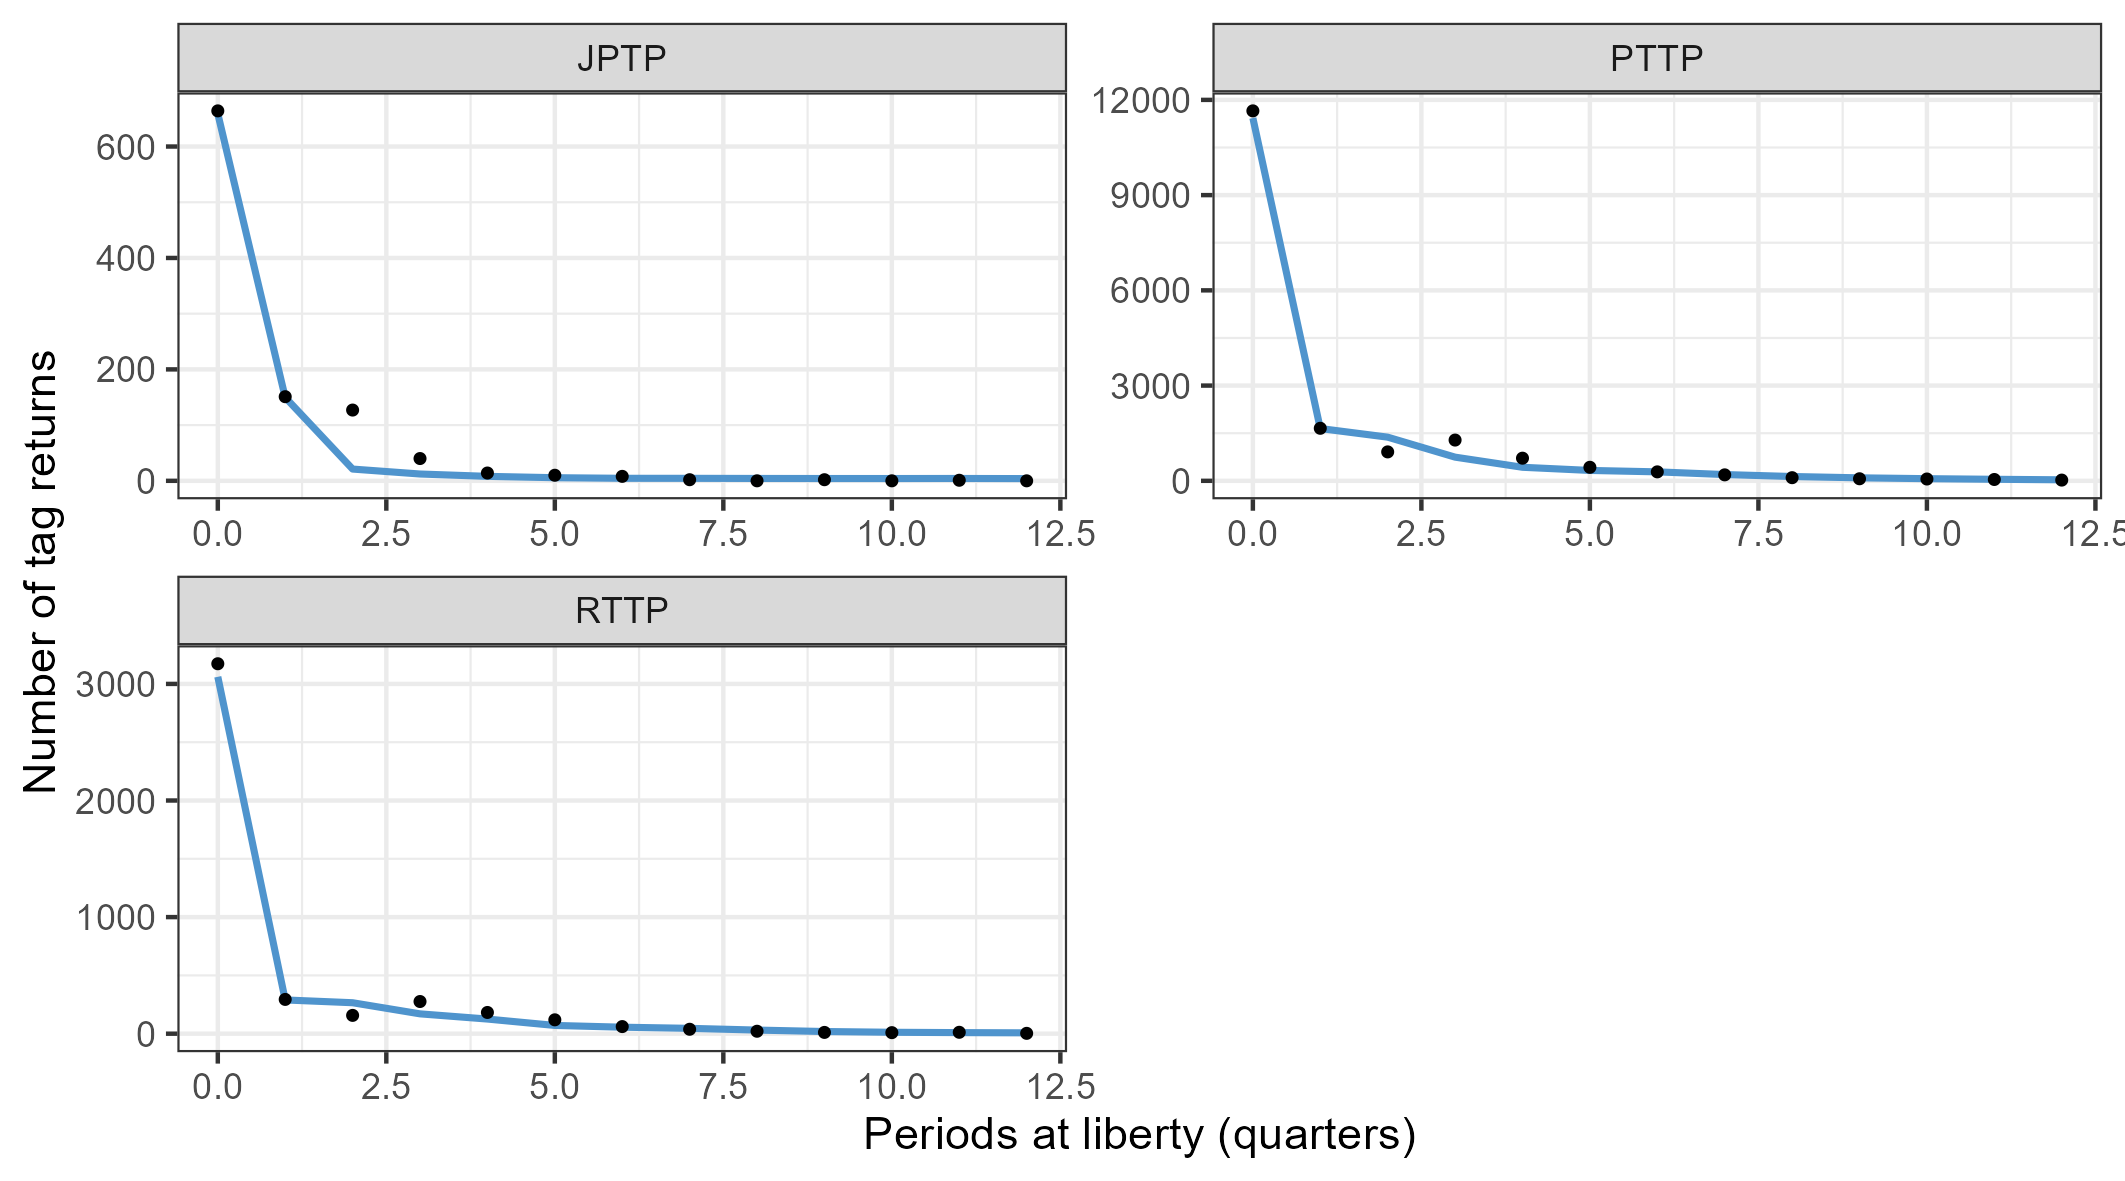
\includegraphics[width=\textwidth]{tag_attrition_by_program.png}
  \caption{Observed (black points) and model-predicted (blue line) tag attrition by tagging programme for the diagnostic model. \label{fig:tag_attrition_by_program}}
\end{figure}
\clearpage

\newpage
\begin{figure}[!ht]
  \centering
  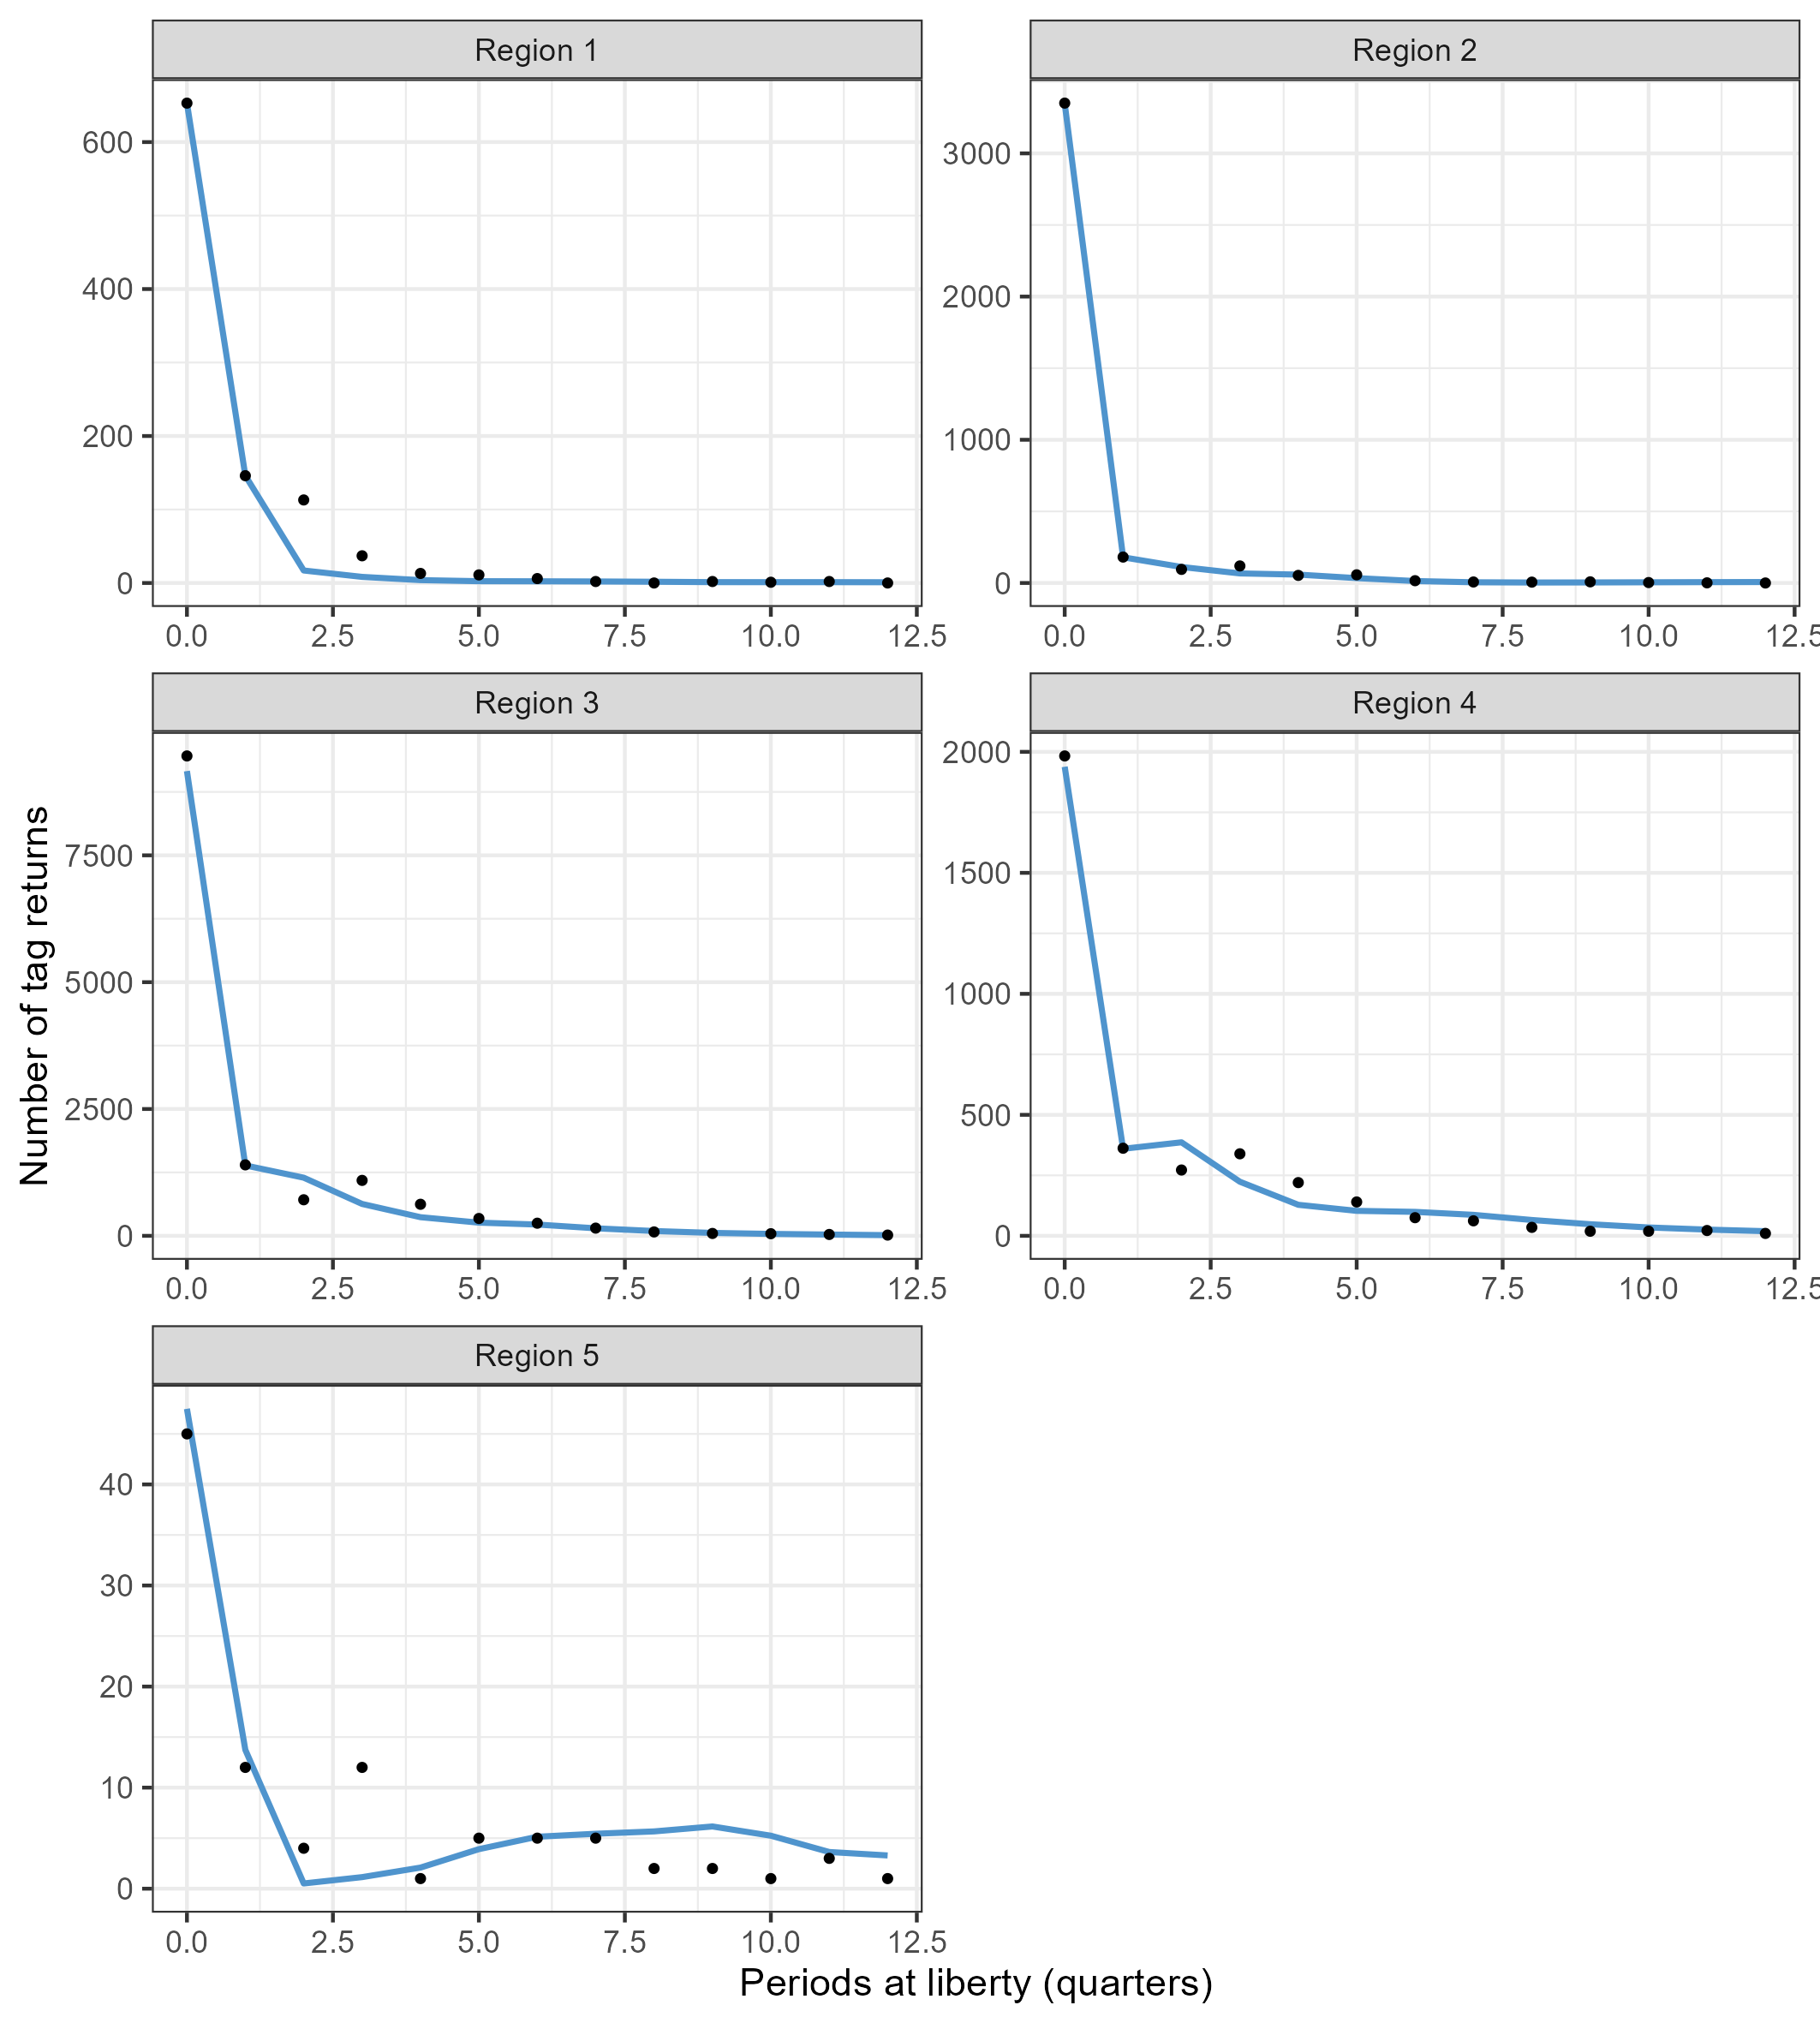
\includegraphics[width=\textwidth]{tag_attrition_by_region.png}
  \caption{Observed (black points) and model-predicted (blue line) tag attrition by region for the diagnostic model. \label{fig:tag_attrition_by_region}}
\end{figure}
\clearpage

\newpage
\begin{figure}[!ht]
  \centering
  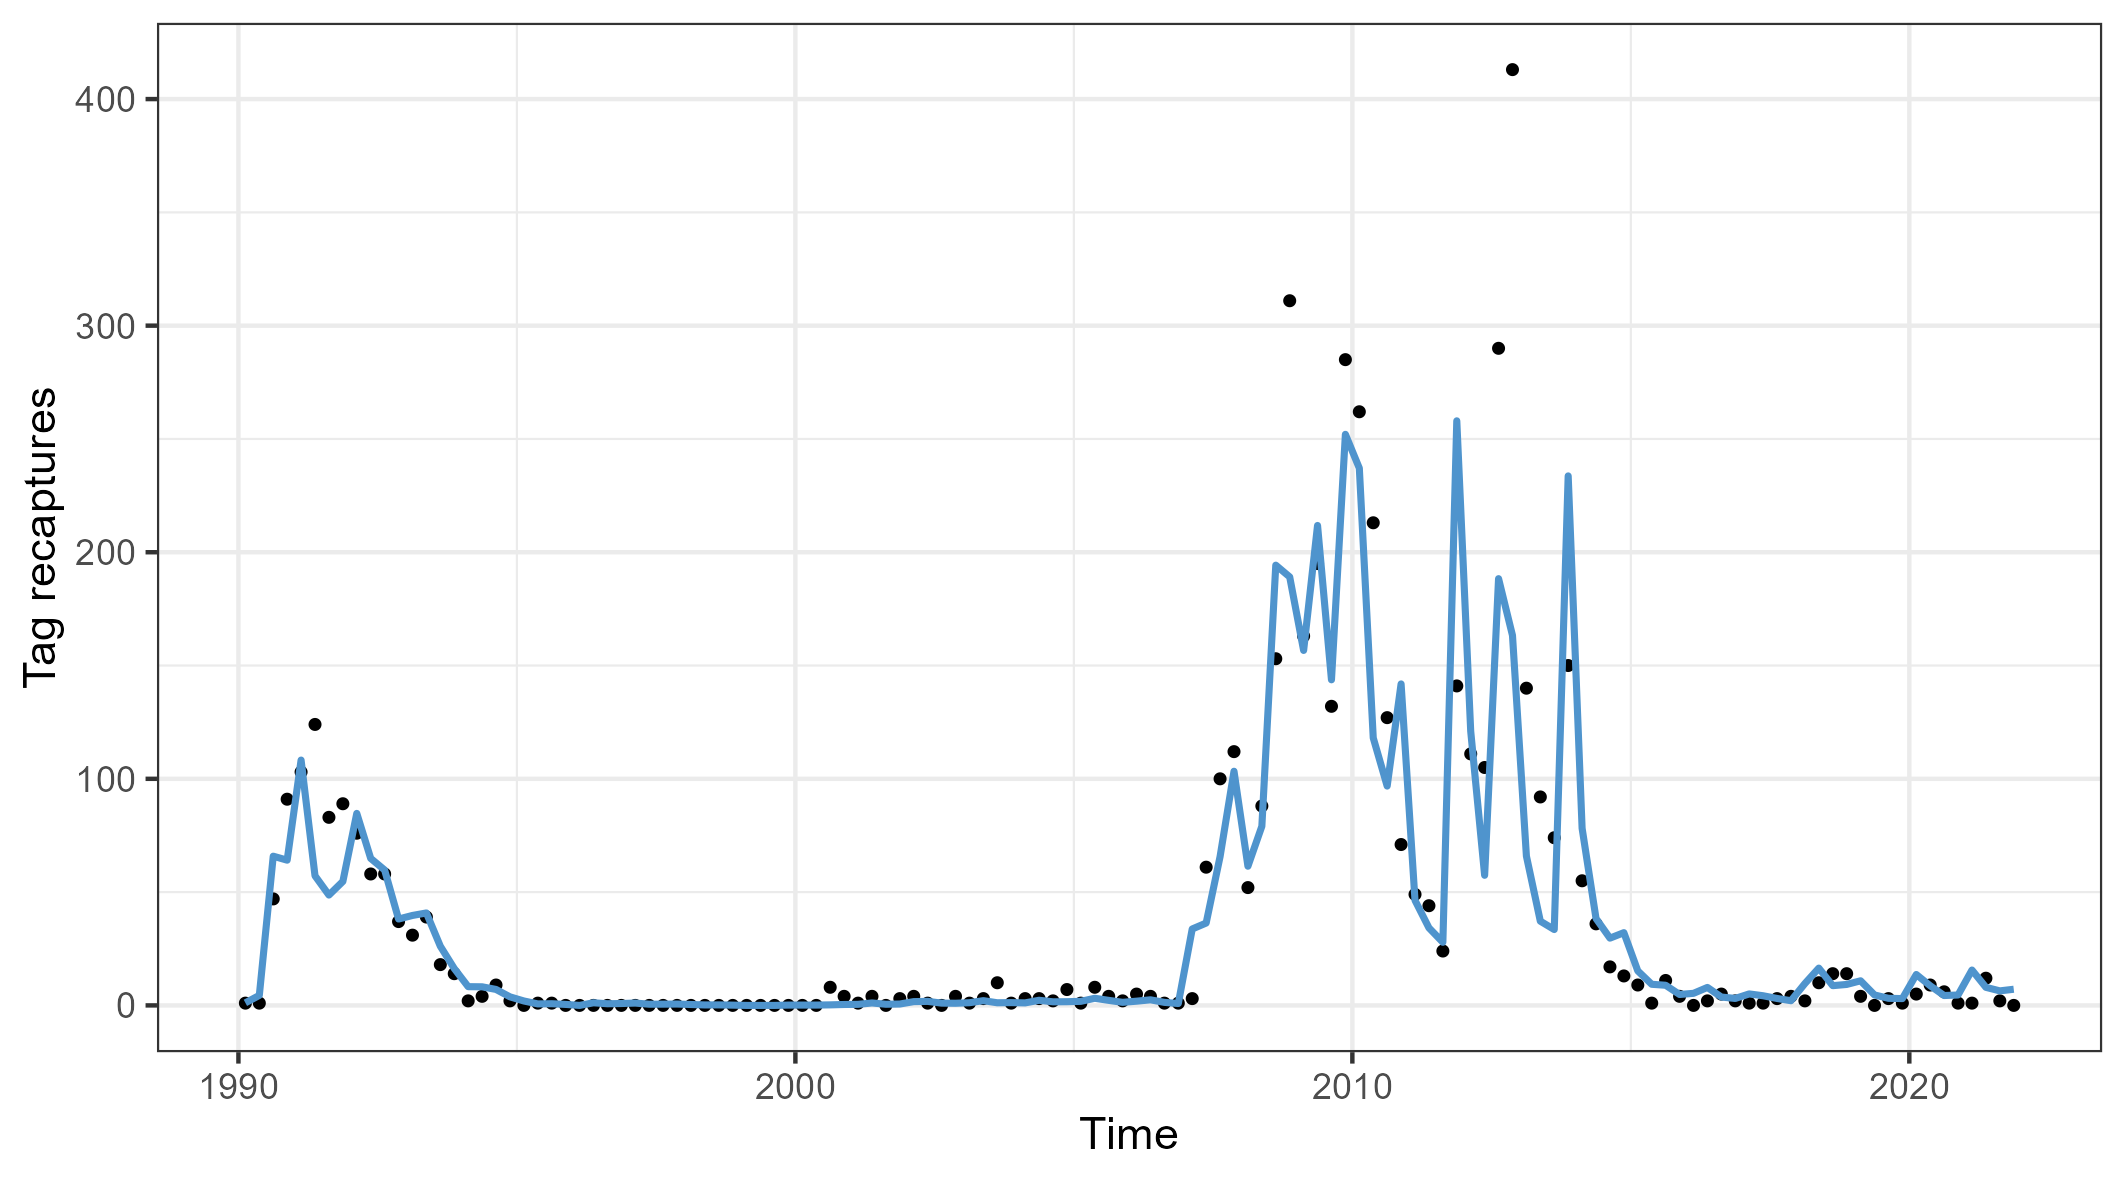
\includegraphics[width=\textwidth]{tag_returns_all.png}
  \caption{Observed (black points) and model-predicted (blue line) tag returns over time, with returns in the mixing period removed, for the diagnostic model across all tag release events with all tag recapture groupings aggregated. \label{fig:tag_returns_all_year}}
\end{figure}
\clearpage

\newpage
\begin{figure}[!ht]
  \centering
  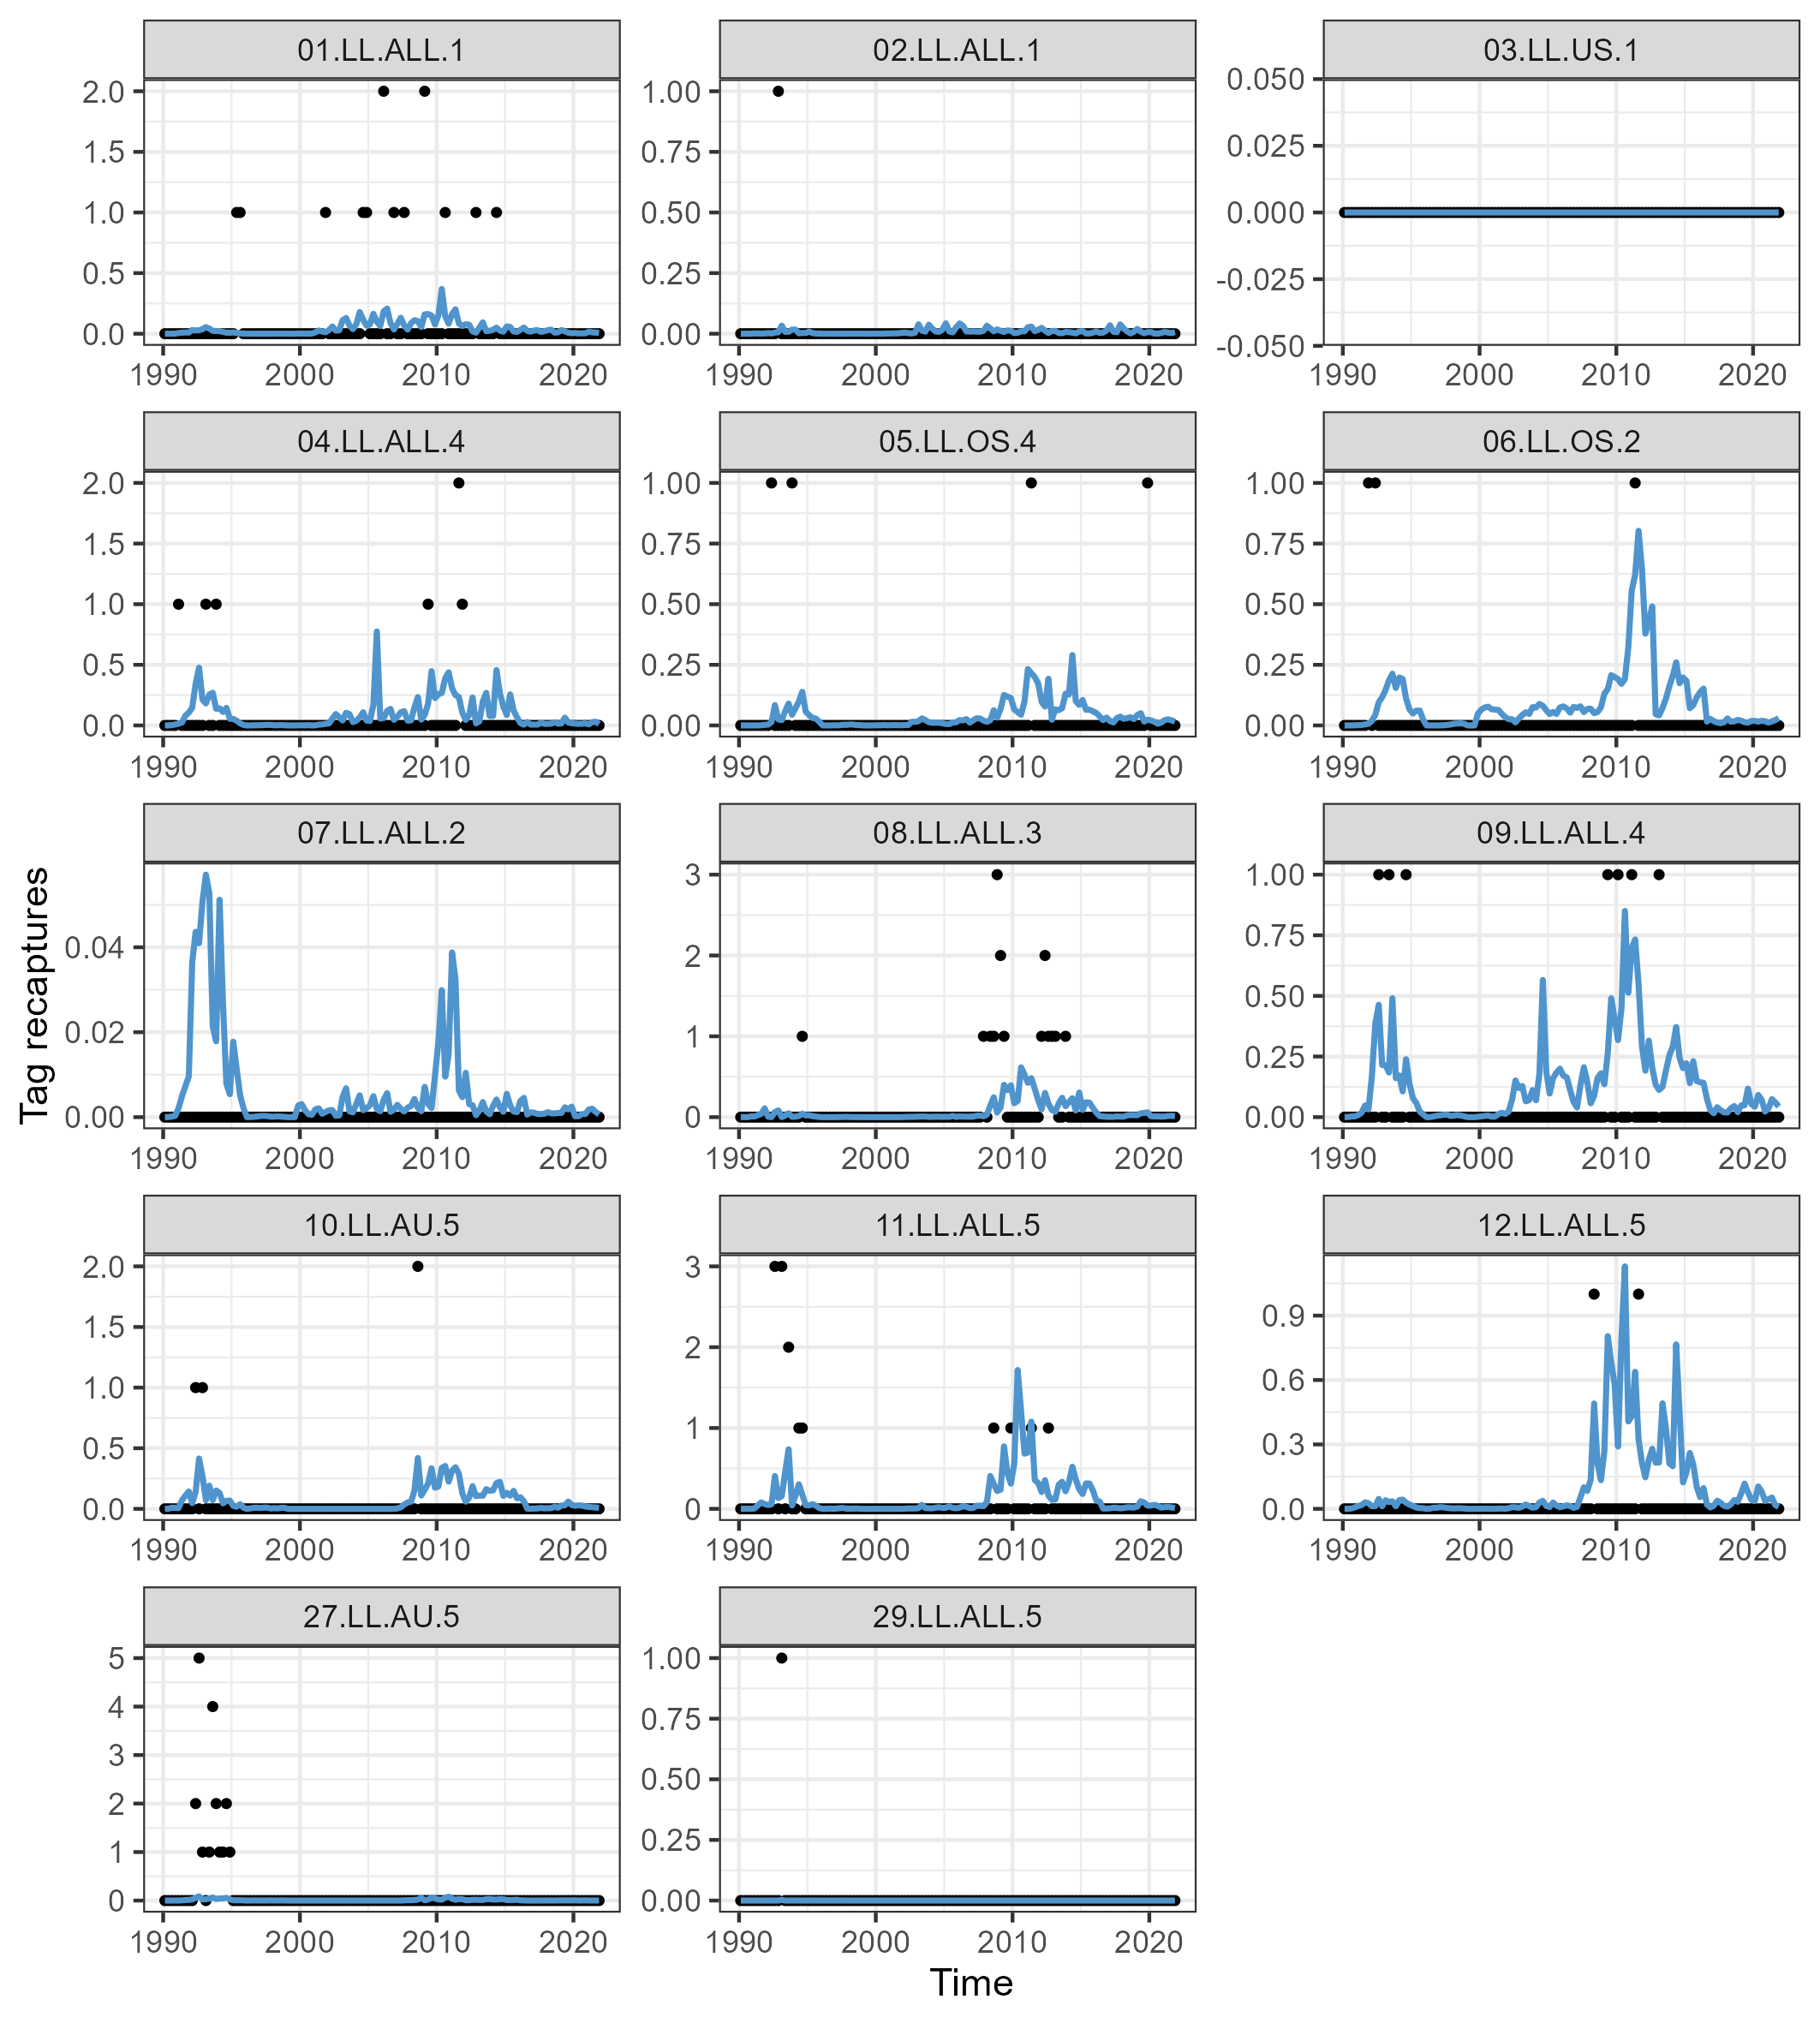
\includegraphics[width=\textwidth]{tag_returns_ll.png}
  \caption{Observed (black points) and model-predicted (blue line) tag returns over time, with returns in the mixing period removed, for the diagnostic model for longline fisheries. \label{fig:tag_returns_by_fishery_ll}}
\end{figure}
\clearpage

\newpage
\begin{figure}[!ht]
  \centering
  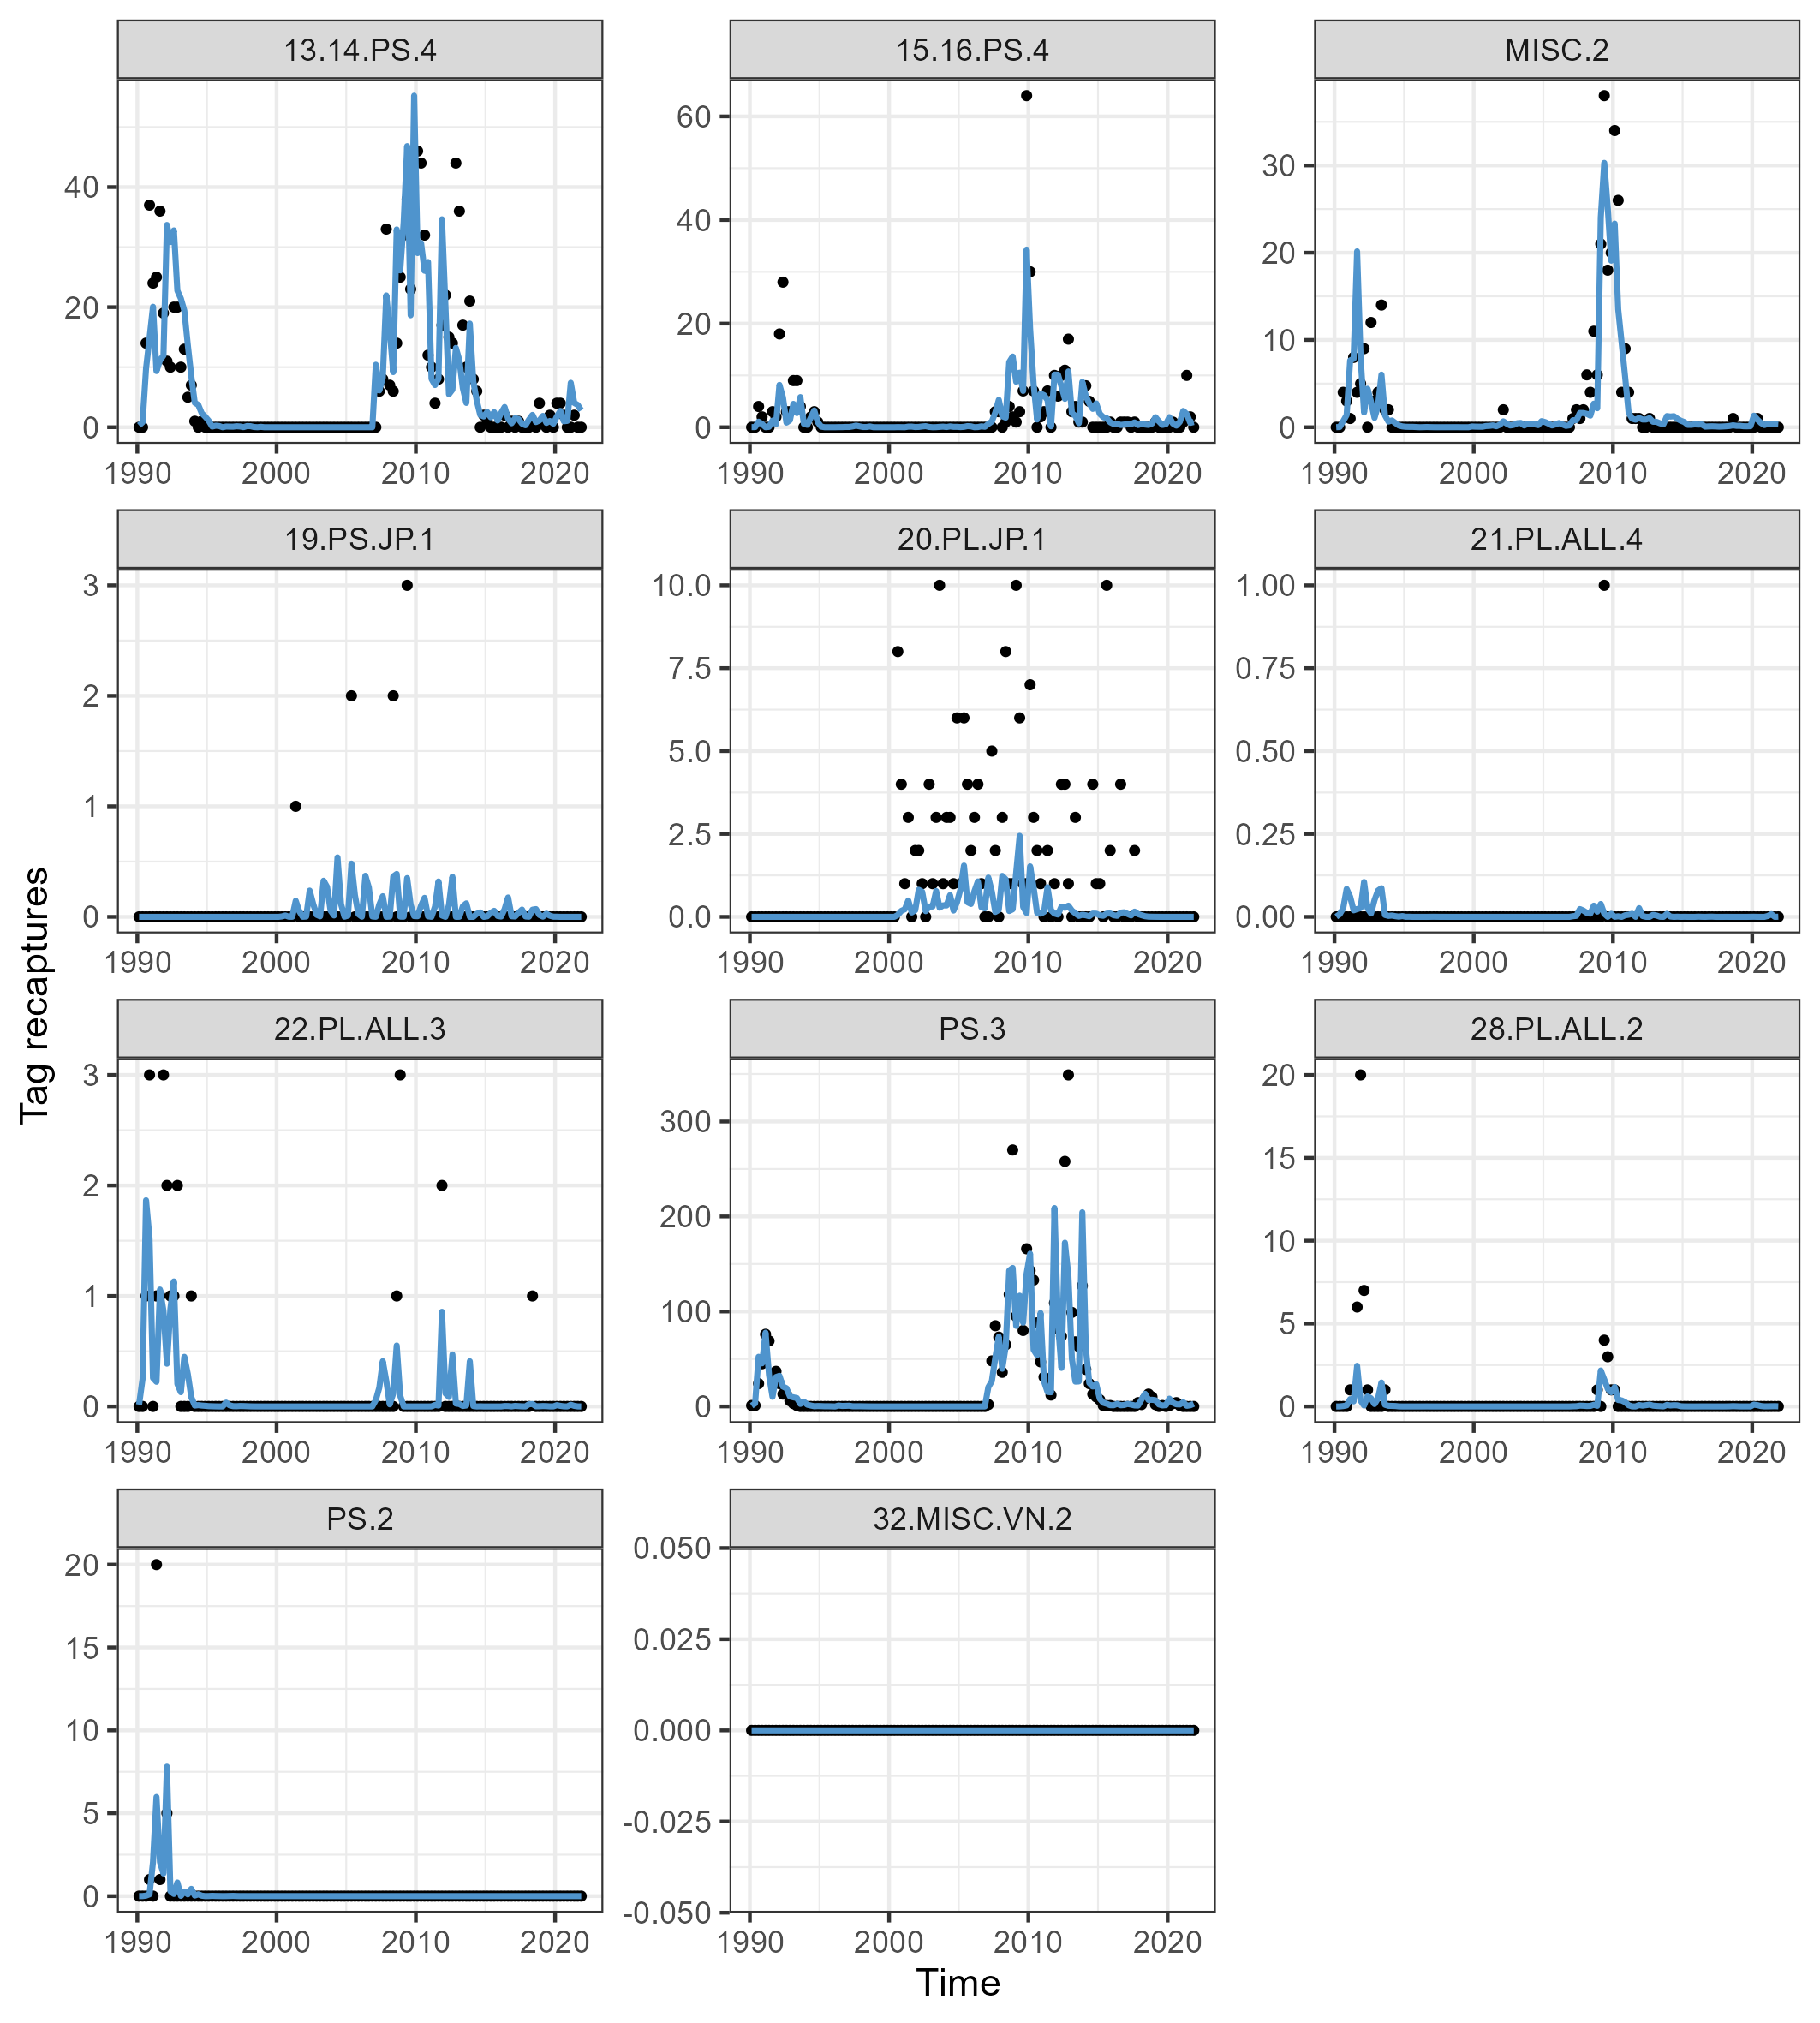
\includegraphics[width=\textwidth]{tag_returns_oth.png}
  \caption{Observed (black points) and model-predicted (blue line) tag returns over time, with returns in the mixing period removed, for the diagnostic model for other (non-longline) fisheries. \label{fig:tag_returns_by_fishery_oth}}
\end{figure}
\clearpage

\newpage
\begin{figure}[!ht]
  \centering
  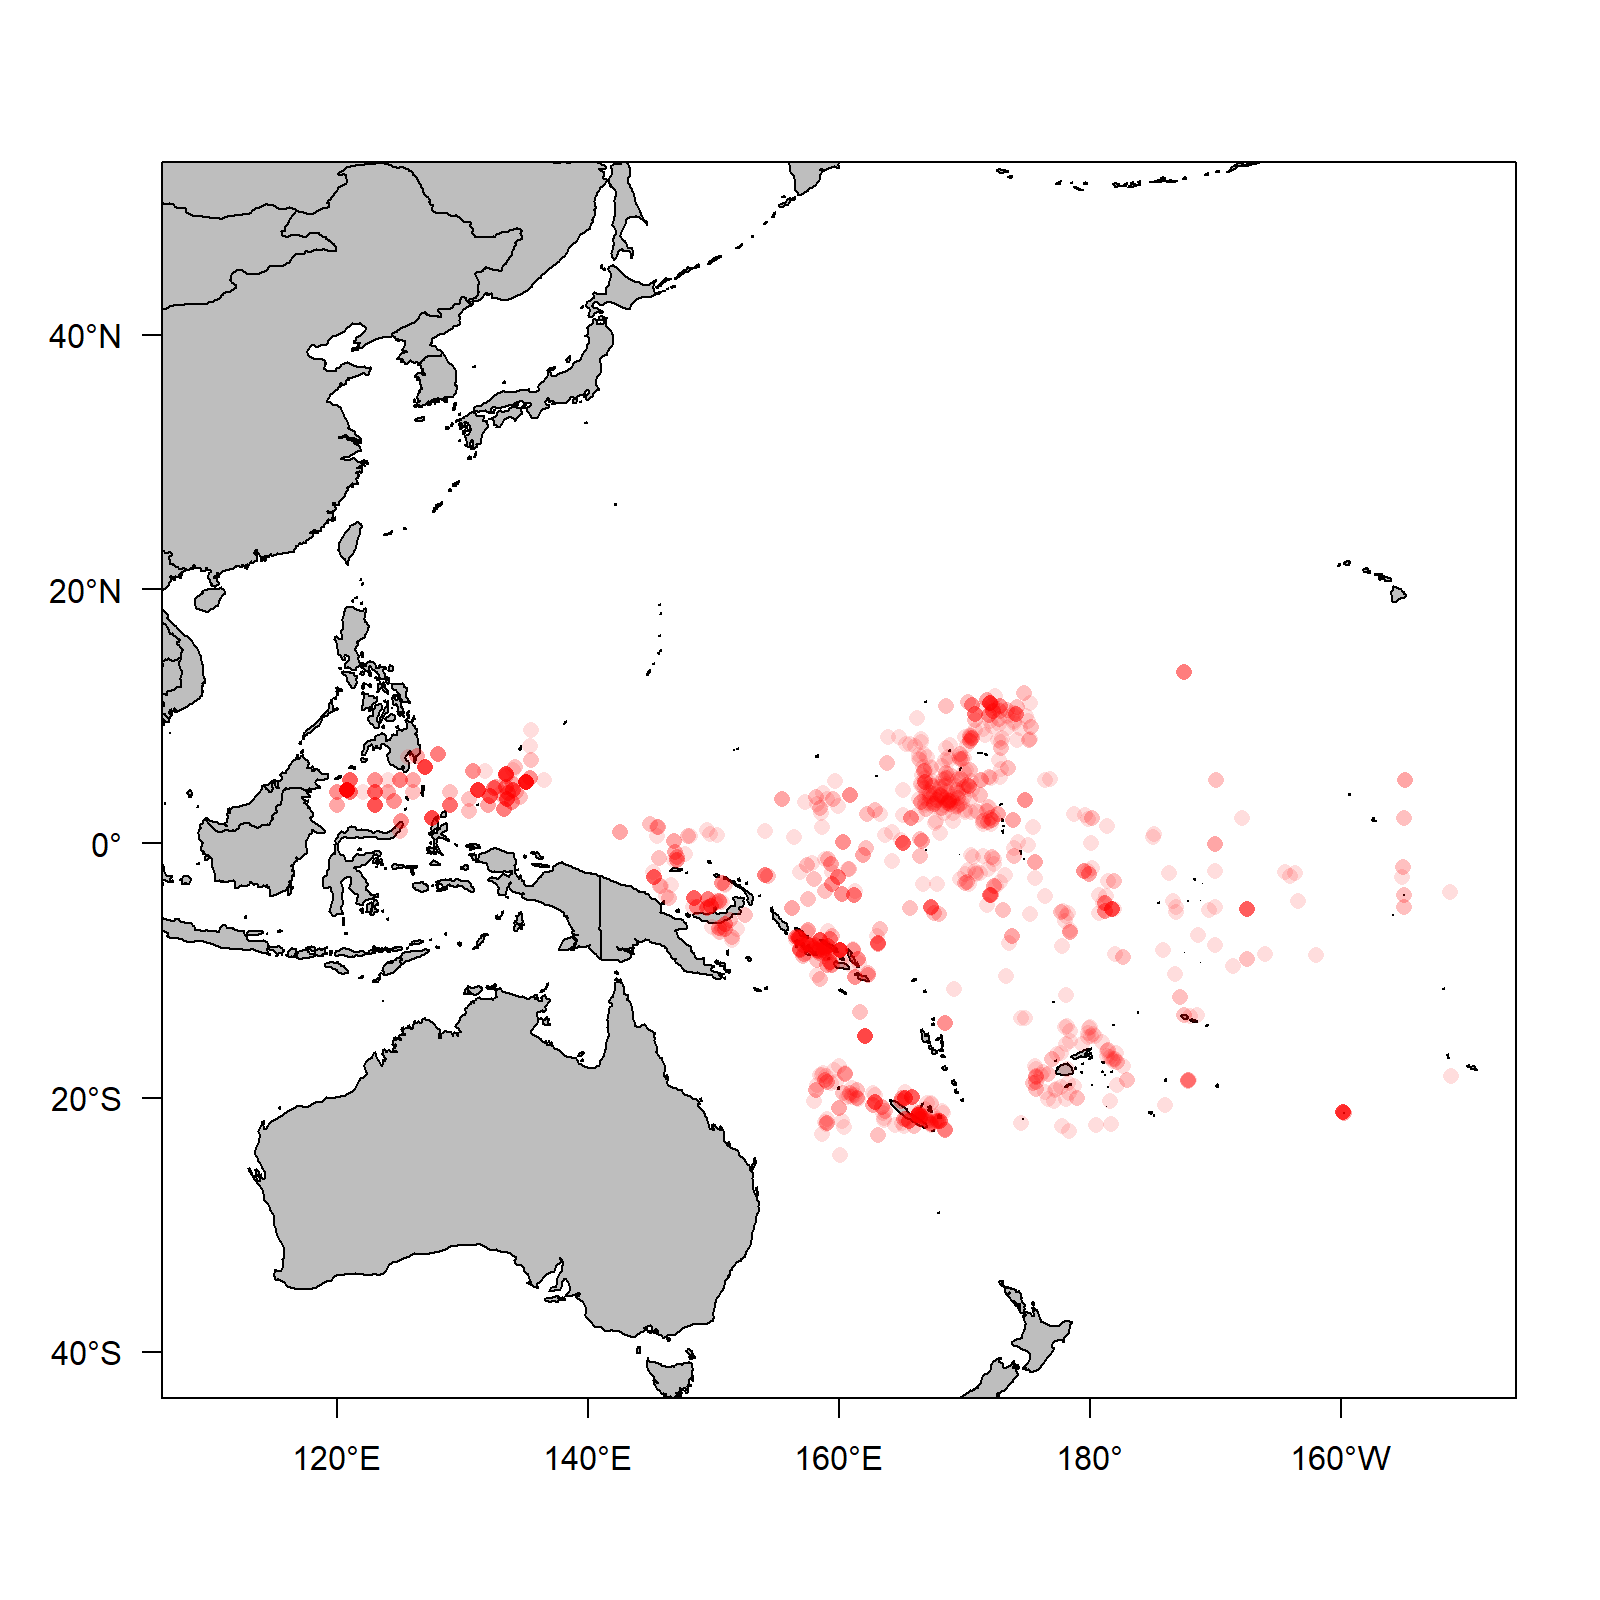
\includegraphics[width=0.9\textwidth]{otolith_map.png}
  \caption{Sample locations of otoliths $(n=1471)$ used in the assessment model to inform internal growth estimation. Single otoliths are shown as pink circles and overlapping otoliths as progressively more saturated red circles. \label{fig:otolith_map}}
\end{figure}
\clearpage

\newpage
\begin{figure}[!ht]
  \centering
  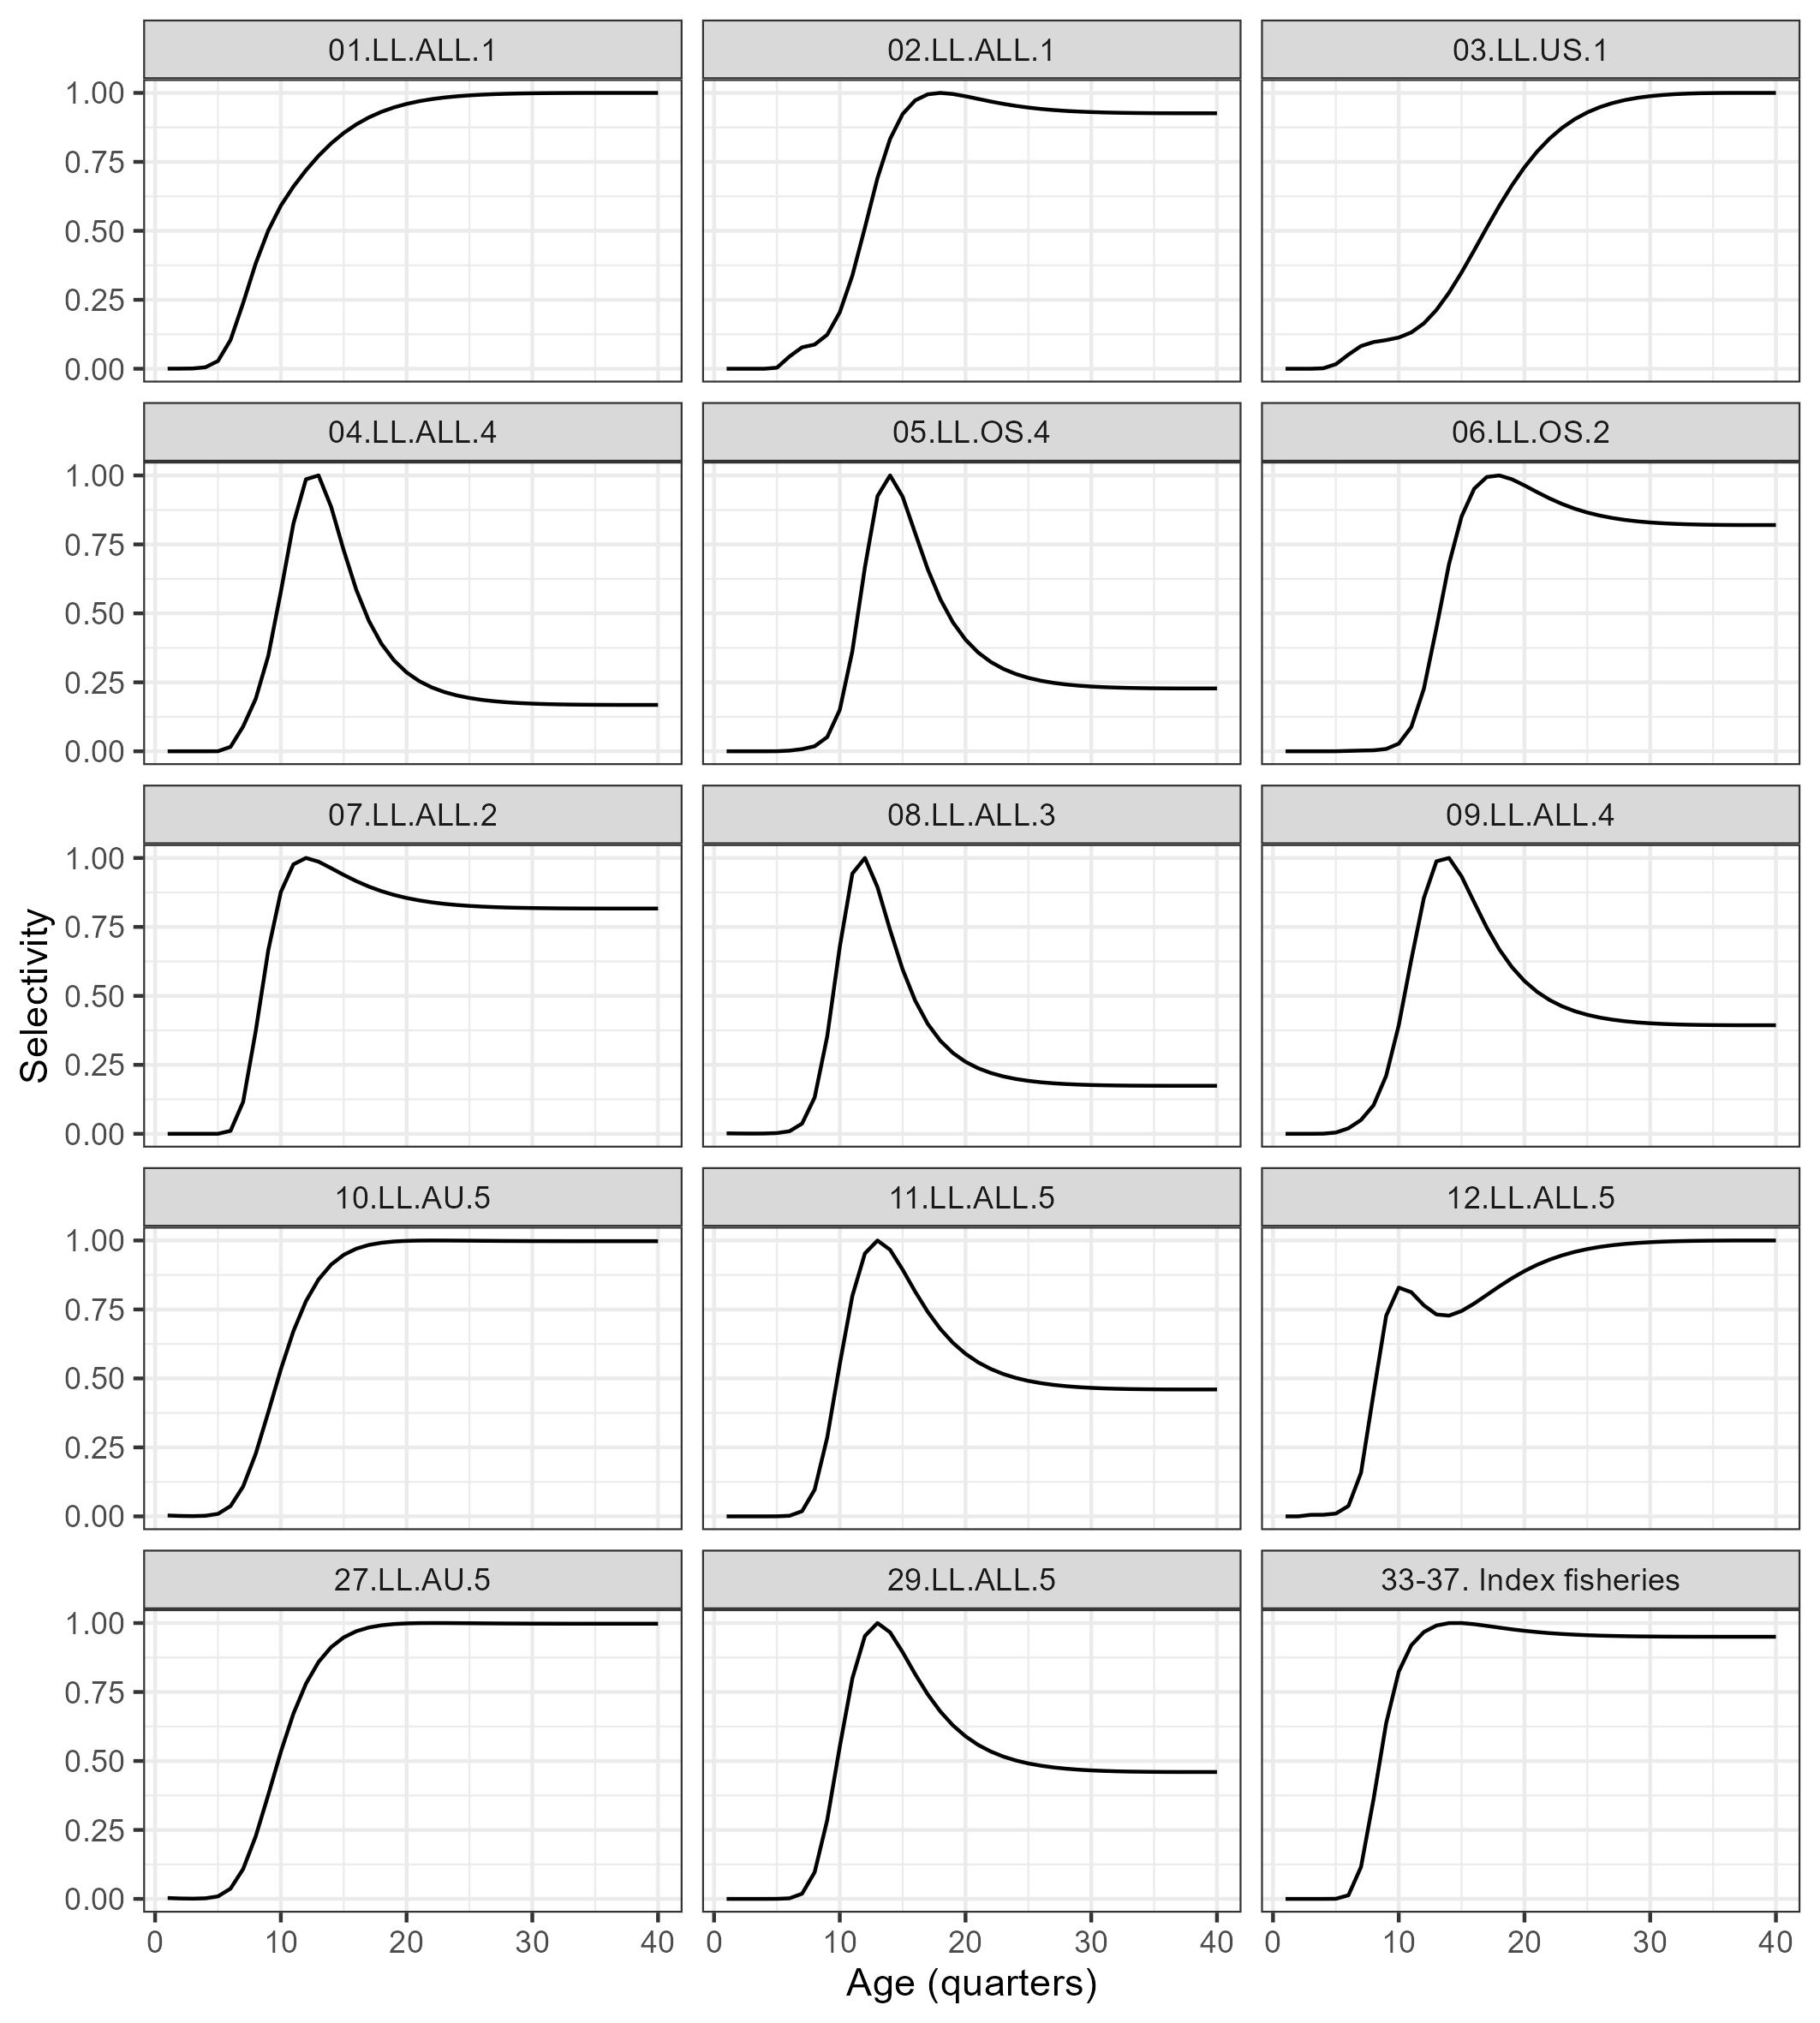
\includegraphics[width=\textwidth]{select_LL_and_index_age.png}
  \caption{Age-specific selectivity coefficients for longline fisheries with shared selectivities, with one panel for index fisheries which share selectivity across model regions. \label{fig:select_LL_and_index_age}}
\end{figure}
\clearpage

\newpage
\begin{figure}[!ht]
  \centering
  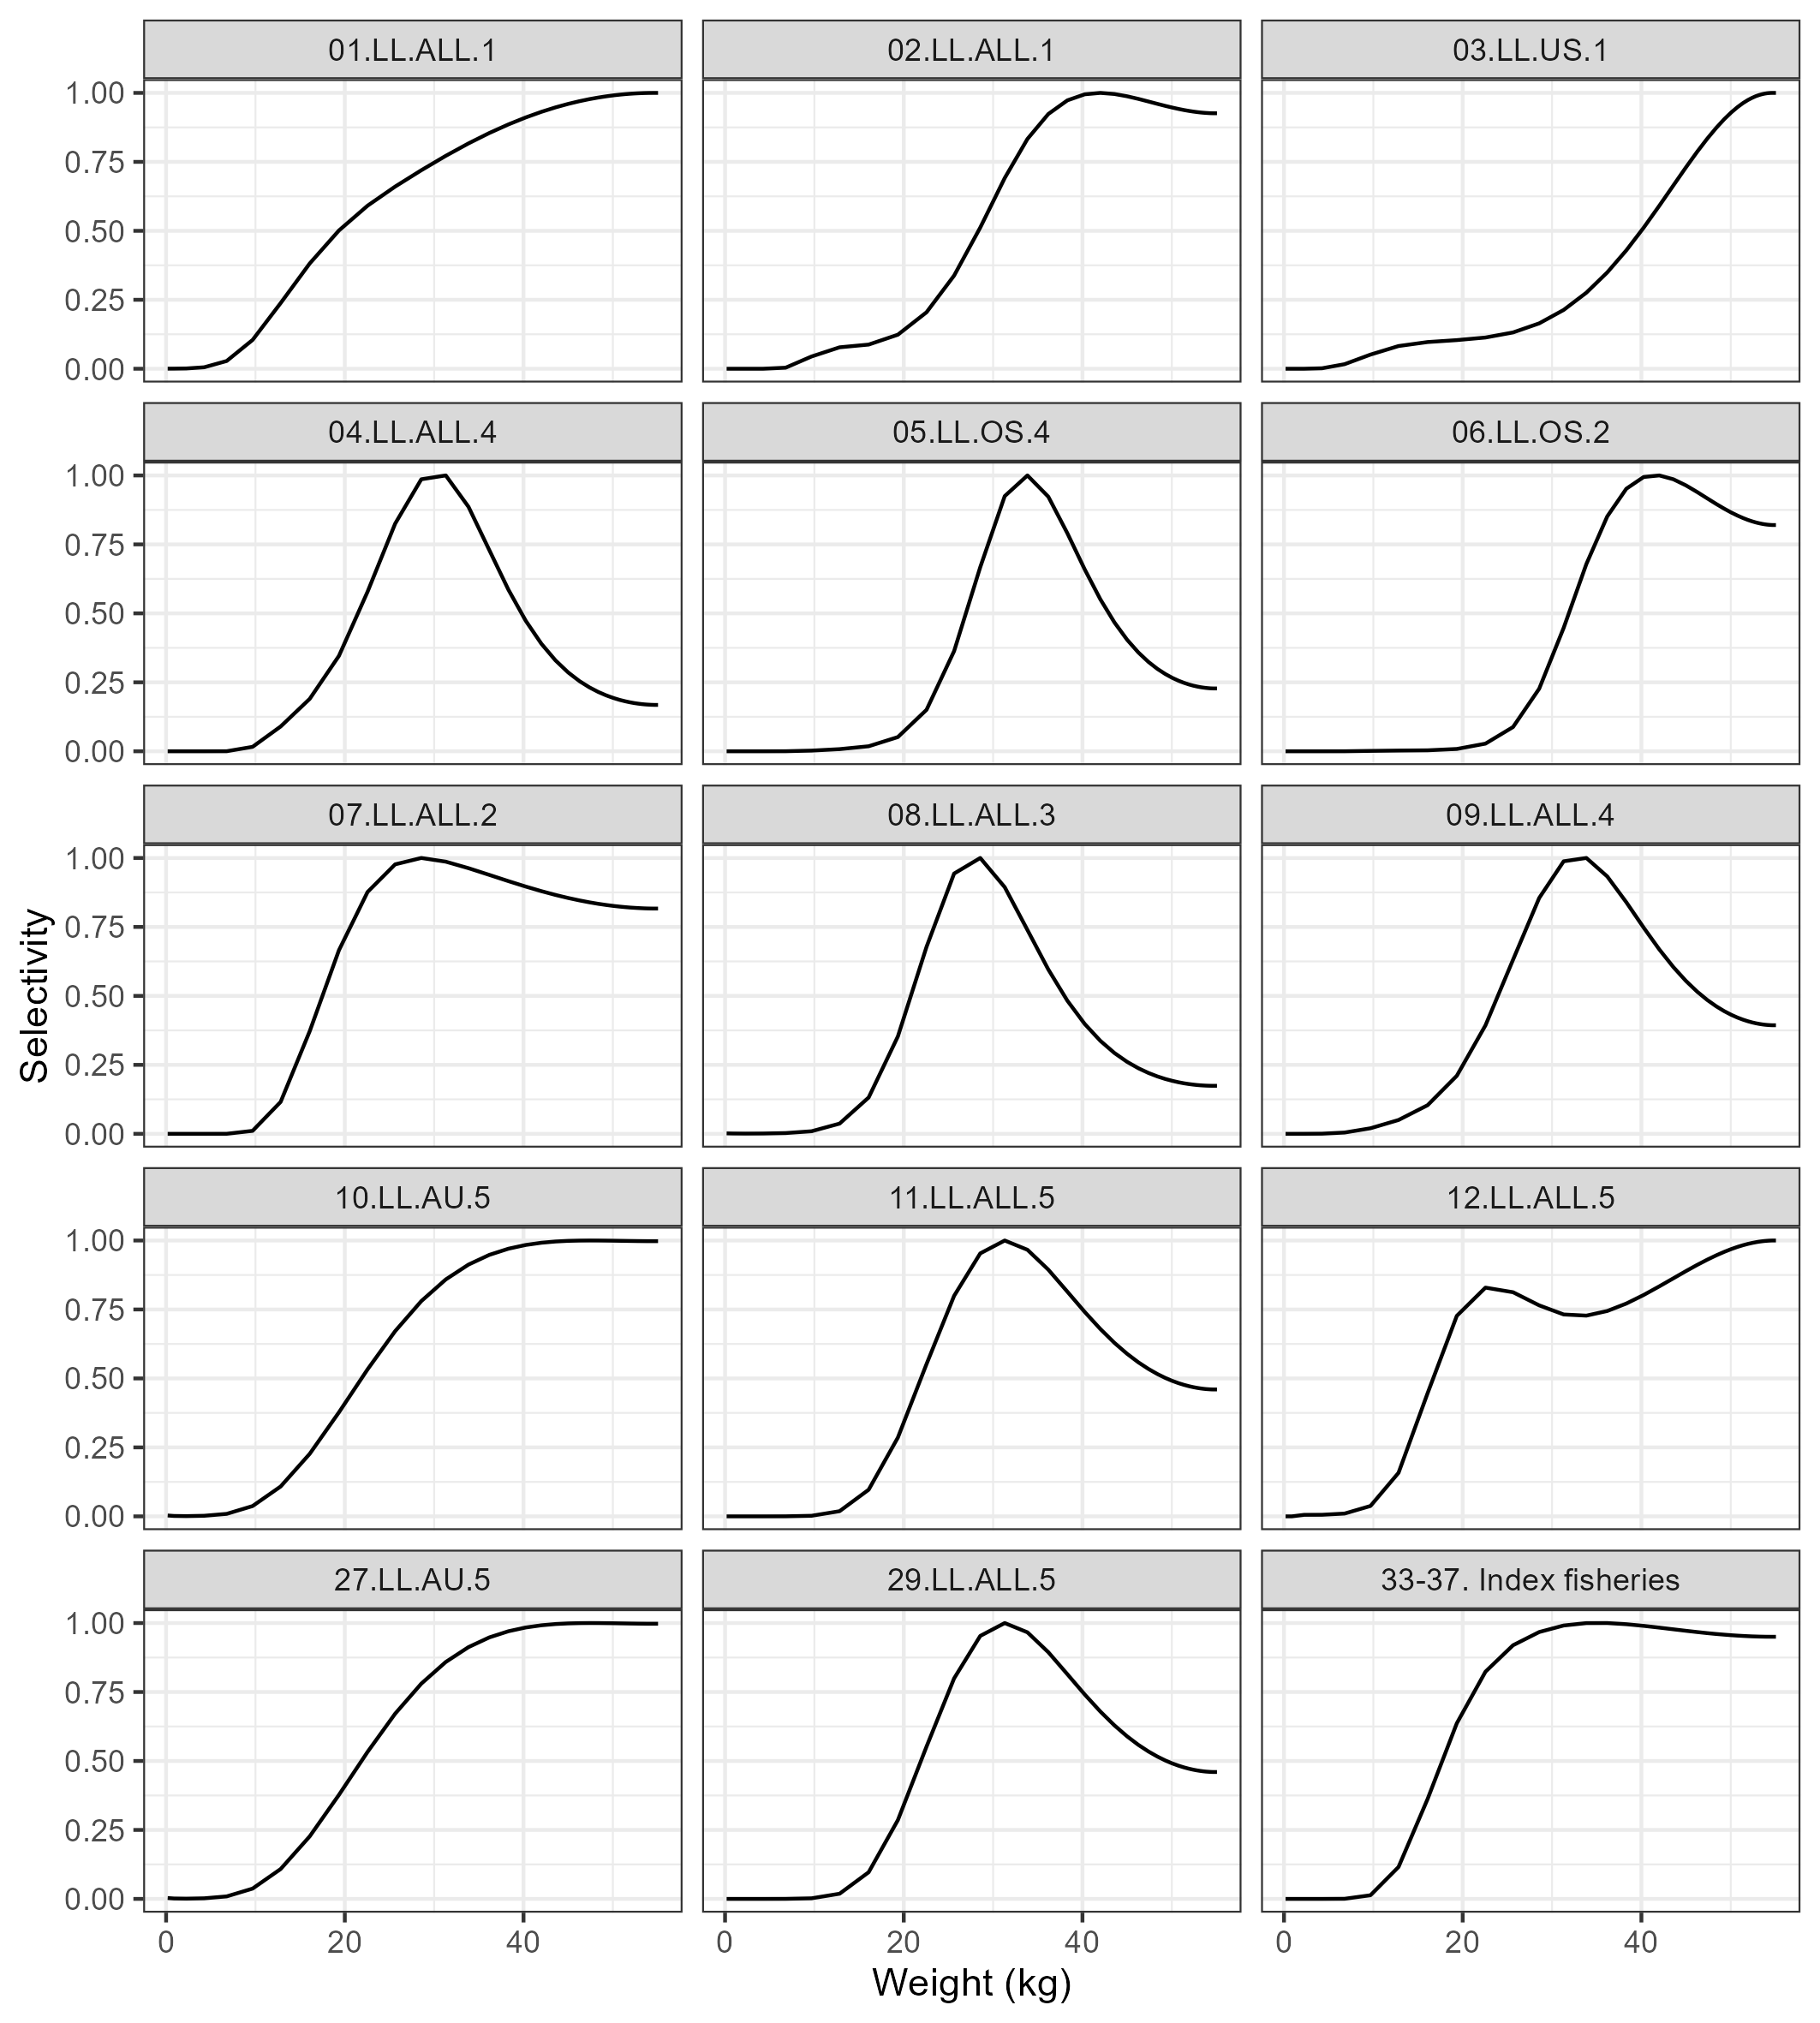
\includegraphics[width=\textwidth]{select_LL_and_index_wt.png}
  \caption{Weight-specific selectivity coefficients for longline fisheries with shared selectivities, with one panel for index fisheries which share selectivity across model regions. \label{fig:select_LL_and_index_wt}}
\end{figure}
\clearpage

\newpage
\begin{figure}[!ht]
  \centering
  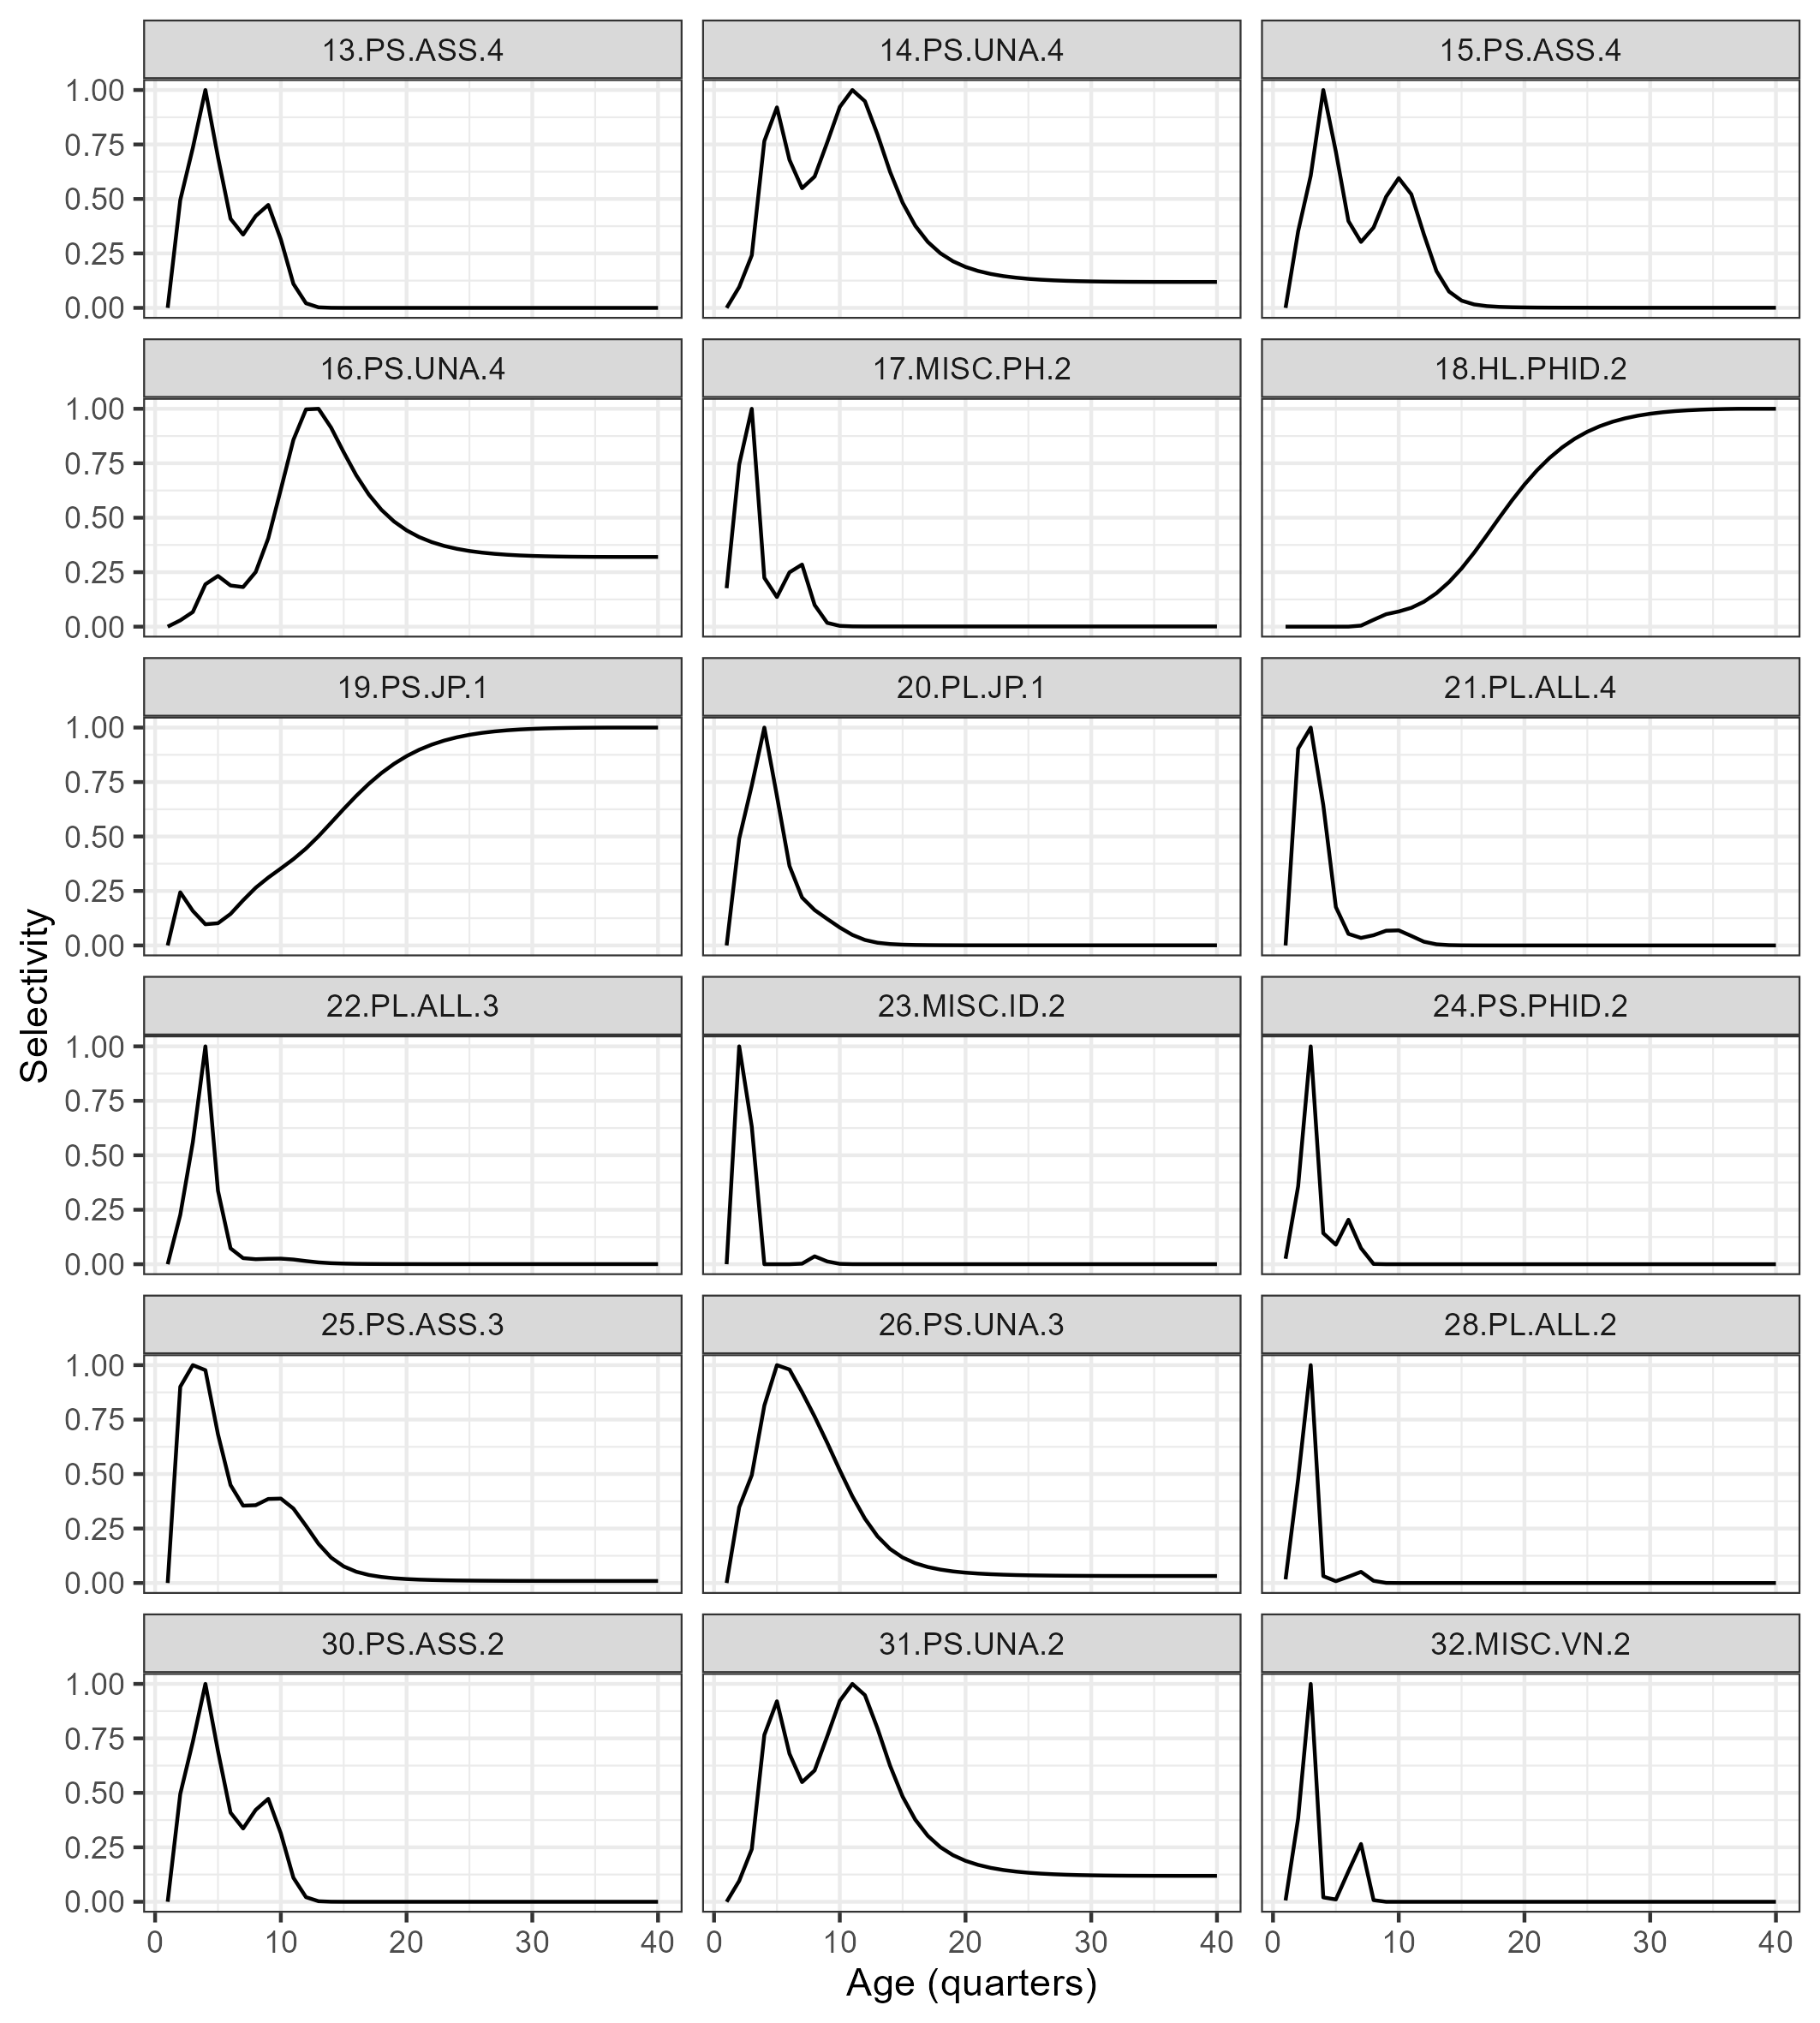
\includegraphics[width=\textwidth]{select_other_age.png}
  \caption{Age-specific selectivity coefficients by groups of fisheries with shared selectivities for miscellaneous and pole and line fisheries. \label{fig:select_other_age}}
\end{figure}
\clearpage

\newpage
\begin{figure}[!ht]
  \centering
  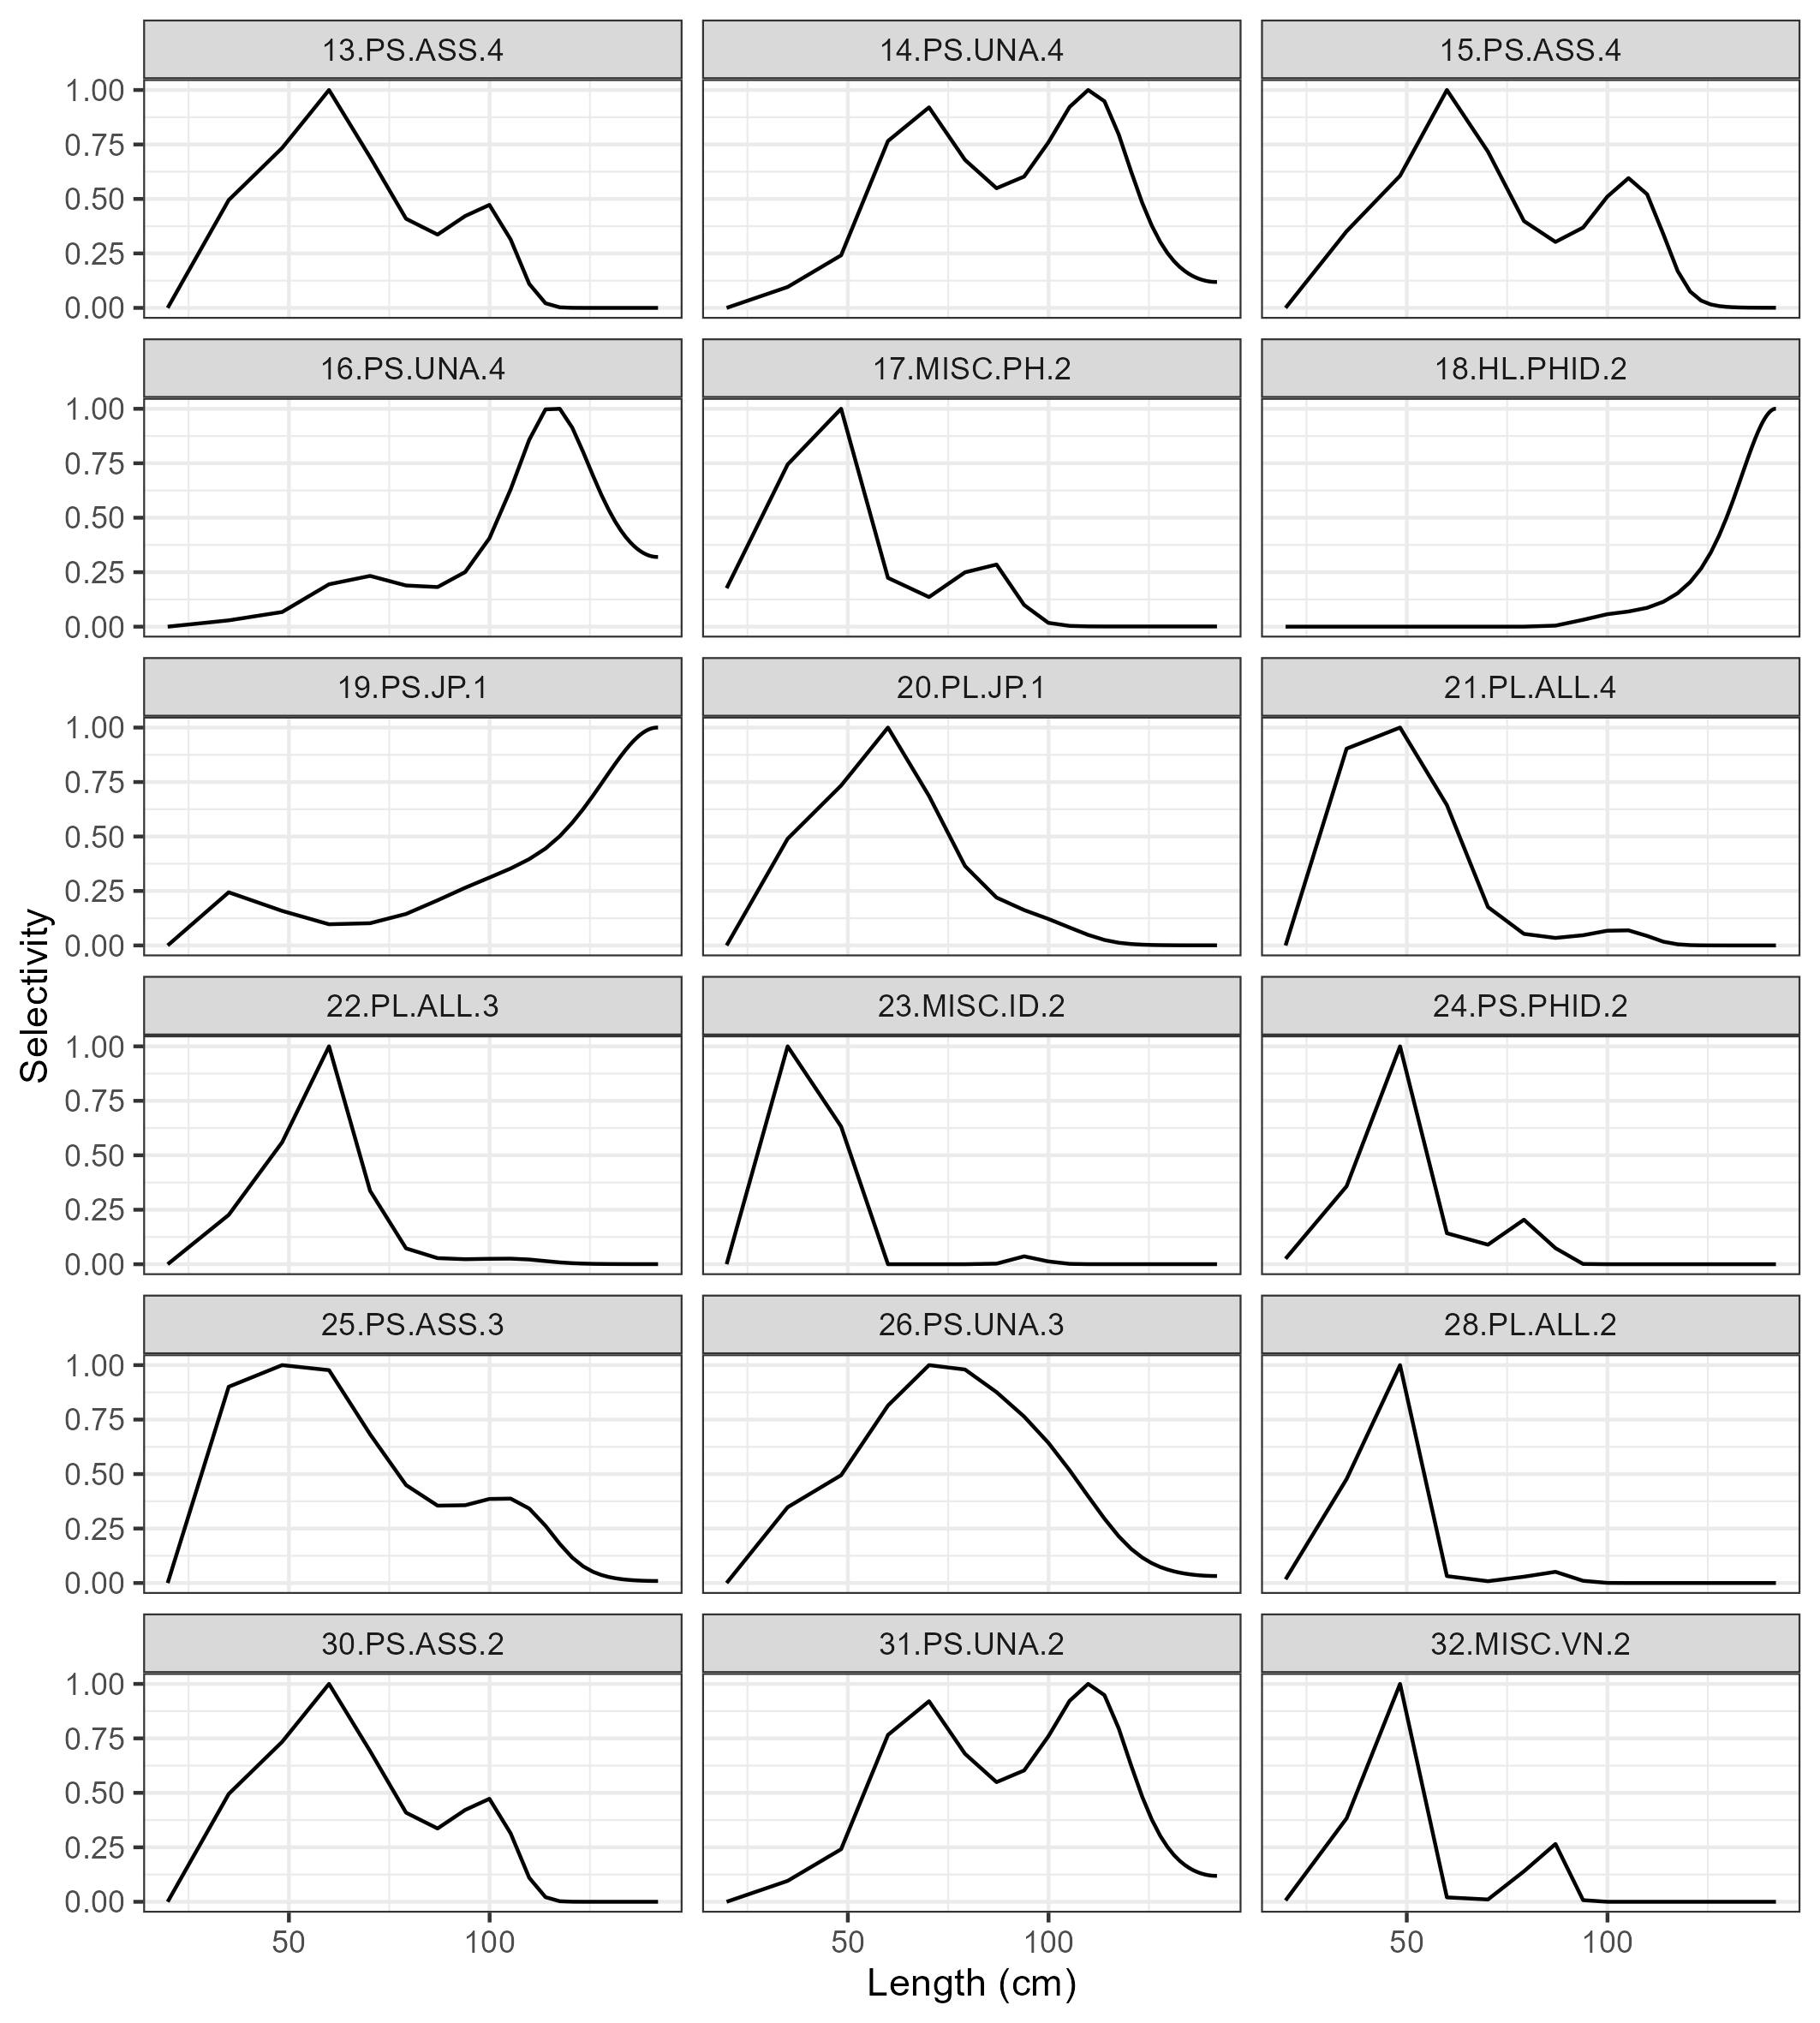
\includegraphics[width=\textwidth]{select_other_length.png}
  \caption{Length-specific selectivity coefficients by groups of fisheries with shared selectivities for miscellaneous and pole and line fisheries. \label{fig:select_other_length}}
\end{figure}
\clearpage

\newpage
\begin{figure}[!ht]
  \centering
  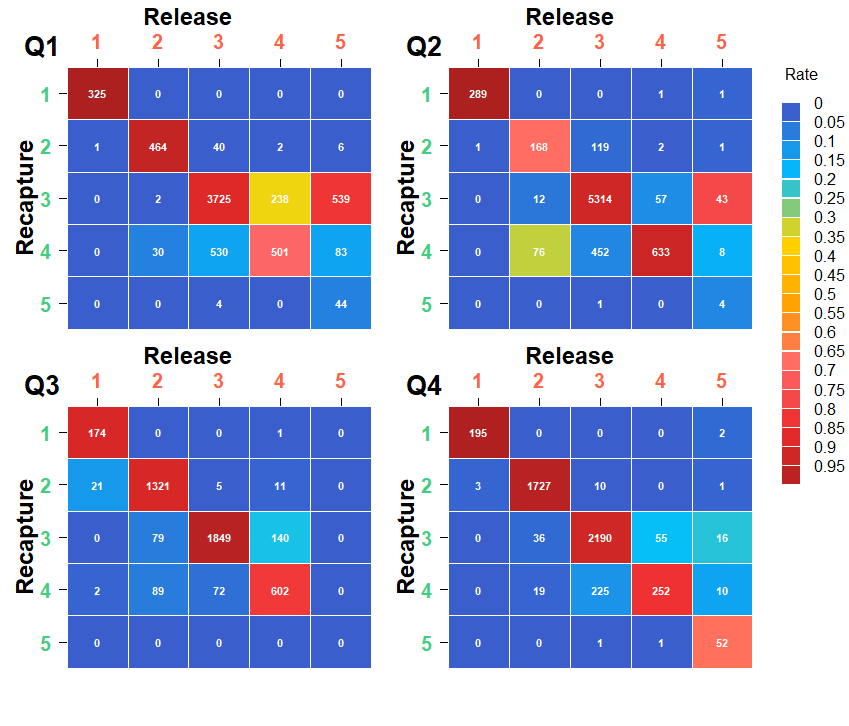
\includegraphics[width=.65\textwidth]{movement_matrix_tag.png}
  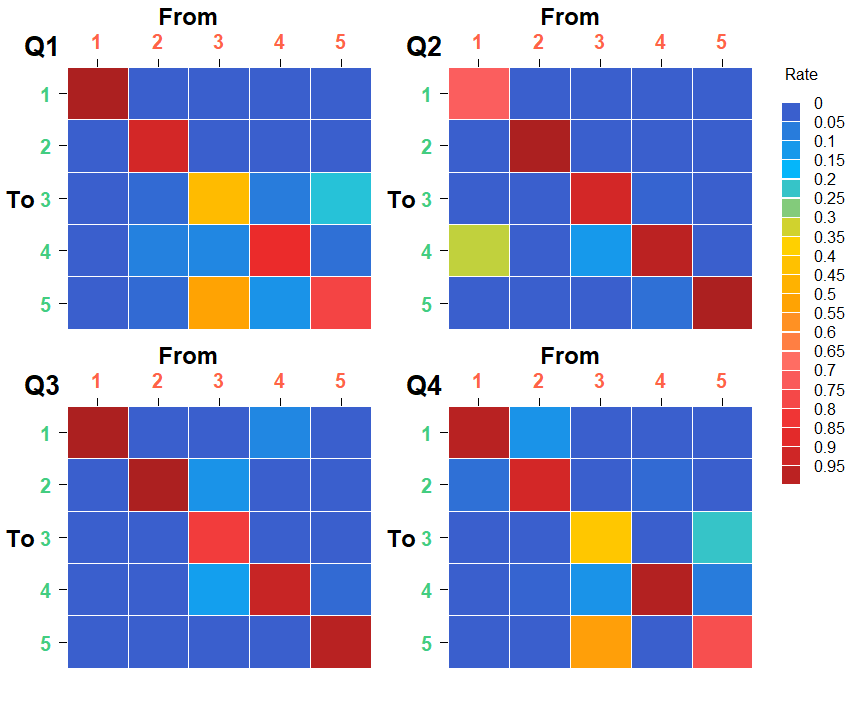
\includegraphics[width=.65\textwidth]{movement_matrix_model.png}
  \caption{(Top) Observed proportion of tags returned by region of release (columns), region of recapture (rows), and quarter of recapture (panel) where the color of the tile indicates the proportion of tags returned from the region of releases, numbers in boxes indicate the actual numbers. (Bottom) Estimated movement probabilities by quarter for the diagnostic case model. The red numbers (horizontal axis) indicate the source model region (From) and the green numbers (vertical axis) indicate the receiving (To) regions. The color of the tile shows the magnitude of the movement rate (proportion of individuals moving from region x to region y in that quarter), with each column adding up to 1. \label{fig:movement_matrices}}
\end{figure}
\clearpage

\newpage
\begin{figure}[!ht]
  \centering
  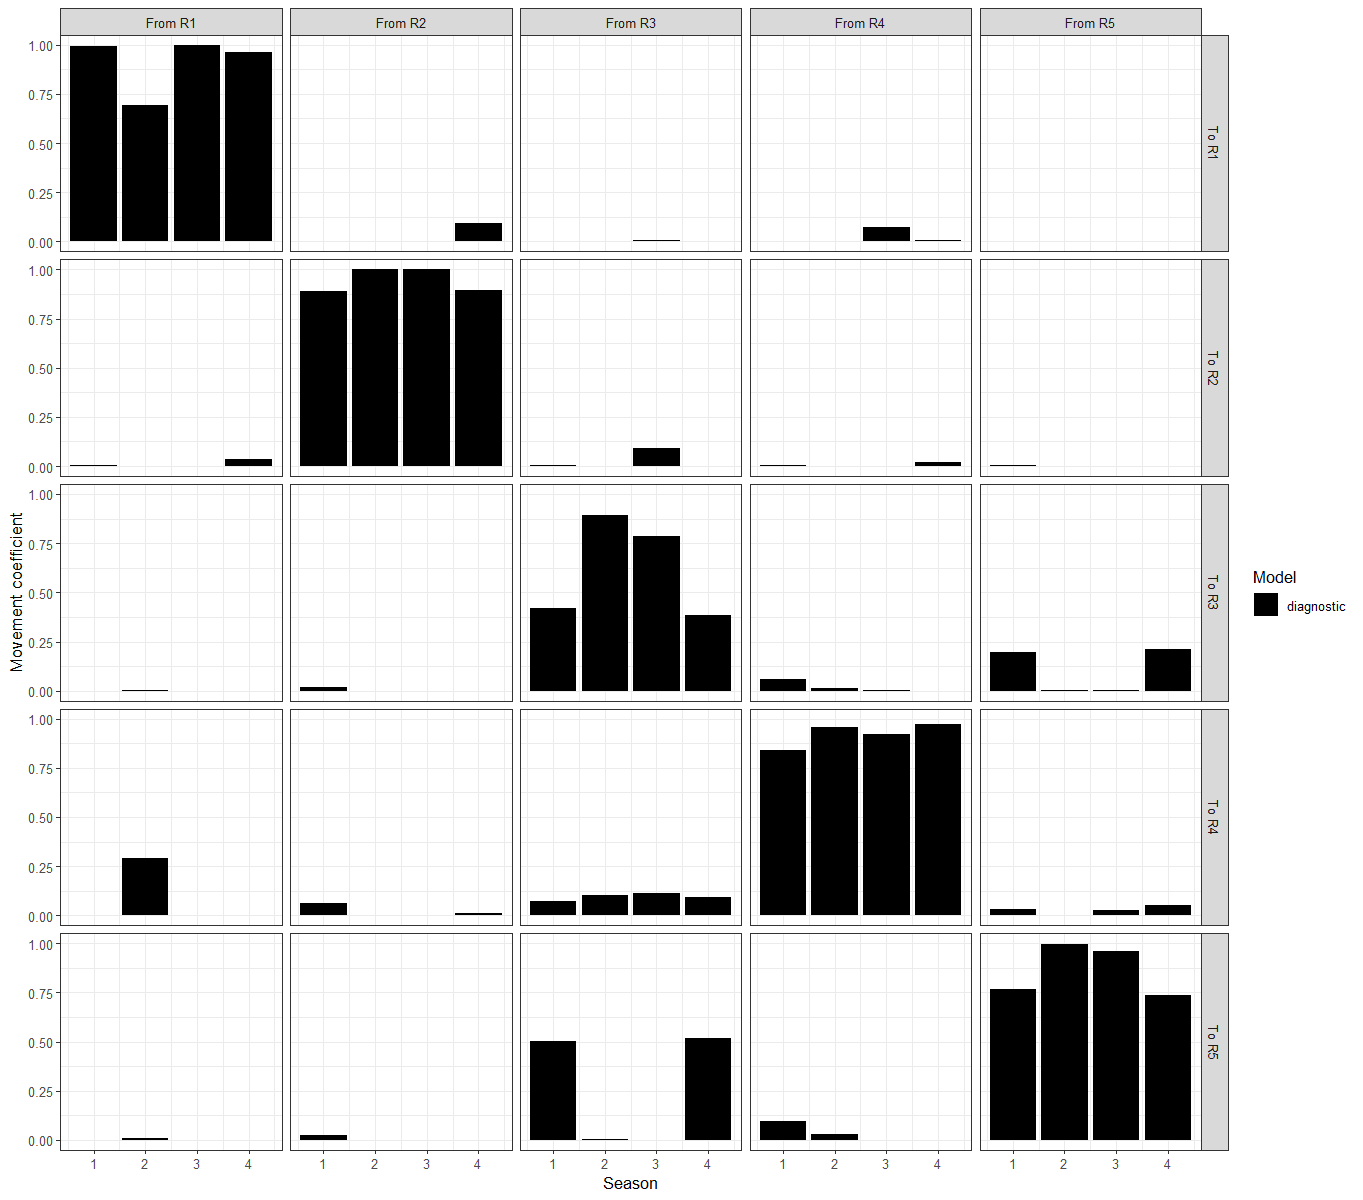
\includegraphics[width=\textwidth]{movement_model_bar_plots.png}
  \caption{Season-specific movement probabilities estimated by the diagnostic model. \label{fig:season_movement_coeff}}
\end{figure}
\clearpage

\newpage
\begin{figure}[!ht]
  \centering
  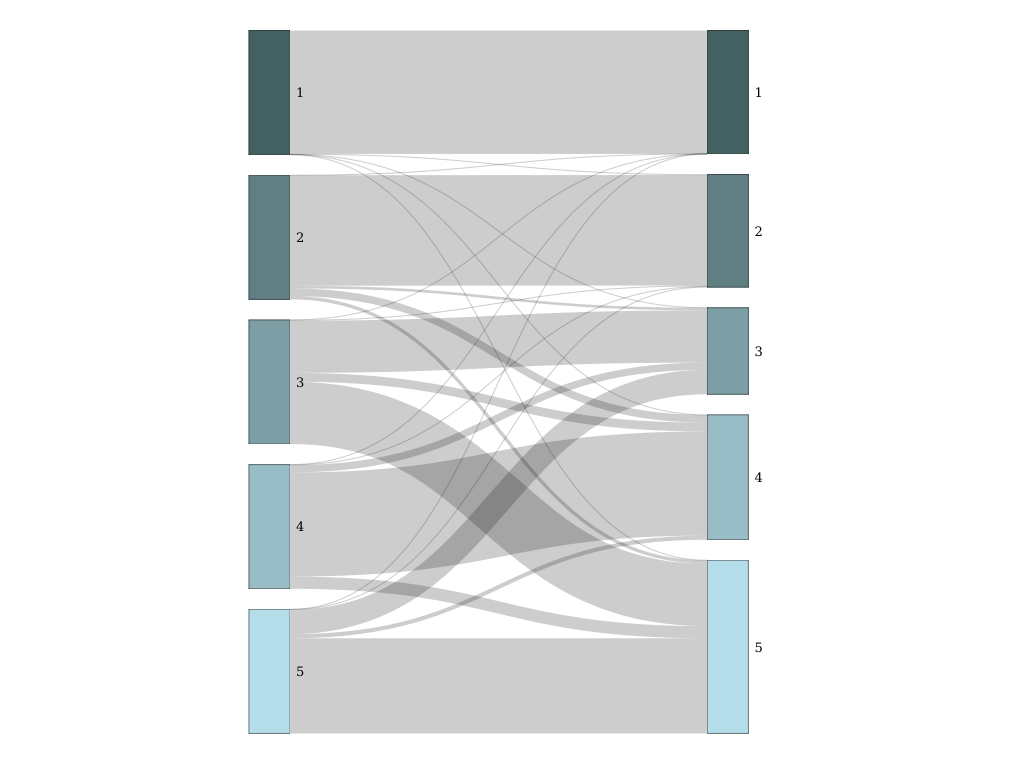
\includegraphics[width=1.1\textwidth]{movement_sankey.png}
  \caption{Stylised estimated movement rates between stock assessment regions (all ages and seasons) for the diagnostic case. Estimated movement is shown FROM the model regions on the left TO the model regions on the right. \label{fig:sankey_movement}}
\end{figure}
\clearpage

\newpage
\begin{figure}[!ht]
  \centering
  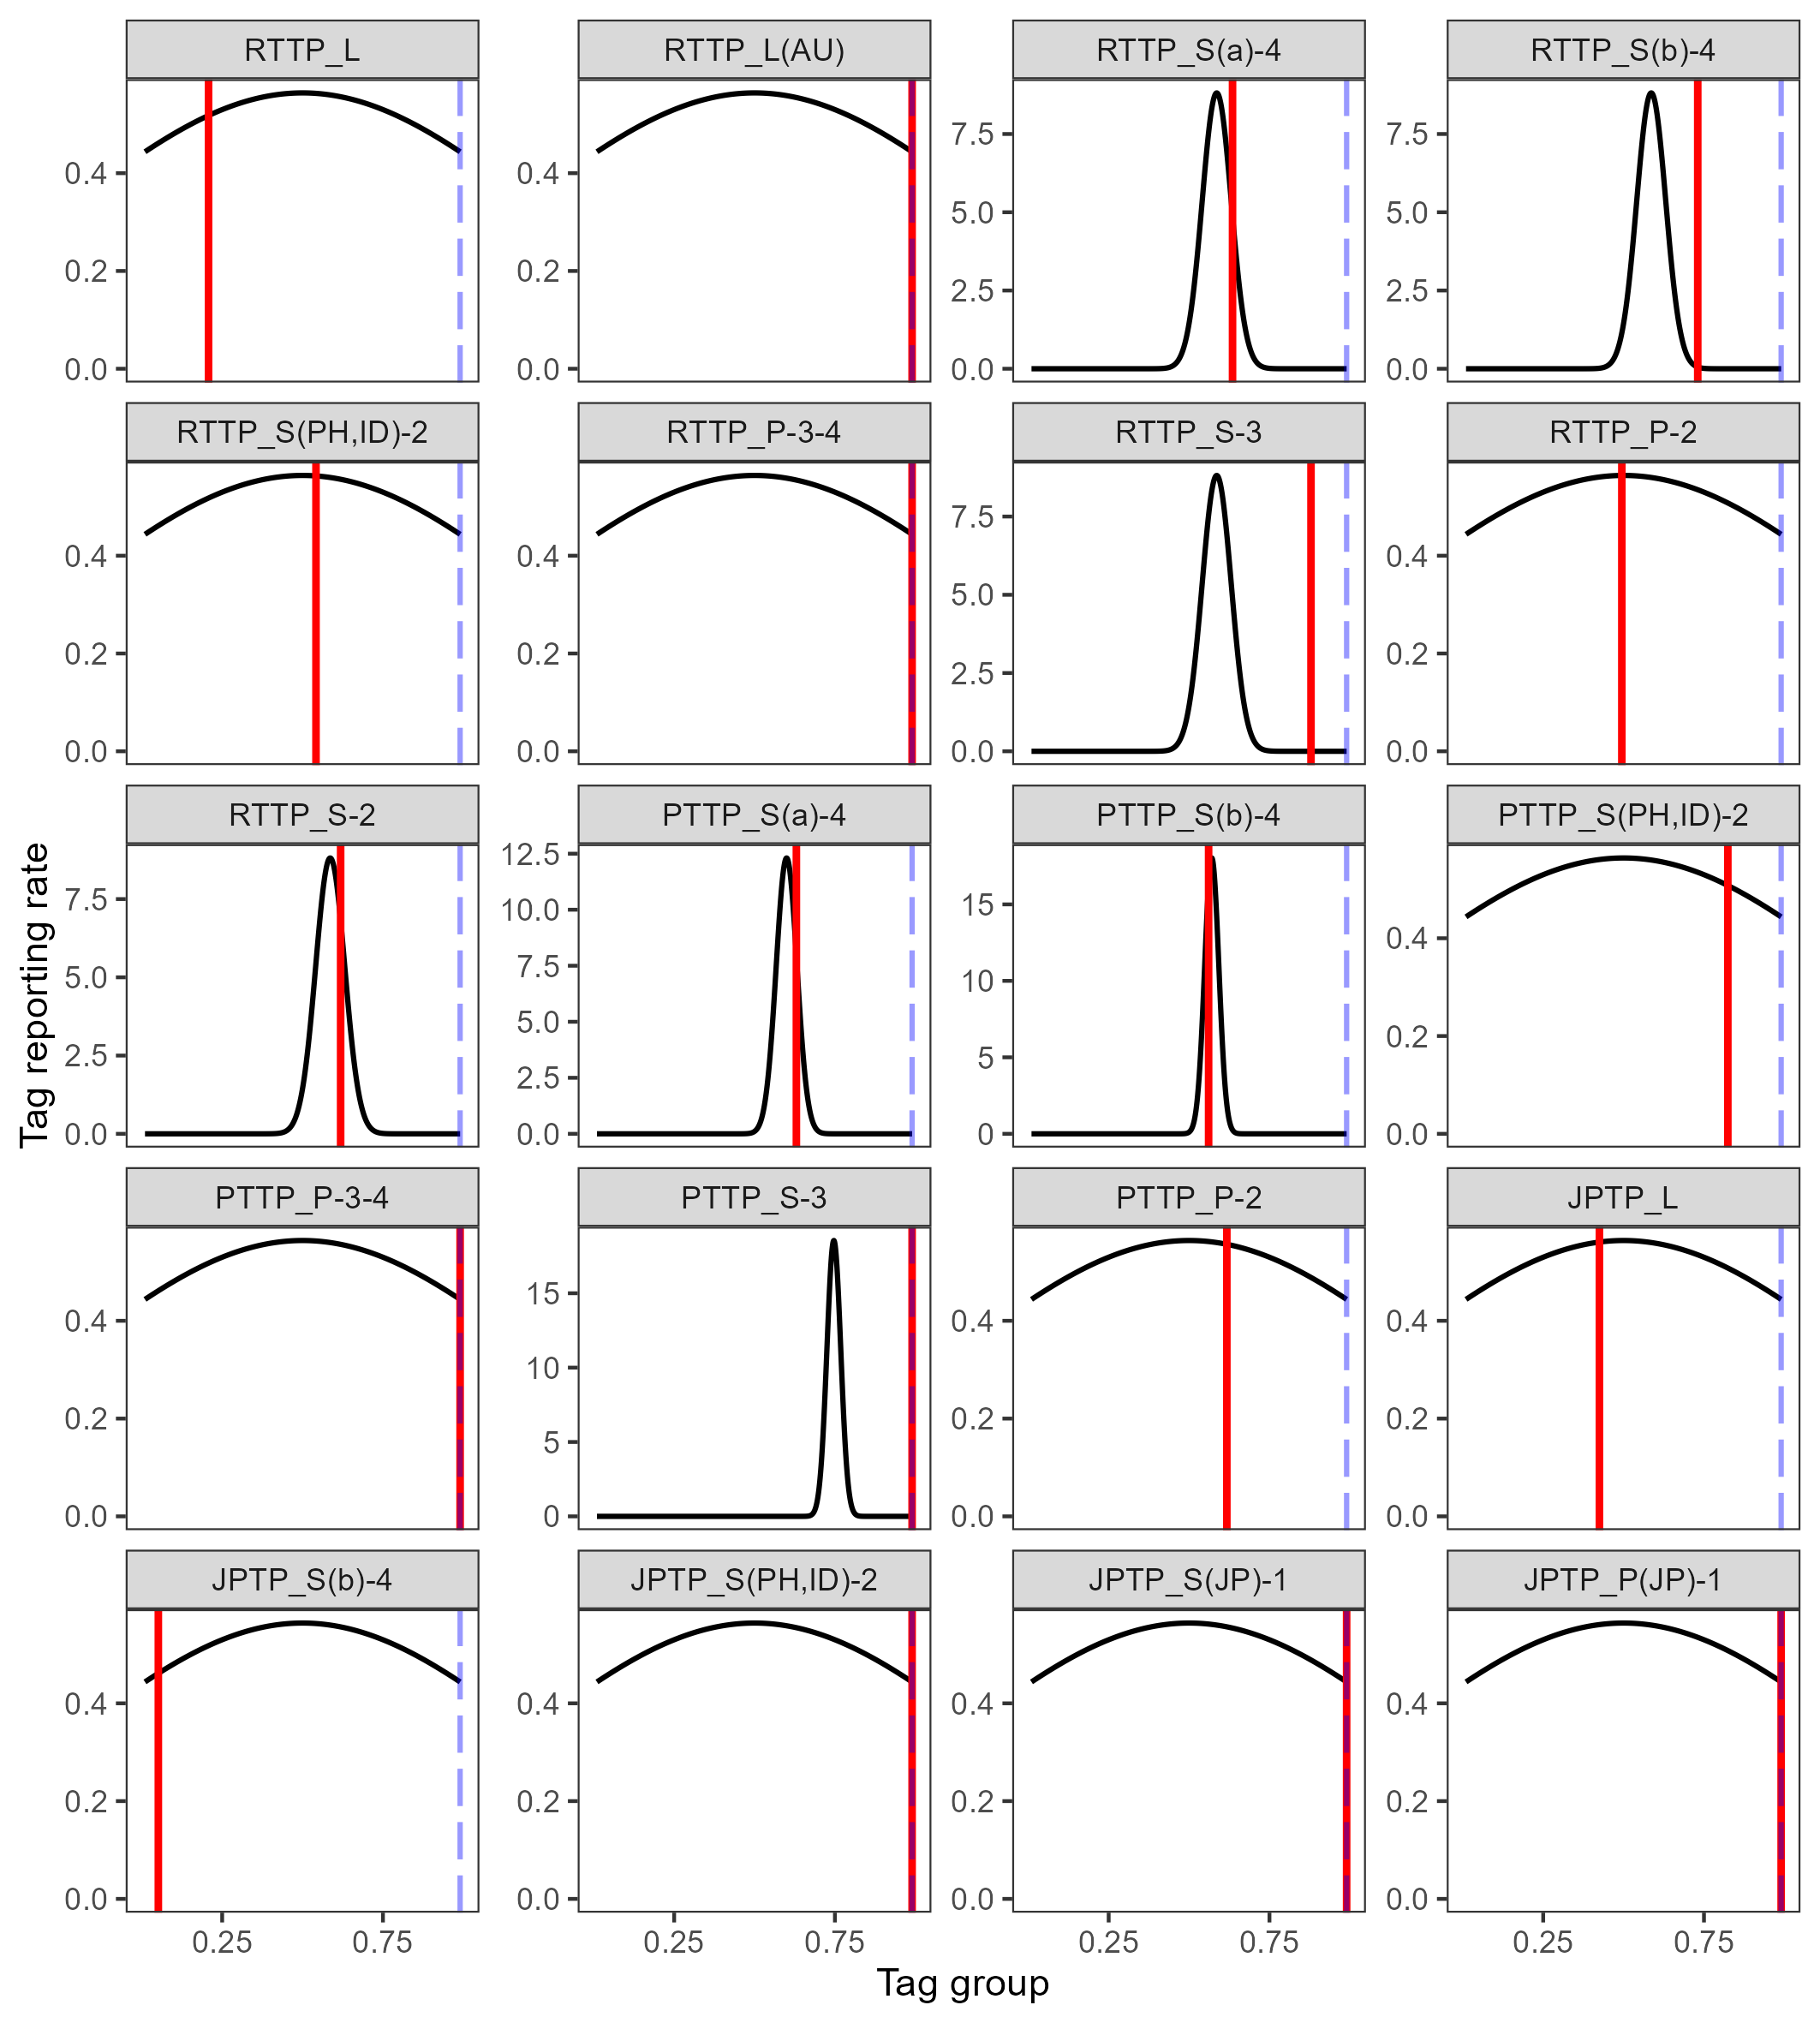
\includegraphics[width=\textwidth]{tag_report_rates.png}
  \caption{Estimated reporting rates for the diagnostic model (red lines) and the prior distribution for each reporting rate group (black lines). The imposed upper bound (0.99) on the reporting rate parameters is shown as a blue dashed line. Reporting rates can be estimated separately for each release program and recapture fishery group but in practice are aggregated over some recapture groups to reduce dimensionality. \label{fig:tag_report_rates}}
\end{figure}
\clearpage

\newpage
\begin{figure}[!ht]
  \centering
  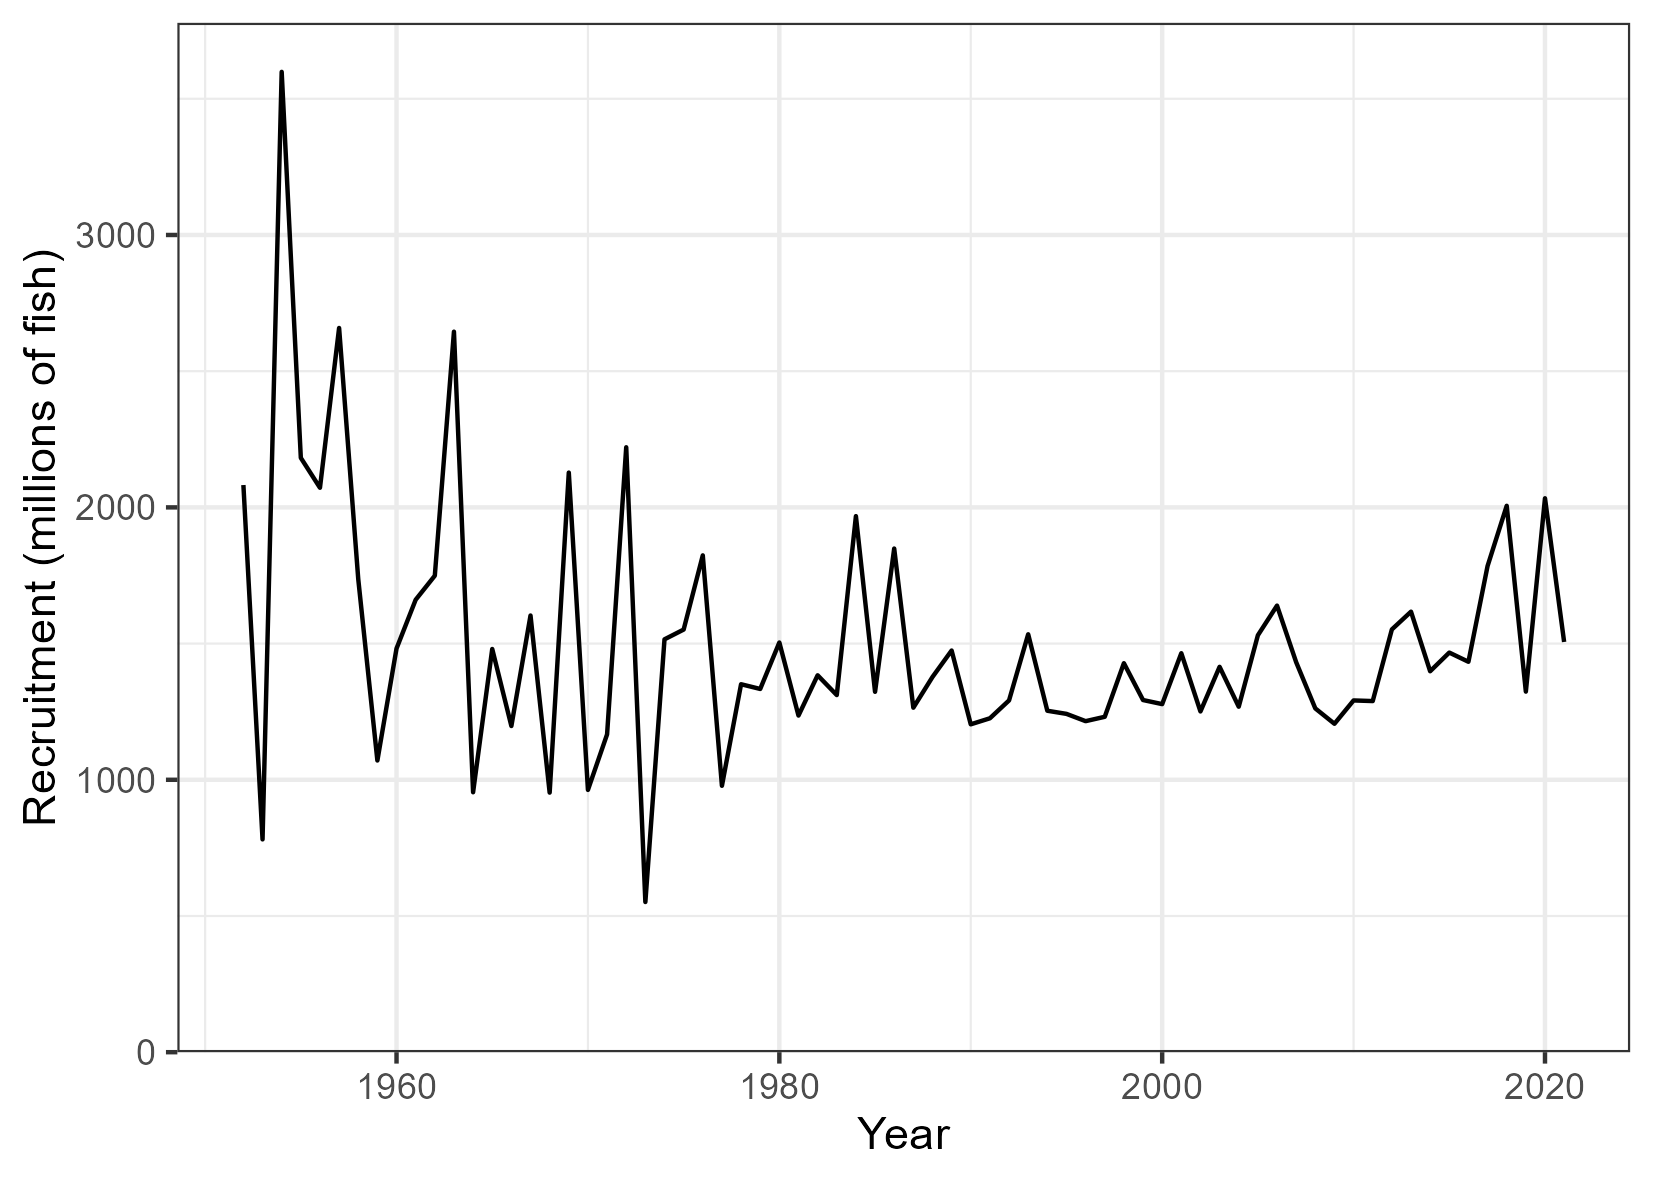
\includegraphics[width=0.9\textwidth]{recruitment_annual_all.png}
  \caption{Time series of estimated annual recruitment summed across regions for the diagnostic model.\label{fig:recruitment_annual_all}}
\end{figure}
\clearpage

\newpage
\begin{figure}[!ht]
  \centering
  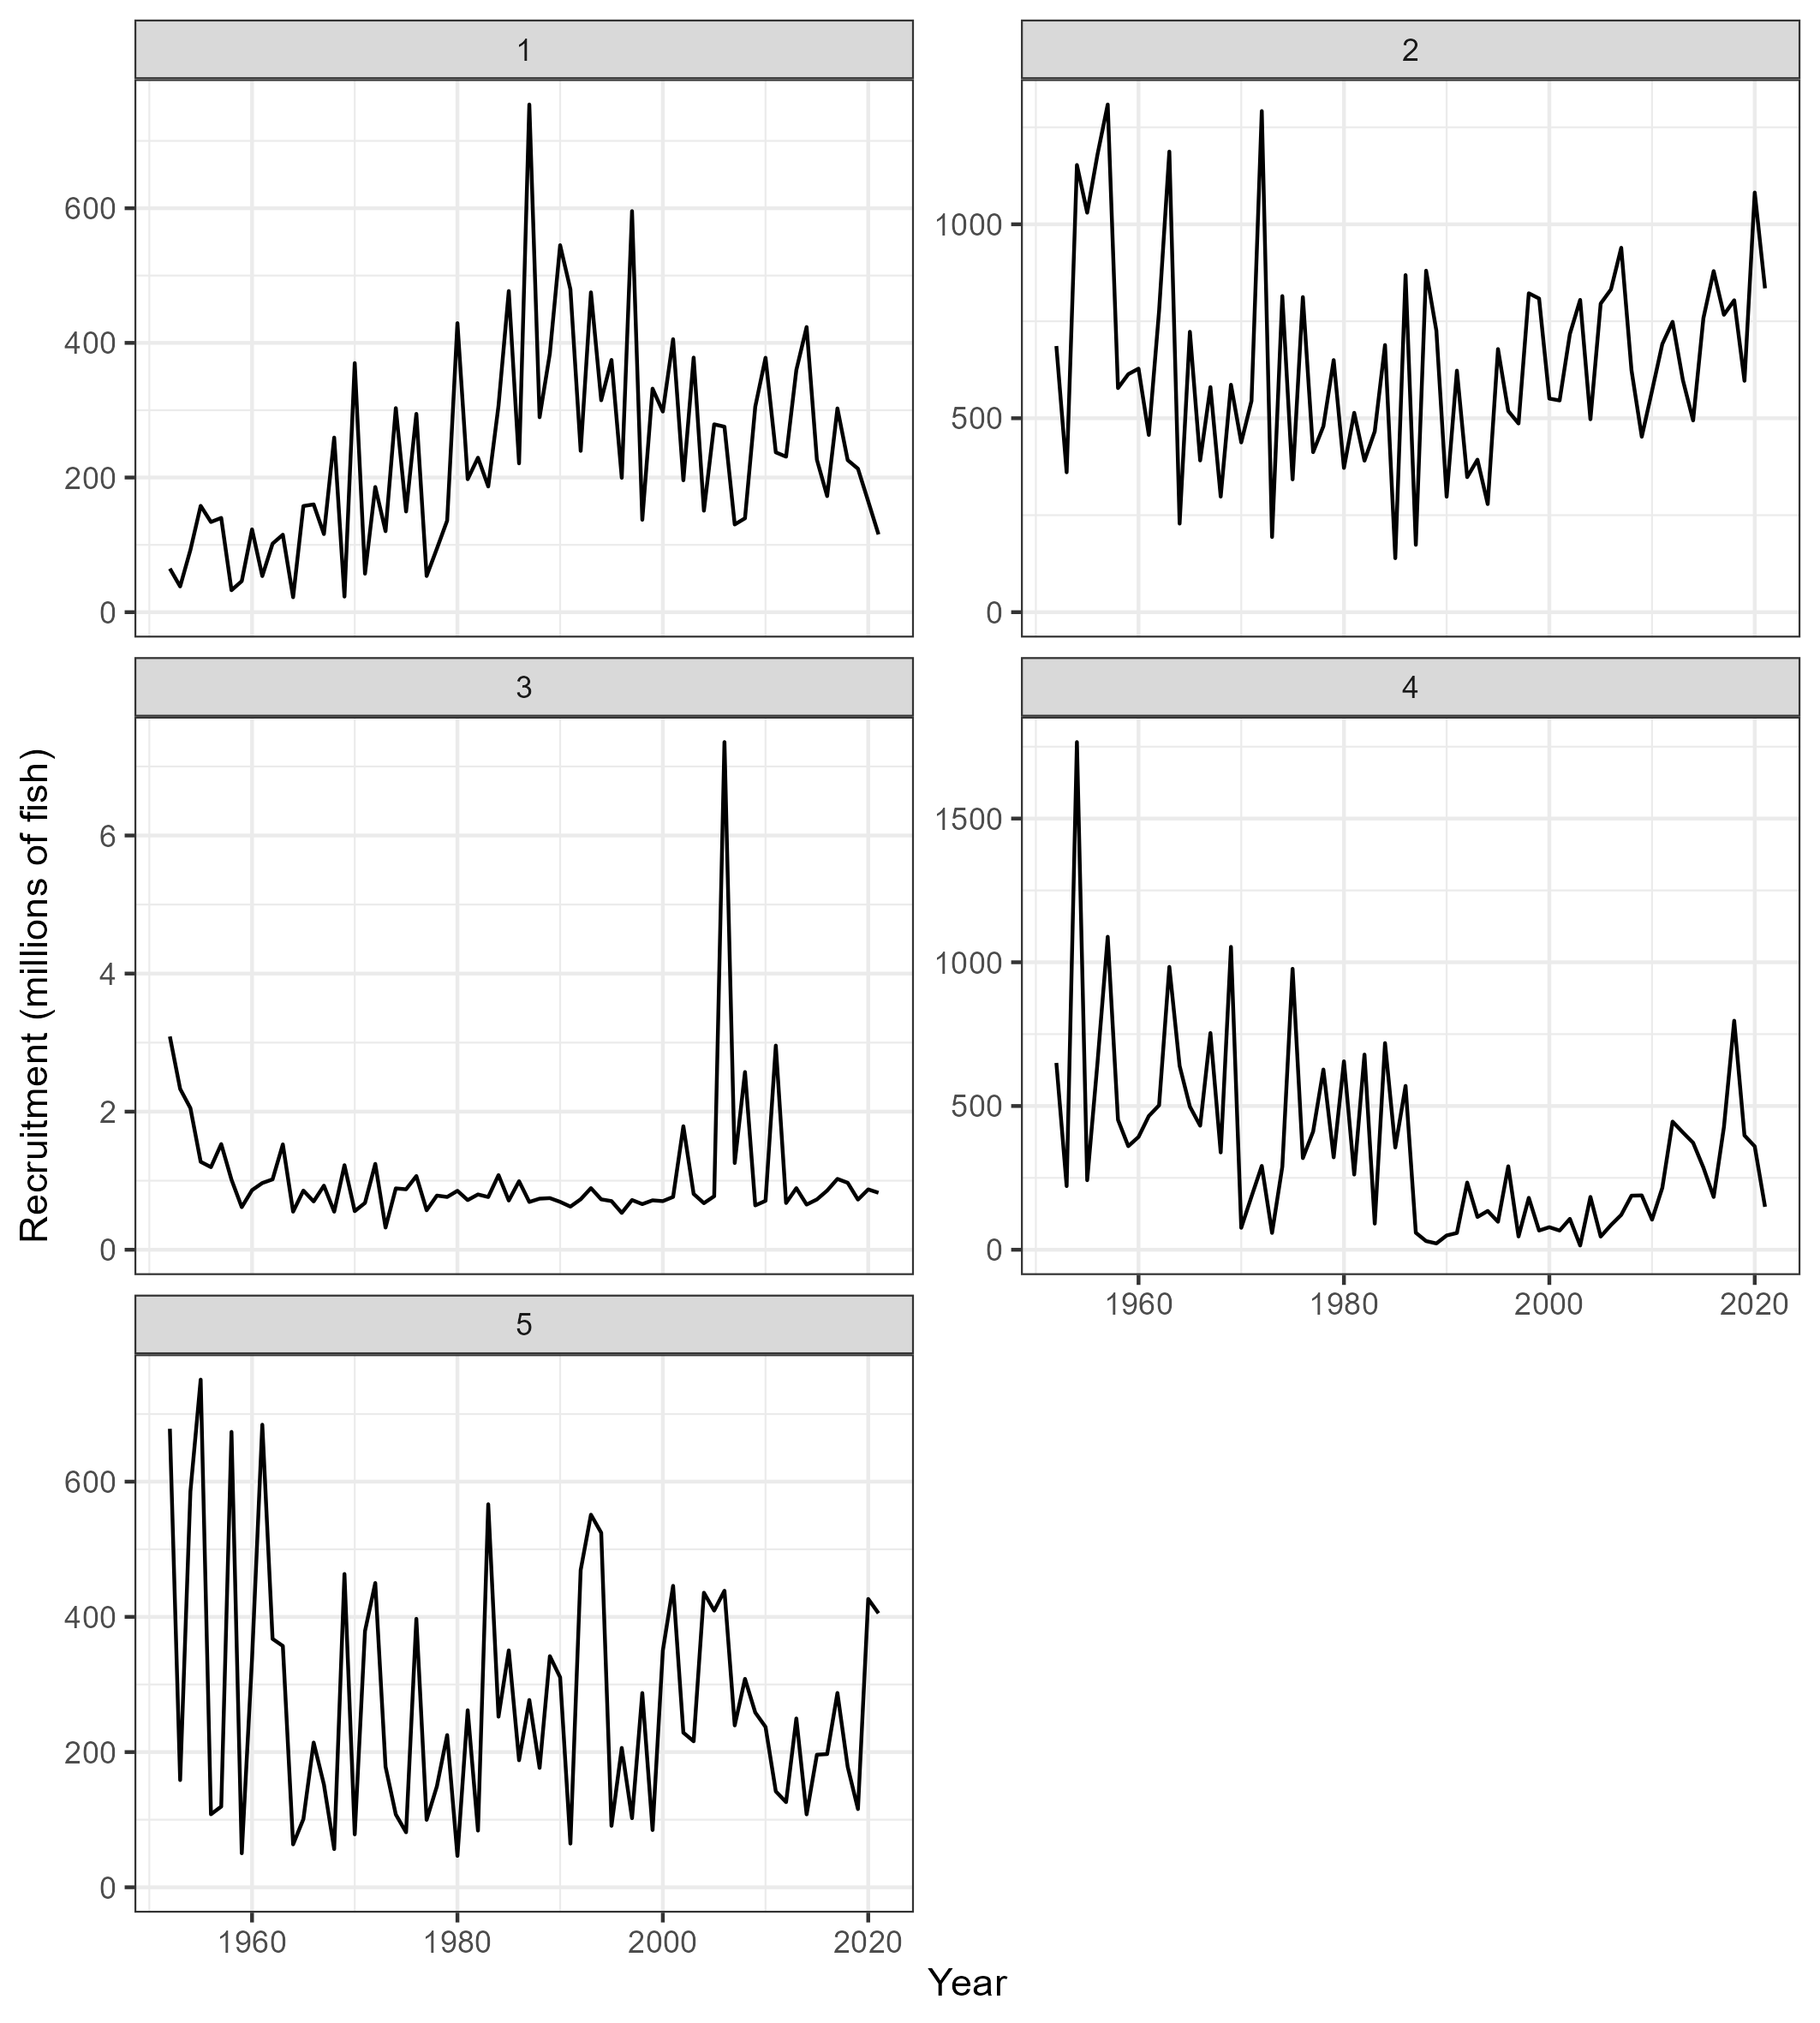
\includegraphics[width=\textwidth]{recruitment_annual_regions.png}
  \caption{Time series of estimated annual recruitment by model region for the diagnostic model. Note that the scale of the y-axis is not constant across regions.\label{fig:recruitment_annual_regions}}
\end{figure}
\clearpage

\newpage
\begin{figure}[!ht]
  \centering
  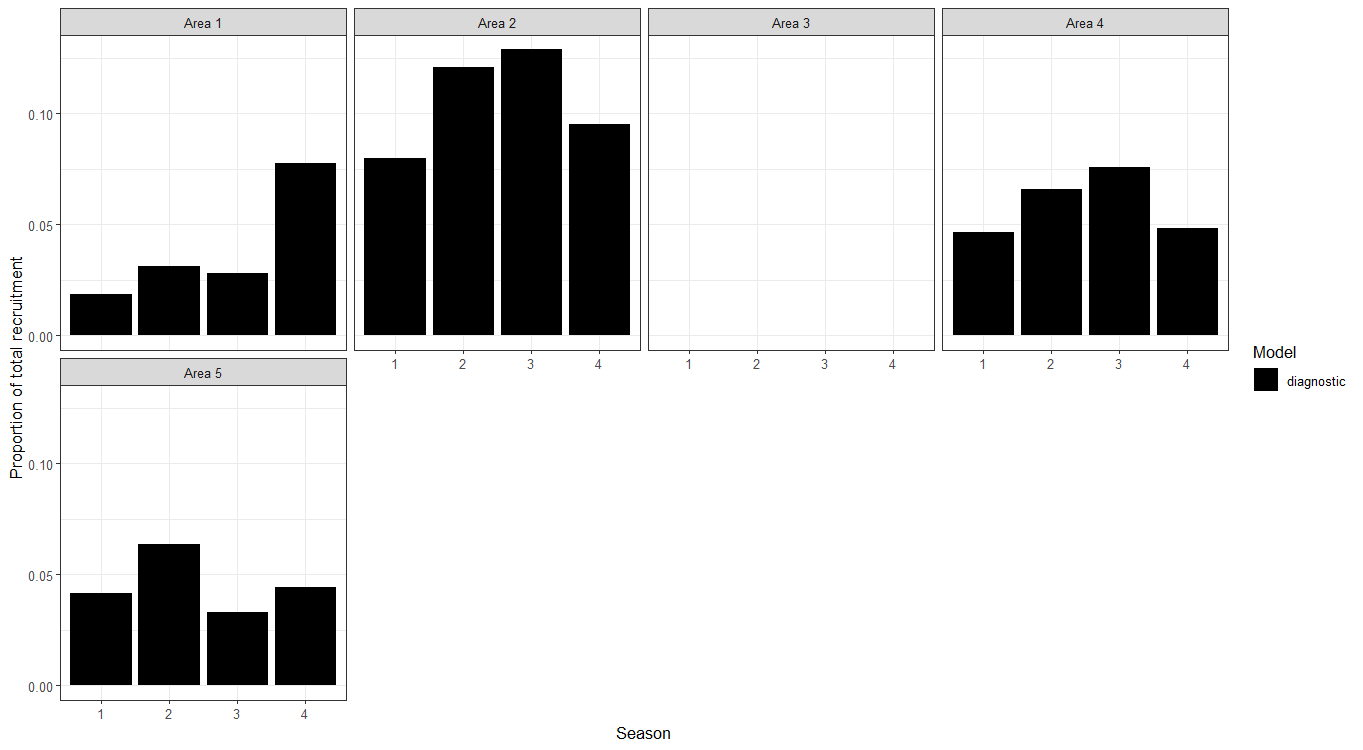
\includegraphics[width=\textwidth]{proportion_rec_region_qutr.png}
  \caption{Estimated recruitment distribution by region and quarter. \label{fig:proportion_rec_region_qutr}}
\end{figure}

\begin{figure}[!ht]
  \centering
  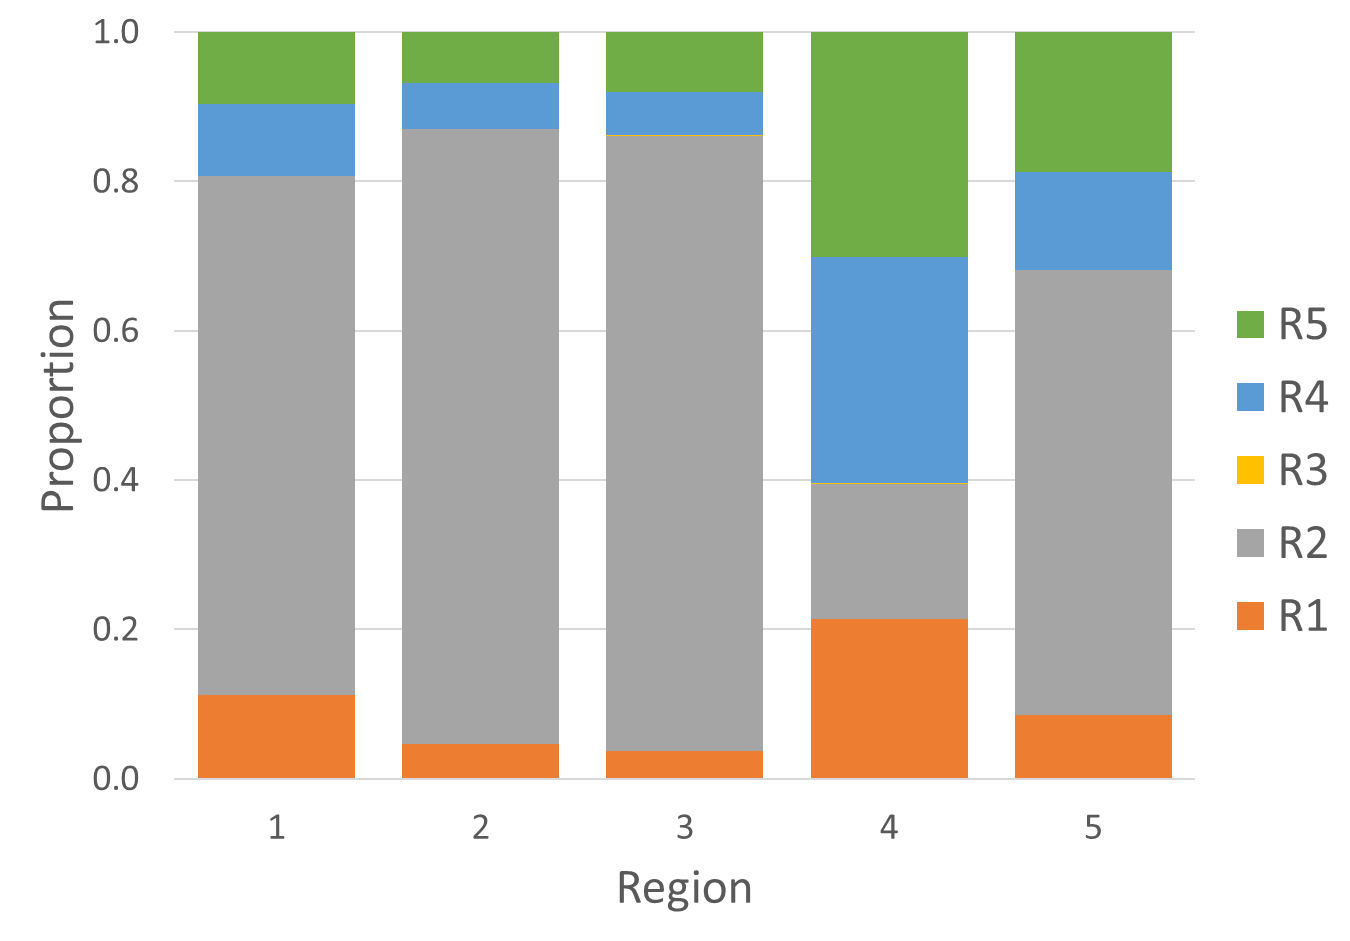
\includegraphics[width=0.9\textwidth]{proportions_biomass_by_source_fmult0.png}
  \caption{Proportional distribution of unfished total biomass in each region apportioned by the source region of the fish, for the diagnostic model. The colour of the originating region is presented in the legend. The biomass distributions are calculated based on the long-term average distribution of recruitment between regions, estimated movement parameters, and natural mortality. \label{fig:proportions_biomass_by_source_fmult0}}
\end{figure}
\clearpage

\newpage
\begin{figure}[!ht]
  \centering
  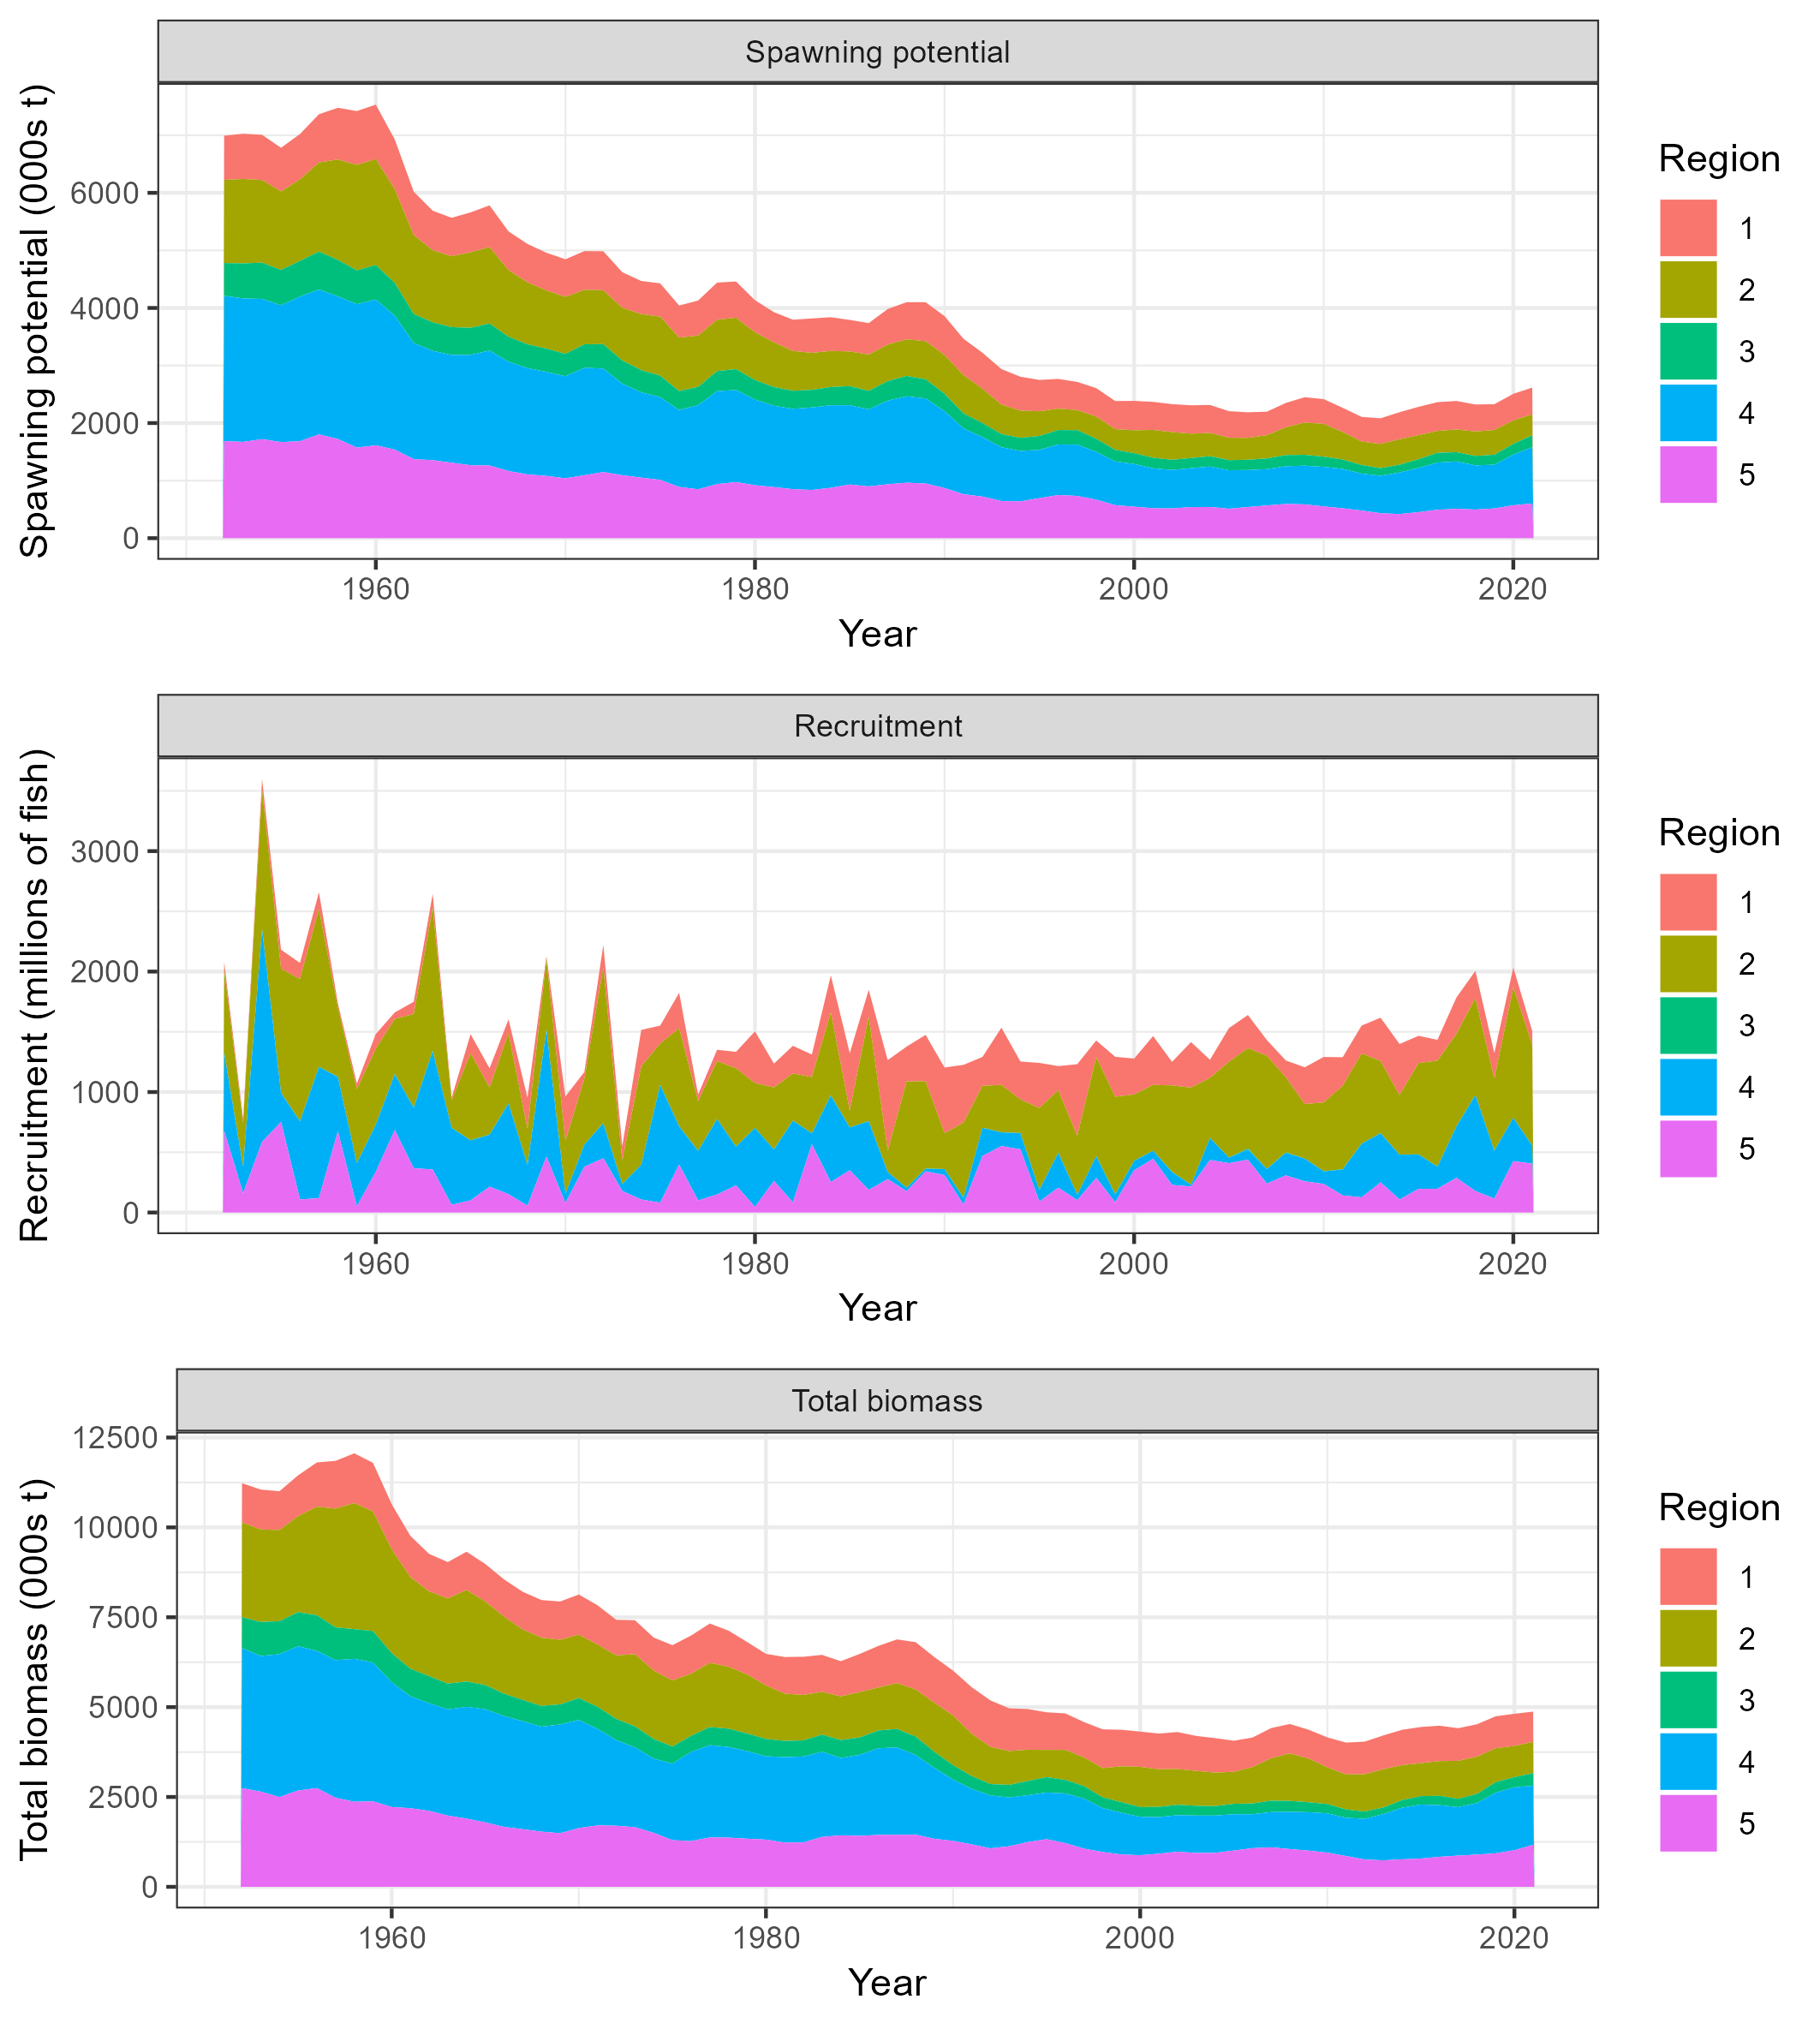
\includegraphics[width=\textwidth]{spawnpot_rec_biomass_panel.png}
  \caption{Time series of estimated annual spawning potential, recruitment and total biomass by model region for the diagnostic model, showing the relative proportions among regions. Note the data represent the averages of the quarterly model time steps for each year for spawning potential and total biomass and the sum of the quarterly recruitment estimates for annual recruitment. \label{fig:spawnpot_rec_biomass_panel}}
\end{figure}
\clearpage

\newpage
\begin{figure}[!ht]
  \centering
  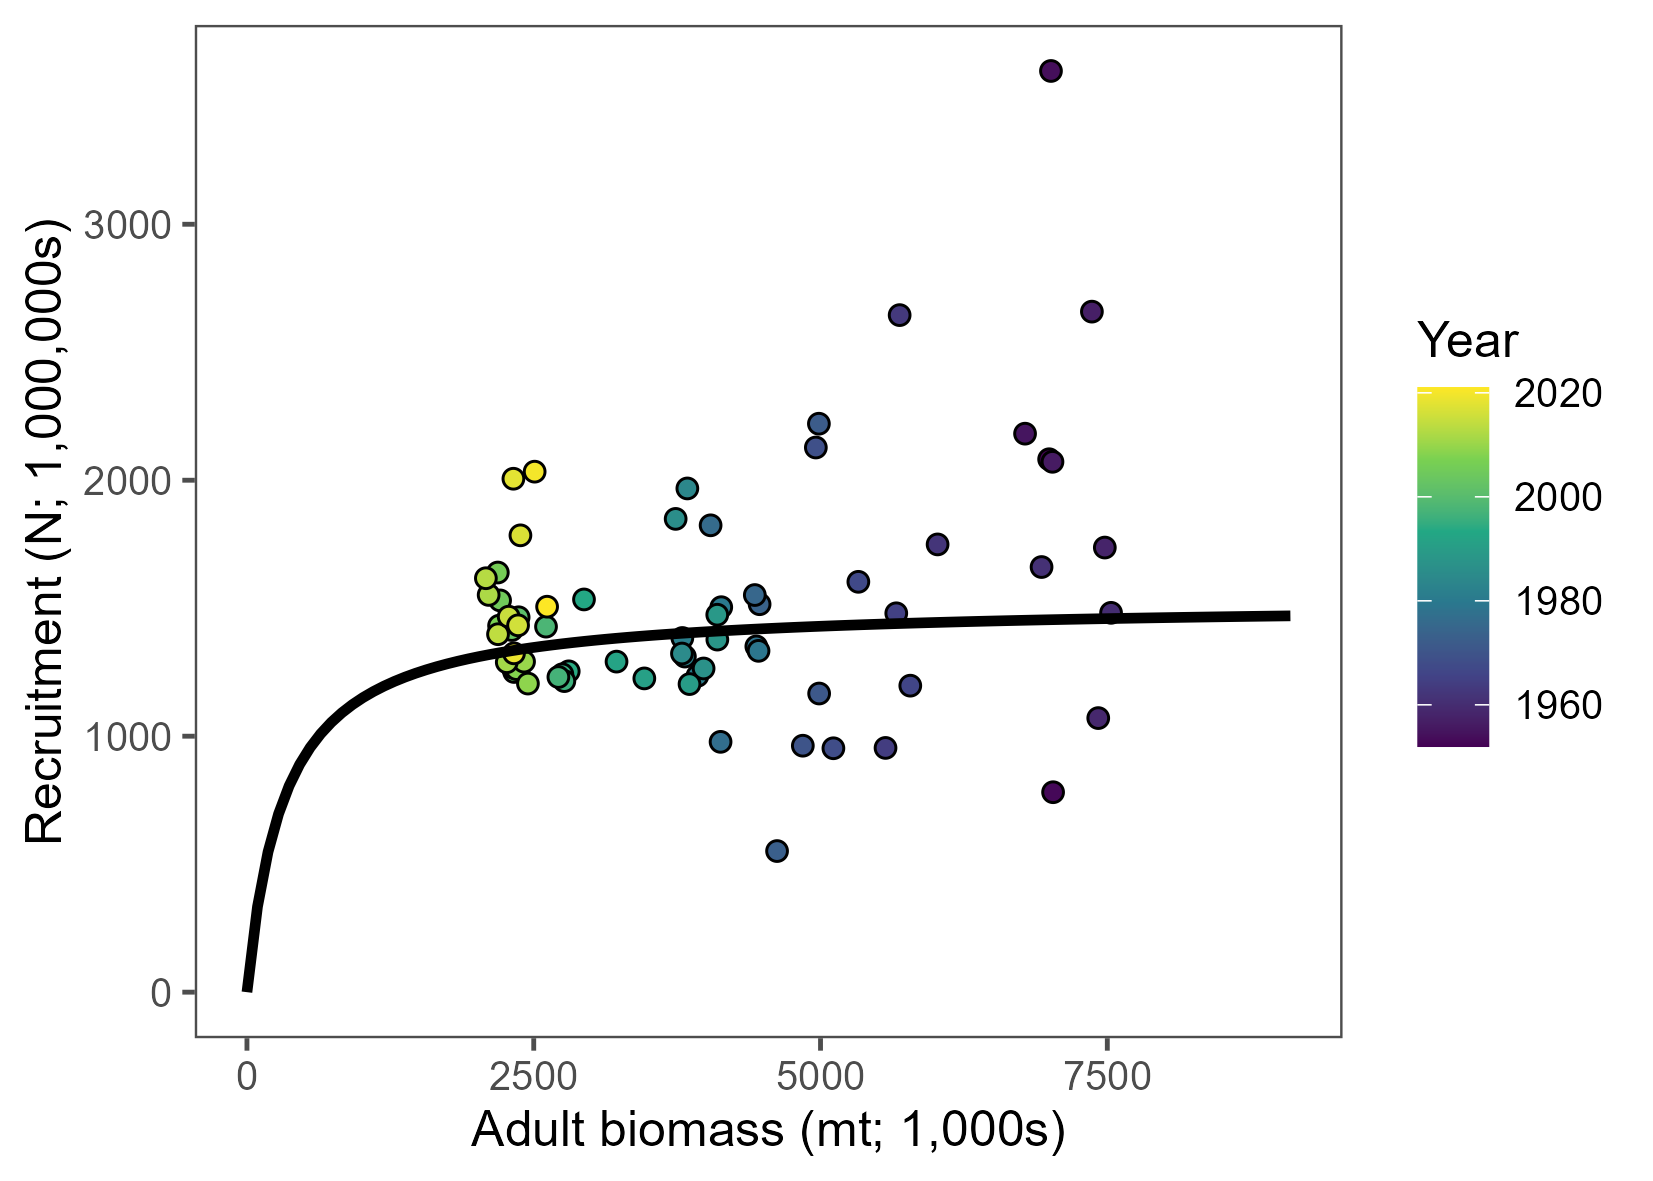
\includegraphics[width=0.8\textwidth]{stock_RR.png}
  \caption{Estimated relationship between recruitment and spawning potential based on annual values for the diagnostic model. The darkness of the circles changes from light (more recent) to darker (earlier) through time.\label{fig:stock_RR}}
\end{figure}
\clearpage

\newpage
\begin{figure}[!ht]
  \centering
  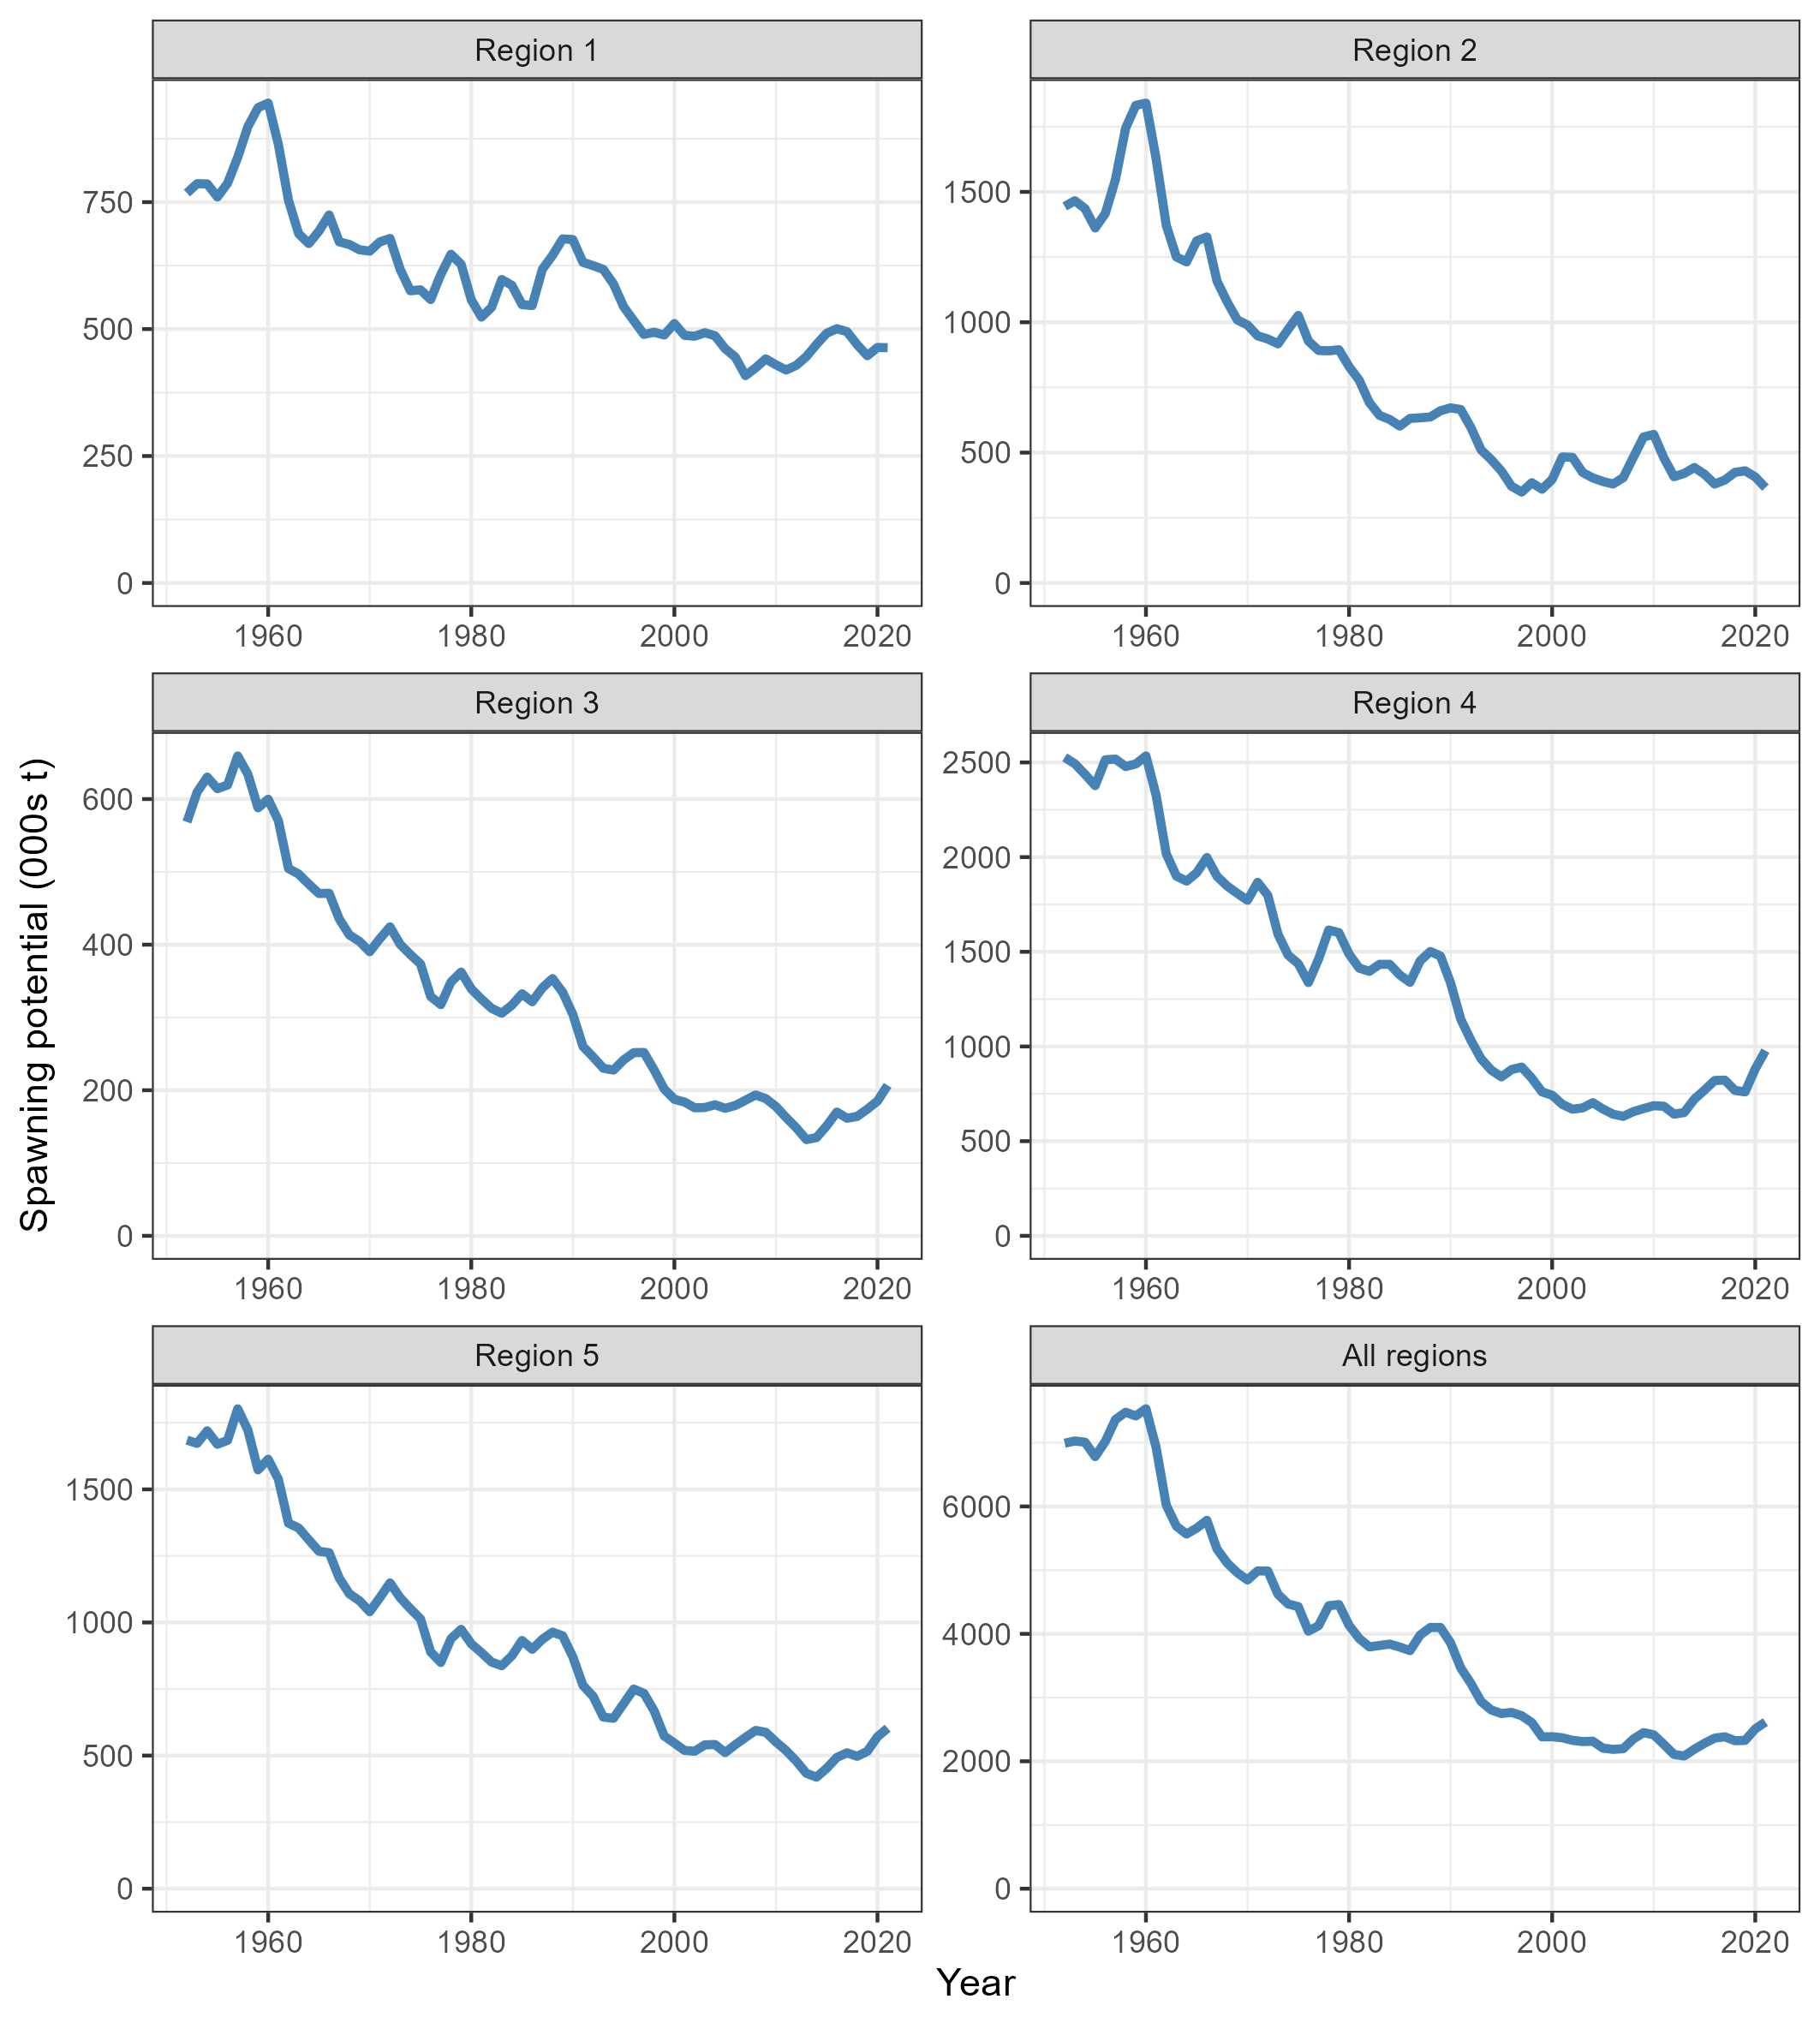
\includegraphics[width=\textwidth]{spawnpotential_annual_region_diag.png}
  \caption{Estimated temporal spawning potential, \sbt, by model region, and for all model regions summed for the diagnostic model. Note that the scale of the y-axis is not constant across regions.\label{fig:spawnpotential_annual_region_diag}}
\end{figure}
\clearpage

\newpage
\begin{figure}[!ht]
  \centering
  \includegraphics[width=\textwidth]{depletion_annual_region_diag.png}
  \caption{Estimated temporal spawning potential depletion, \sbtsbfo, by model region, and for all model regions summed for the diagnostic model. \label{fig:depletion_annual_region_diag}}
\end{figure}
\clearpage

\newpage
\begin{figure}[!ht]
  \centering
  \includegraphics[width=\textwidth]{fished_unfished_SB.png}
  \caption{Comparison of the estimated annual spawning potential trajectories (lower blue lines) with the spawning potential trajectories predicted to have occurred in the absence of fishing (upper red lines) for each region and overall, for the diagnostic model. Note the scales of the Y-axes vary. \label{fig:fished_unfished_SB}}
\end{figure}
\clearpage

\newpage
\begin{figure}[!ht]
  \centering
  \includegraphics[width=0.9\textwidth]{juv_adult_F.png}
  \caption{Estimated annual average adult (solid line) and juvenile (dashed line) fishing mortality for the diagnostic model.\label{fig:juv_adult_F}}
\end{figure}
\clearpage

\newpage
\begin{figure}[!ht]
  \centering
  \includegraphics[width=\textwidth]{age_specific_F.png}
  \caption{Estimated age-specific fishing mortality for the diagnostic model, by region and overall.\label{fig:age_specific_F}}
\end{figure}
\clearpage

\newpage
\begin{figure}[!ht]
  \centering
  \includegraphics[width=\textwidth]{prop_at_age_F_by_decades.png}
  \caption{Estimated proportion at age (quarters) and fishing mortality at age (right), by year, at decade intervals, for the diagnostic model.\label{fig:prop_at_age_F_by_decades}}
\end{figure}
\clearpage

\newpage
\begin{figure}[!ht]
  \centering
  \includegraphics[width=0.75\textwidth]{oneoff_tagmix_depletion.png}\\[4mm]
  \includegraphics[width=0.75\textwidth]{oneoff_tagmix_sb.png}
  \caption{Estimated dynamic spawning depletion (top) and spawning potential (bottom) for the one-off sensitivities from the 2023 diagnostic model for tag mixing period. m=tag mixing, h=steepness, s=size data, a=age data.\label{fig:one_off_sens_tagmix}}
\end{figure}
\clearpage

\newpage
\begin{figure}[!ht]
  \centering
  \includegraphics[width=0.75\textwidth]{oneoff_steepness_depletion.png}\\[4mm]
  \includegraphics[width=0.75\textwidth]{oneoff_steepness_sb.png}
  \caption{Estimated dynamic spawning depletion (top) and spawning potential (bottom) for the one-off sensitivities from the 2023 diagnostic model for steepness of the stock recruitment relationship. m=tag mixing, h=steepness, s=size data, a=age data.\label{fig:one_off_sens_steepness}}
\end{figure}
\clearpage

\newpage
\begin{figure}[!ht]
  \centering
  \includegraphics[width=0.75\textwidth]{oneoff_sizedatawt_depletion.png}\\[4mm]
  \includegraphics[width=0.75\textwidth]{oneoff_sizedatawt_sb.png}
  \caption{Estimated dynamic spawning depletion (top) and spawning potential (bottom) for the one-off sensitivities from the 2023 diagnostic model for size data weighting. m=tag mixing, h=steepness, s=size data, a=age data.\label{fig:one_off_sens_sizedatawt}}
\end{figure}
\clearpage

\newpage
\begin{figure}[!ht]
  \centering
  \includegraphics[width=0.75\textwidth]{oneoff_agedatawt_depletion.png}\\[4mm]
  \includegraphics[width=0.75\textwidth]{oneoff_agedatawt_sb.png}
  \caption{Estimated dynamic spawning depletion (top) and spawning potential (bottom) for the one-off sensitivities from the 2023 diagnostic model for age data weighting. m=tag mixing, h=steepness, s=size data, a=age data. \label{fig:one_off_sens_agedatawt}}
\end{figure}
\clearpage

\newpage
\begin{figure}[!ht]
  \centering
  \includegraphics[width=1\textwidth]{violin_grid_MSY_depletion.png}
  \caption{Box and violin plots summarizing the estimated \fref (top) and \sbrsbfo (bottom) for each of the models in the structural uncertainty grid grouped by uncertainty axes (steepness, tag mixing, size data weighting, age data weighting). The horizontal lines are the 25th, 50th, and 75th percentiles. The shaded area shows the probability distribution (or density) of the estimates for all models in the structural uncertainty grid. These plots only include the structural uncertainty, not the estimation uncertainty.
    \label{fig:violin_grid_axes}}
\end{figure}
\clearpage

\newpage
\begin{figure}[!ht]
  \centering
  \includegraphics[width=\textwidth]{violin_rec_props_grid.png}
  \caption{Box and violin plots showing the distribution of recruitment across model regions and quarters for all models in the uncertainty grid. The horizontal lines are the 25th, 50th, and 75th percentiles. The shaded area shows the probability distribution (or density) of the estimates of all models of the structural uncertainty grid. These plots only include the structural uncertainty, not the estimation uncertainty.
    \label{fig:violin_rec_props_grid}}
\end{figure}
\clearpage

\newpage
\begin{landscape}
  \begin{figure}[!ht]
    \centering
    \includegraphics[width=0.65\textwidth]{grid_deplet_ind.png}~~~
    \includegraphics[width=0.65\textwidth]{grid_deplet_ribbon.png}
    \caption{(Left) Trajectories of spawning potential depletion for the individual model runs included in the structural uncertainty grid over the period 1952-2021.(Right) Estimated spawning depletion across all models in the structural uncertainty grid over the period 1952-2021. The dashed line represents the median, the lighter band shows the 25th and 75th percentiles, and the dark band shows the 10th and 90th percentiles of the model estimates. The bar at the right of each ribbon indicates the median (black dots) with the 10th and 90th percentiles for \sbrsbfo. \label{fig:grid-depletion}}
  \end{figure}
\end{landscape}
\clearpage

\newpage
\begin{landscape}
  \begin{figure}[!ht]
    \centering
    \includegraphics[width=0.65\textwidth]{grid_SB_ind.png}~~~
    \includegraphics[width=0.65\textwidth]{grid_SB_ribbon.png}
    \caption{(Left) Trajectories of spawning potential for the individual model runs included in the structural uncertainty grid over the period 1952-2021. (Right) Estimated spawning potential across all models in the structural uncertainty grid over the period 1952-2021. The dashed line represents the median, the lighter band shows the 25th and 75th percentiles, and the dark band shows the 10th and 90th percentiles of the model estimates. The bar at the right of each ribbon indicates the median (black dots) with the 10th and 90th percentiles for \sbrecent. \label{fig:grid_SB}}
  \end{figure}
\end{landscape}
\clearpage

\newpage
\begin{figure}[!ht]
  \centering
  \includegraphics[width=0.9\textwidth]{est_uncert_depletion.png}
  \caption{Distribution of \sbrsbfo integrating model and estimation uncertainty, presented by uncertainty axis (panels) and axis element values (colours). \label{fig:hist_dep}}
\end{figure}
\clearpage

\newpage
\begin{figure}[!ht]
  \centering
  \includegraphics[width=0.9\textwidth]{est_uncert_fref.png}
  \caption{Distribution of \fref integrating model and estimation uncertainty, presented by uncertainty axis (panels) and axis element values (colours). \label{fig:hist_fref}}
\end{figure}
\clearpage

\newpage
\begin{figure}[!ht]
  \centering
  \includegraphics[width=0.9\textwidth]{est_uncert_sbsbmsy.png}
  \caption{Distribution of \sbrsbmsy integrating model and estimation uncertainty, presented by uncertainty axis (panels) and axis element values (colours). \label{fig:hist_sbsbmsy}}
\end{figure}
\clearpage

\newpage
\begin{figure}[!ht]
  \centering
  \includegraphics[width=0.7\textwidth]{majuro_plot.png}
  \includegraphics[width=0.7\textwidth]{kobe_plot.png}
  \caption{Majuro plot (top) and Kobe plot (bottom) summarising the results for each of the models in the structural uncertainty grid for the recent period (2018-2021). The yellow point is the 2023 diagnostic model and the red point is the median. \label{fig:majuro_kobe}}
\end{figure}
\clearpage

\newpage
\begin{figure}[!ht]
  \centering
  \includegraphics[width=0.7\textwidth]{majuro_dynamic.png}\\[3ex]
  \includegraphics[width=0.7\textwidth]{kobe_dynamic.png}
  \caption{Time dynamic Majuro (top) and Kobe (bottom) plots summarising the results for the diagnostic case model over the model period. The green point is the estimated 2021 status, the redder the point the further back in time. \label{fig:dynamic_majuro_kobe}}
\end{figure}
\clearpage

\newpage
\begin{figure}[!ht]
  \centering
  \includegraphics[width=\textwidth]{fish_impact_regions.png}
  \caption{Estimates of reduction in spawning potential due to fishing (Fishery Impact = \mbox{$1-$ \sbtsbfo}) by region, and over all regions (lower right panel), attributed to various fishery groups for the diagnostic model. \label{fig:fishery_impact}}
\end{figure}
\clearpage

\newpage
\begin{figure}[!ht]
  \centering
  \includegraphics[width=0.9\textwidth]{yield.png}
  \caption{Estimated yield as a function of fishing mortality multiplier for the diagnostic model and a few of the one-off sensitivity models. The red dashed line indicates the equilibrium yield at current fishing mortality. \label{fig:yield}}
\end{figure}
\clearpage

\newpage
\begin{figure}[!ht]
  \centering
  \includegraphics[width=0.9\textwidth]{dynamic_msy.png}
  \caption{History of the annual estimates of MSY (red line) for the diagnostic model compared with annual catch by the main gear types. Note that this is a `dynamic' MSY which is explained further in \autoref{sec:stock_status_analysis}. \label{fig:dynamic_msy}}
\end{figure}
\clearpage
